% --- UNIVERSAL PREAMBLE BLOCK ---
\documentclass[11pt, a4paper]{report}
\usepackage[a4paper, top=2.5cm, bottom=2.5cm, left=2cm, right=2cm]{geometry}


\usepackage[english]{babel}

% Font setup for pdfLaTeX
\usepackage[T1]{fontenc}
\usepackage{lmodern}

% Turjo
\usepackage{pdflscape}
\usepackage{rotating}
% end

% Smart Package Loading
\usepackage{pgffor}
\usepackage{amsmath}
\usepackage{booktabs}
\usepackage{titlesec}
\usepackage{xcolor}
\usepackage{tabularx}
\usepackage{enumitem}
\usepackage{graphicx} % Added for PDF/Image inclusion
\usepackage{float}

\usepackage{hyperref} % Must be last

% --- CUSTOM STYLING ---
\definecolor{primary}{RGB}{204, 0, 0} % YouTube Red
\definecolor{darkgray}{RGB}{50, 50, 50}

\titleformat{\chapter}[display]
  {\normalfont\bfseries\color{primary}}
  {\filleft\Large\chaptertitlename\ \thechapter}
  {1ex}
  {\titlerule\vspace{1ex}\filleft\Huge}
  [\vspace{1ex}\titlerule]

\titleformat{\section}
  {\normalfont\Large\bfseries\color{darkgray}}{\thesection}{1em}{}

\setlength{\parindent}{0pt}
\setlength{\parskip}{0.8em}

\begin{document}

% --- TITLE PAGE ---
\begin{titlepage}
    \centering
    \vspace*{0.5cm}
    
    % % --- LOGO PLACEHOLDER ---
    % % Replace the framebox with your actual logo using \includegraphics
    % \framebox{\parbox{0.5\textwidth}{\centering \vspace{1.5cm} \textbf{[Insert University/Institution Logo Here]} \\ \small\texttt{\textbackslash includegraphics[width=0.4\textbackslash textwidth]\{image\_4bda29.png\}} \vspace{1.5cm}}} \\[1cm]
    
    % --- INSTITUTION ---
    {\Large \textsc{Bangladesh University of Engineering and Technology}}\\[0.3cm]
    {\large \textsc{Department of Computer Science and Engineering}}\\[1.5cm]
    
    % --- TITLE BLOCK ---
    {\color{primary} \rule{\linewidth}{1mm}} \\[0.6cm]
    {\Huge \textbf{\color{primary} Youtube}}\\[0.5cm]
    {\Large \textbf{Module: Recommendation and Notification System}}\\[0.4cm]
    {\color{primary} \rule{\linewidth}{1mm}} \\[1.5cm]
    
    % --- SUBTITLE ---
    {\Large \textbf{Final Project Report}}\\[0.5cm]
    {\large \textit{\textbf{Implemented Feature:} Homefeed, Content Discovery, and Recommendation Engine}}\\[2cm]
    
    % --- TEAM ---
    {\Large \textbf{Submitted By:}}\\[0.5cm]
    \begin{table}[h]
        \centering
        \Large % Scaled up for better visual presence
        \renewcommand{\arraystretch}{1.3}
        \begin{tabular}{rl}
            \textbf{2105032} & Nawriz Ahmed Turjo \\
            \textbf{2105033} & Abhishek Roy \\
            \textbf{2105043} & Monjur Hossain Khan \\
            \textbf{2105048} & Shams Hossain Simanto \\
            \textbf{2105049} & Amit Saha \\
            \textbf{2105055} & Abrar Jahin \\
        \end{tabular}
    \end{table}
    
    \vfill
    
    % --- SUPERVISOR ---
    {\large \textbf{Supervised by:}}\\[0.3cm]
    {\Large \textbf{Md. Emamul Haque Pranta}}\\[0.1cm]
    {\normalsize [Lecturer]}\\[1cm]
    
    % --- DATE ---
    {\large \textbf{\today}}\\[0.5cm]
\end{titlepage}

\tableofcontents
\newpage

% --- CHAPTER 1: INTRODUCTION ---
\chapter{Introduction}

\section{Background and Motivation}
In the modern digital landscape, video streaming platforms process massive amounts of content every minute, making manual discovery nearly impossible. The core driver of user retention on platforms like YouTube is no longer just the content itself, but the underlying recommendation engine that surfaces it. However, traditional recommendation systems often struggle with two major challenges: the ``Cold Start'' problem (serving relevant content to completely new users with zero history) and the ``Filter Bubble'' effect (trapping existing users in highly repetitive, echo-chamber content loops). 

\section{Project Objectives}
This project aims to replicate and structurally enhance the core functionalities of the YouTube platform, specifically targeting the \textbf{Homefeed, Content Discovery (Video Playback), and Recommendation Engine}. 

Rather than relying purely on basic keyword matching or naive popularity metrics, our proposed system introduces a highly personalized, hybrid content delivery pipeline. The key objectives include:
\begin{itemize}
    \item \textbf{Unified Feed Generation:} Creating a seamless scrolling experience that dynamically adapts to a user's current data state.
    \item \textbf{Behavioral Tracking \& Analysis:} Utilizing watch history, explicit feedback (likes/dislikes), and interaction rates to build an accurate, evolving user profile.
    \item \textbf{Algorithmic Diversity:} Implementing a multi-tier approach to balance semantic relevance with serendipitous global discovery.
    \item \textbf{Multi-Modal Content Discovery:} Providing a robust search experience through semantic search, tag-based filtering, region-based filtering, and keyword matching ranked by lexicographic distance.
    \item \textbf{Deployment-Optimized ML Pipeline:} Quantizing the embedding model to a deployable size and hosting it externally for real-time inference without compromising search quality.
\end{itemize}

\section{Technical Approach}
To achieve these objectives, the project heavily leverages advanced machine learning techniques and modern vector database architecture. We curated a verified dataset of approximately 24,500 videos across 10 geographical regions. By utilizing the HuggingFace \texttt{BAAI/bge-m3} transformer model, we converted multilingual metadata into rich, 1024-dimension vector embeddings. 

These vectors are stored and indexed in a PostgreSQL database (hosted via Supabase) using the \texttt{pgvector} extension and an HNSW index for sub-100ms retrieval. To further accelerate similarity search and enable efficient filtering, we incorporated a \textbf{FAISS (Facebook AI Similarity Search)} database in the backend, which serves as a high-performance in-memory index for rapid nearest-neighbor lookups during recommendation generation. This infrastructure directly powers our custom \textbf{4-Bucket Recommendation Strategy}, which intelligently blends Local Semantic, Global Semantic, Local Trending, and Global Wildcard content. Furthermore, the system incorporates a custom \textit{Velocity Score} to ensure that trending content is surfaced based on genuine engagement momentum rather than passive view counts alone.

For the \textbf{Content Discovery (Search)} functionality, the system also leverages the \texttt{BAAI/bge-m3} model to generate query embeddings at runtime, matching them against the pre-computed semantic vectors stored in the database. Since the original model size of 2.27\,GB was impractical for deployment, we applied \textbf{model quantization} to reduce it to approximately 600\,MB. The quantized model is hosted on HuggingFace and loaded directly by the backend at startup, where it runs inference for every search query to produce embeddings for semantic matching. In addition to semantic search, the system supports \textbf{tag-based filtering}, \textbf{region-based filtering}, and \textbf{keyword-based search} ranked using lexicographic distance, providing users with multiple complementary discovery pathways.

\section{Report Organization}
This report details the complete software engineering lifecycle of the project. Chapters 2 through 8 provide the architectural blueprints, including the BPMN, Use Case, Class, Collaboration, Sequence, and State diagrams, alongside the Mock UI designs. Chapter 9 outlines the API Documentation, and finally, Chapter 10 presents the concrete Feature Implementation details, deployment specifications, and team contributions.

% --- CHAPTER 2: BPMN DIAGRAM ---
% --- CHAPTER X: BPMN DIAGRAM ---
\chapter{BPMN Diagram}
\textbf{Presented by: Nawriz Ahmed Turjo (2105032)} \\

\section*{Feedback Implementation}
Based on the feedback received during the presentation regarding the "Data Services" pool, the following updates and structural refinements were made to the BPMN diagram:
\begin{itemize}
    \item \textbf{Task Type Classification:} Converted generic automated database tasks (e.g., Query User Database, Update Engagement Metrics) into \textbf{Service Tasks} to properly represent automated system operations.
    \item \textbf{Precise Task Naming:} Renamed ambiguous tasks to reflect their specific functions clearly; most notably, changed ``Write to Database'' to \textbf{``Update User Profile''} to accurately depict the handling of POST, PATCH, and PUT requests.
    \item \textbf{Gateway Logic and Conditions:} Added explicit routing conditions to XOR gateways (e.g., routing based on \textit{Read Request, Write Request, User Profile}) to define the decision-making flow clearly and eliminate implicit splits.
    \item \textbf{Parallel Processing Logic:} Replaced the exclusive gateway with a \textbf{Parallel Gateway (+)} for the data update flow, accurately representing the system's ability to update both the user profile and engagement metrics simultaneously upon receiving a write request.
    \item \textbf{Event Corrections:} Fixed the ``Every 5 minutes'' trigger by correctly designating it as a \textbf{Timer Start Event}, and incorporated \textbf{Error Boundary Events} alongside database query tasks to ensure proper exception handling.
\end{itemize}

\vspace{1cm}

% side way for landscape diagram
\begin{sidewaysfigure}[htbp]
    \centering
    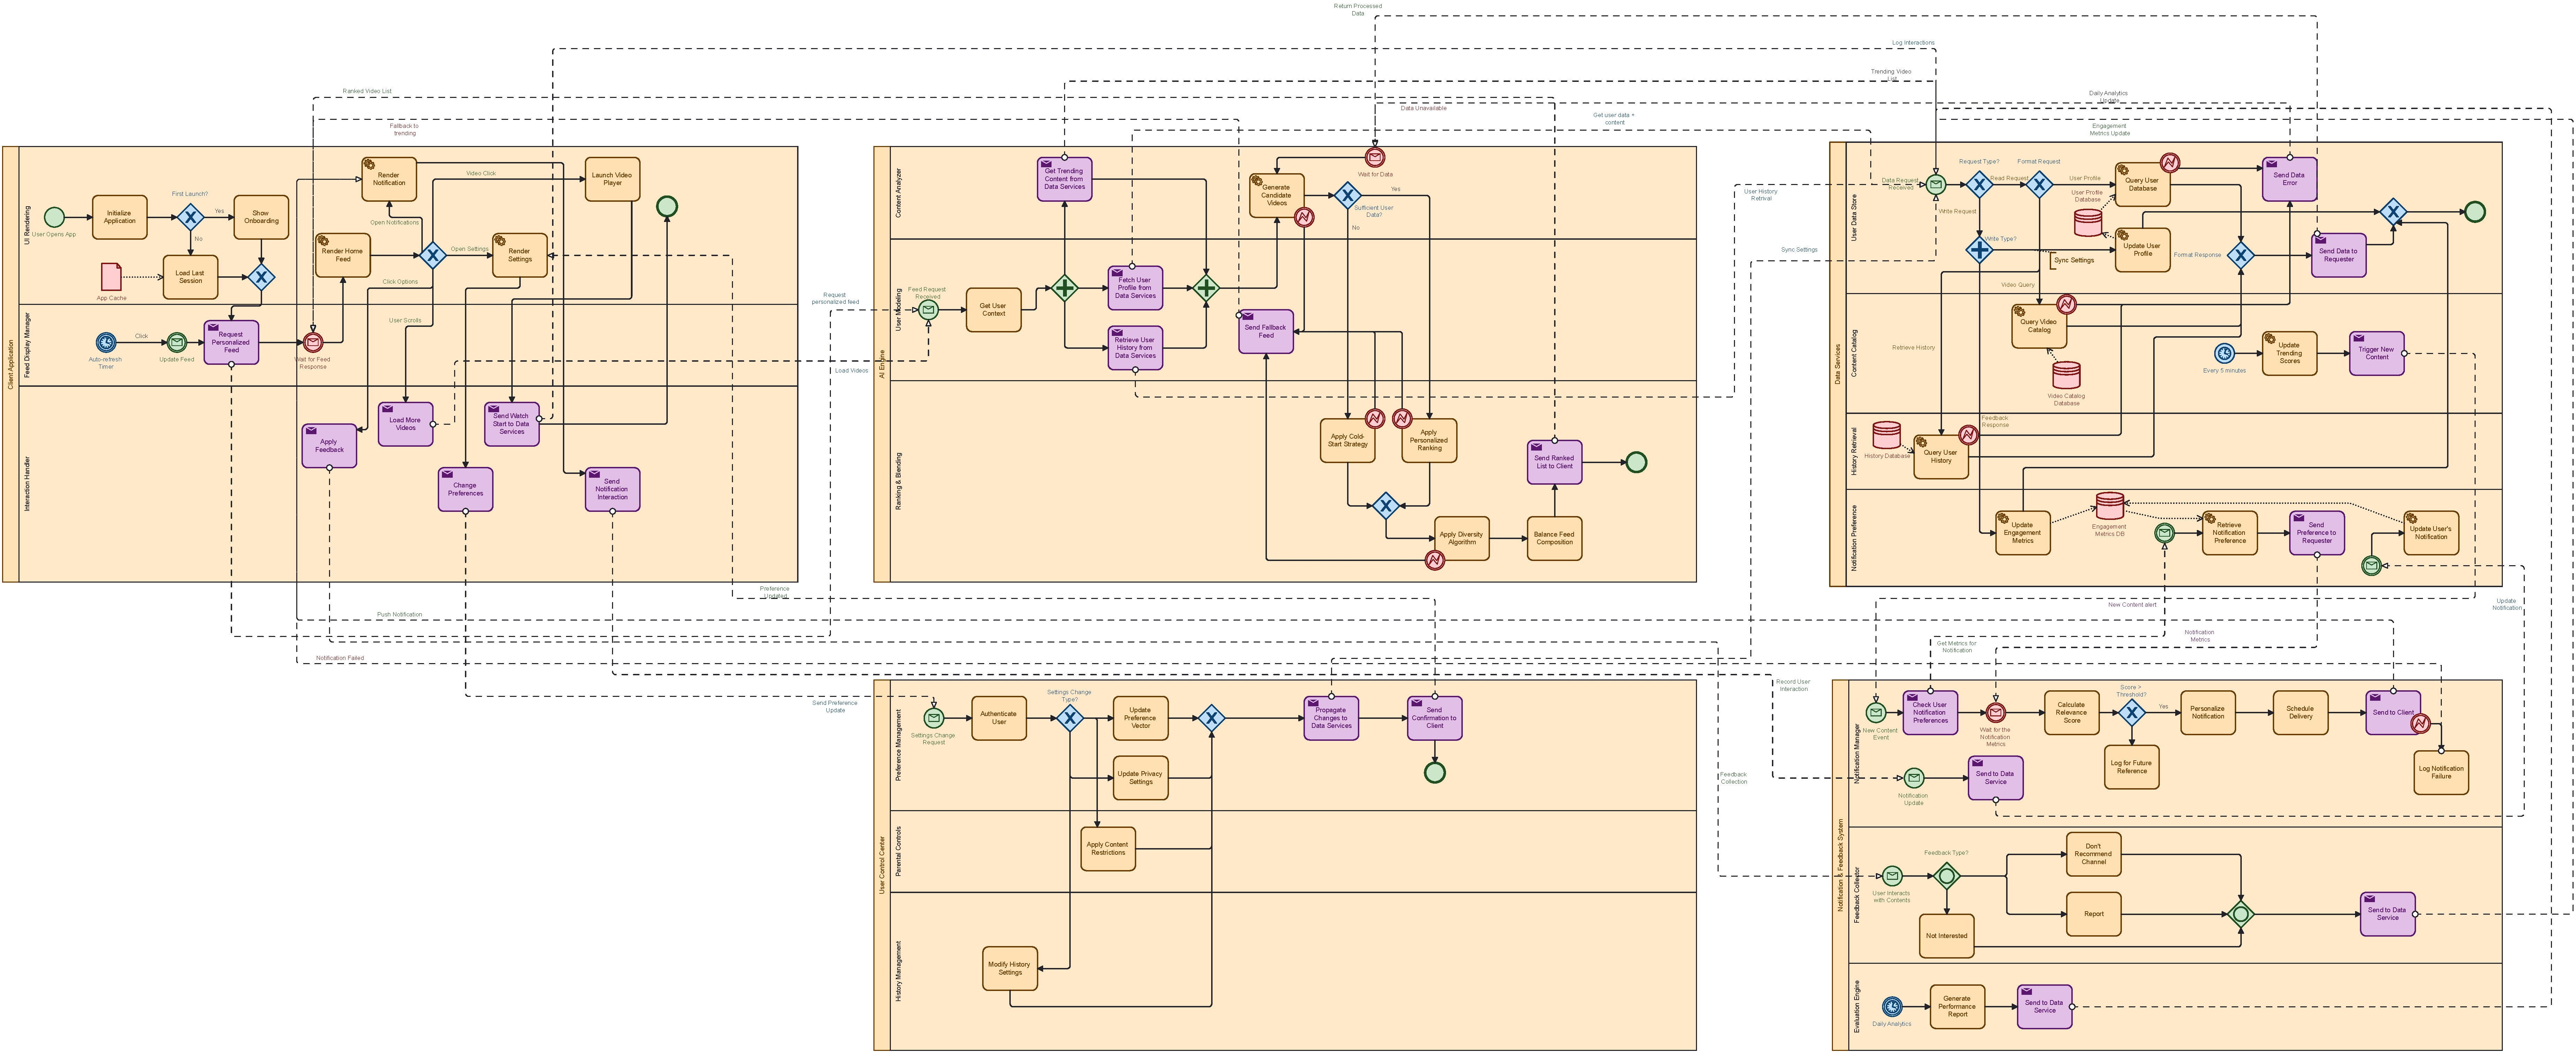
\includegraphics[width=\textheight]{Turjo/turjo_bpmn-v9.pdf}
    \caption{Updated BPMN Diagram of the System Workflow.}
    \label{fig:bpmn}
\end{sidewaysfigure}


% prob bad idea

% \begin{landscape}
%     \begin{figure}[htbp]
%         \centering
%         \includegraphics[width=\linewidth]{Turjo/turjo_bpmn-v10.pdf}
%         \caption{Updated BPMN Diagram of the System Workflow.}
%         \label{fig:bpmn}
%     \end{figure}
% \end{landscape}

% --- CHAPTER 3: USE CASE DIAGRAM ---
\chapter{Use Case Diagram}
\textbf{Presented by: Abhishek Roy (2105033)} \\

\section*{Feedback Implementation}
Based on the feedback received during the presentation regarding lack of details, the following updates and expansions were made to the Use Case Diagram:
\begin{itemize}
    \item \textbf{Actor Renaming:} The actor previously named ``New User'' was changed to \textbf{``Guest User''}, and ``Returning User'' was updated to \textbf{``Registered User''} to align with standard professional and database-level authentication terminology.
    \item \textbf{Generate Video Catalog Details:} Added specific backend processes. Videos are now explicitly run through a diversification algorithm and balanced according to the current feed state.
    \item \textbf{Explicit Feedbacks:} Added granular user interaction capabilities, explicitly specifying \textit{Like, Dislike, Comment,} and \textit{Report} actions.
    \item \textbf{Delete User Feature:} Introduced the account deletion flow, ensuring that the process requires reconfirmation and reauthentication before the major action is executed.
\end{itemize}

\vspace{1cm}

\begin{figure}[p]
    \centering
    \resizebox{\textwidth}{!}{%
        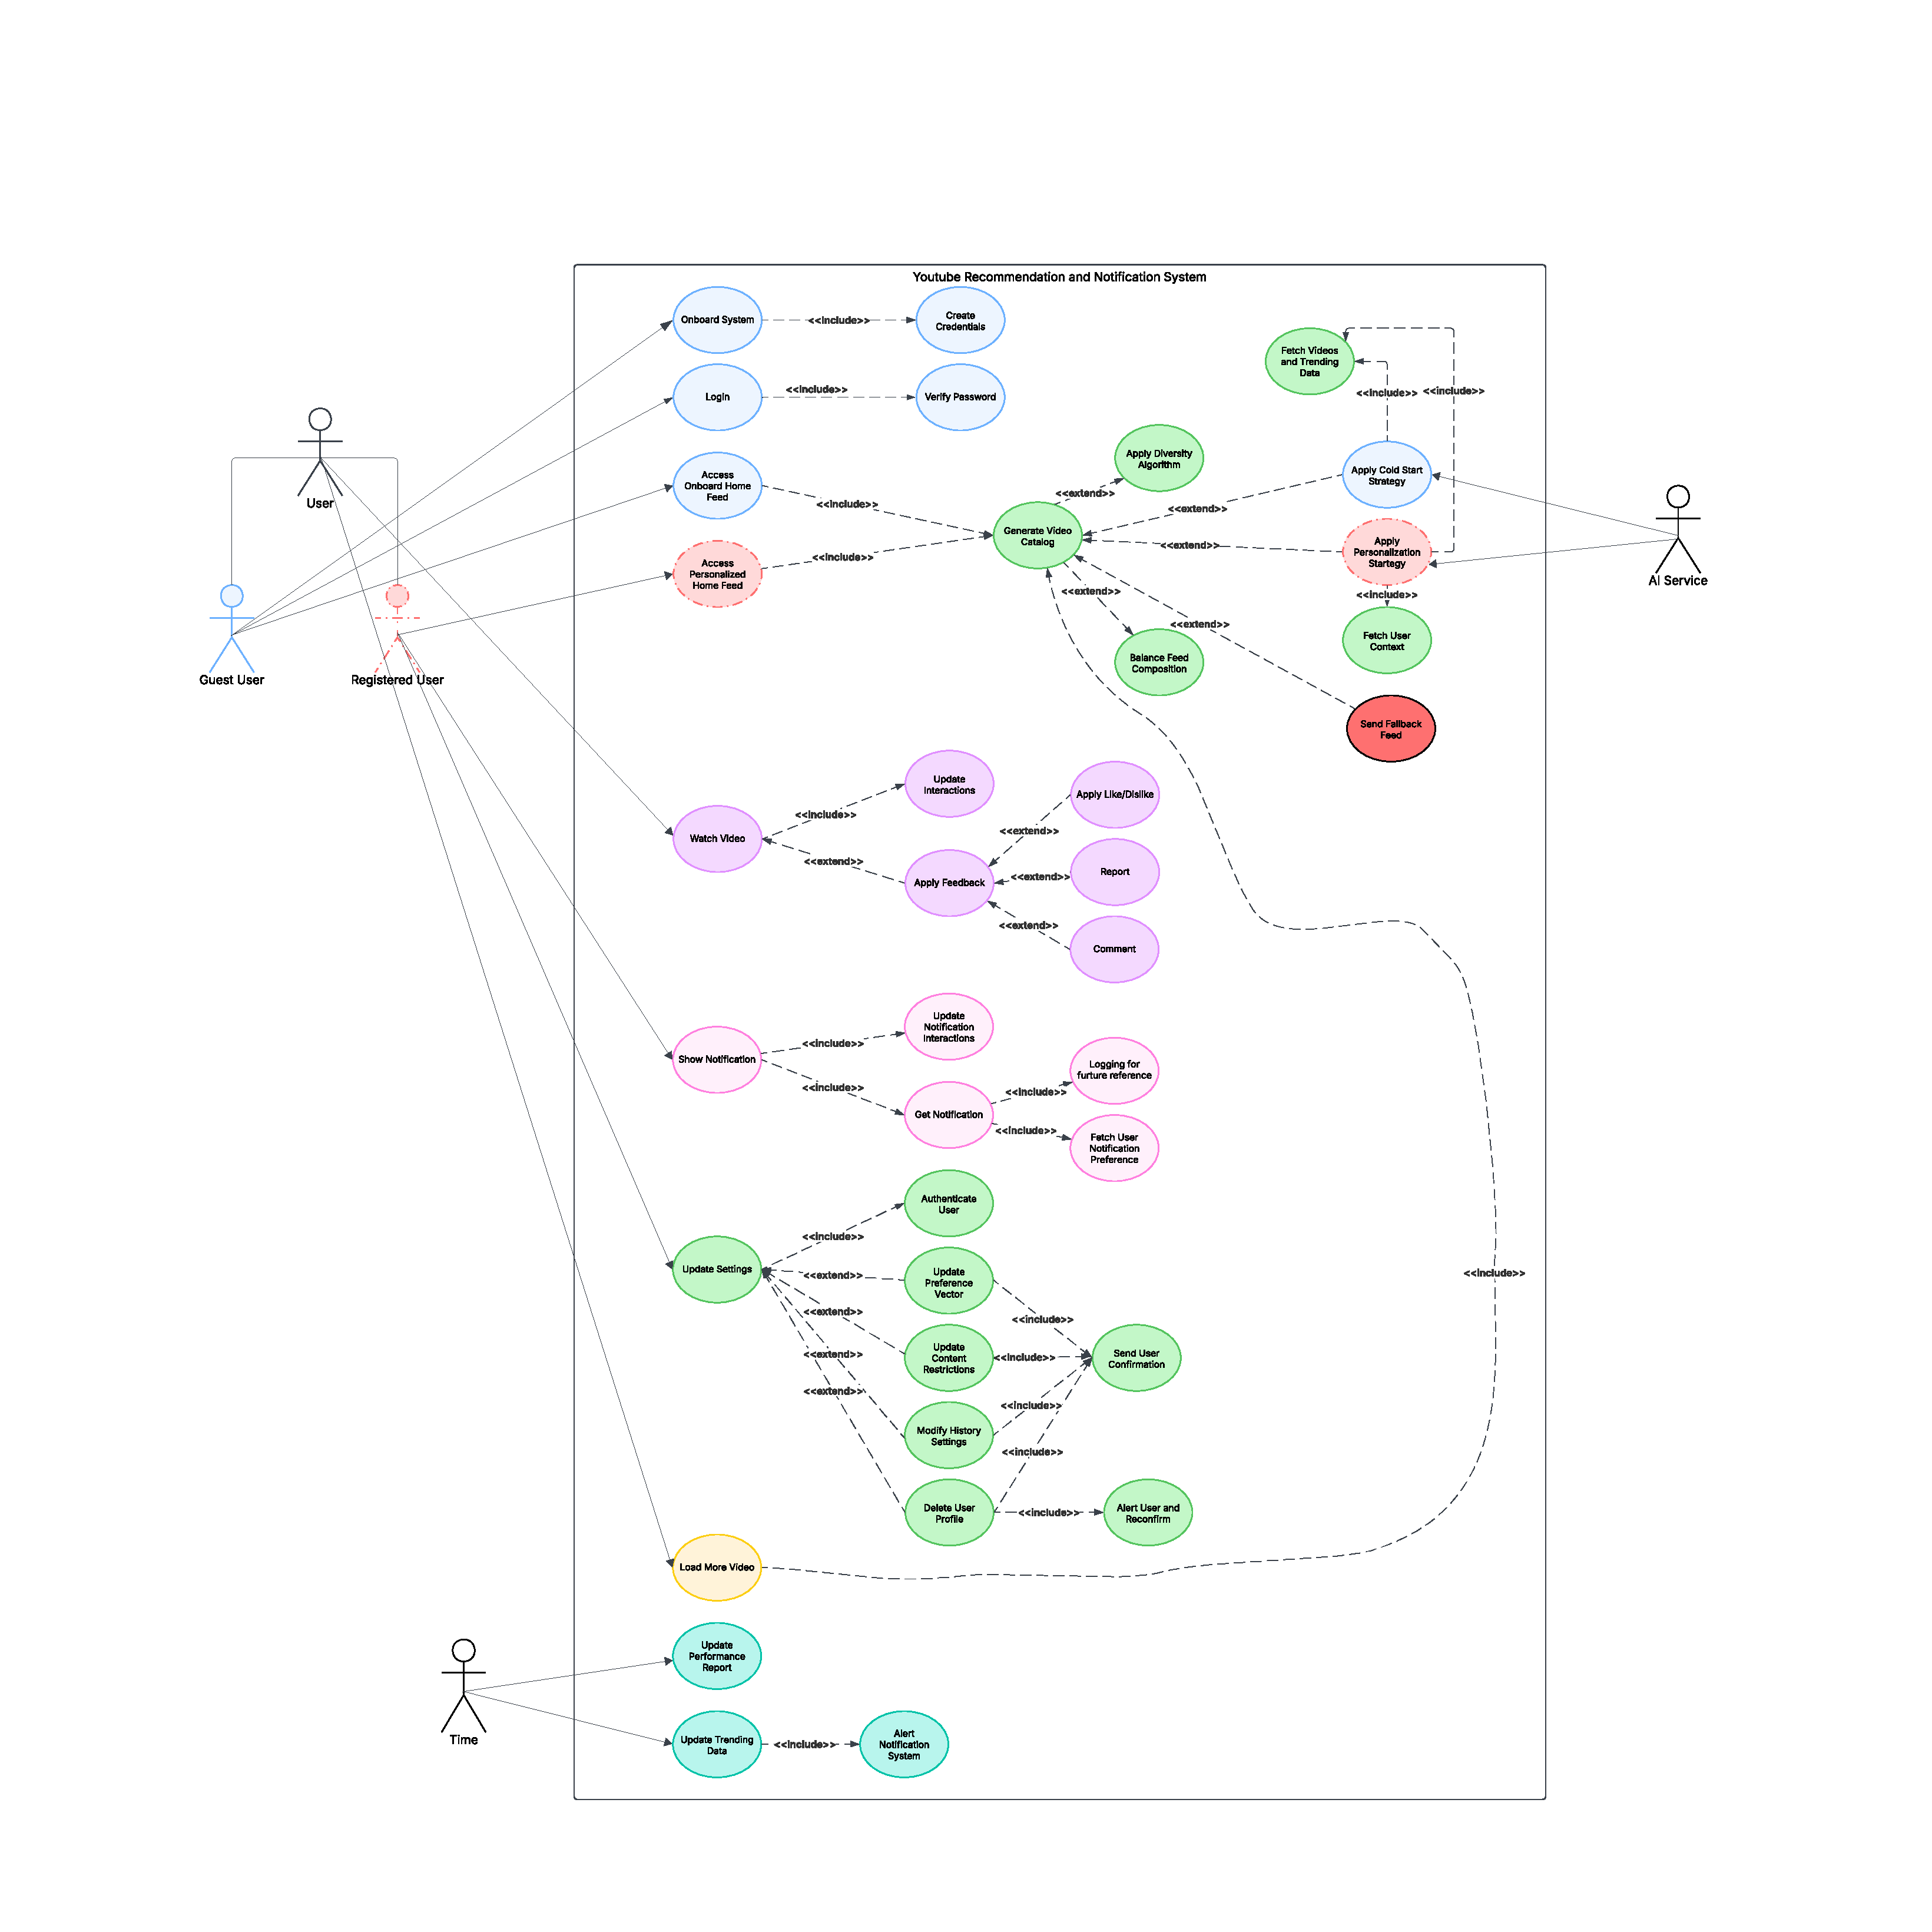
\includegraphics{Abhishek/usecase_v4.pdf}
    }
    \caption{Updated Use Case Diagram. }
    \label{fig:usecase}
\end{figure}

% --- CHAPTER 4: CLASS DIAGRAM ---
\chapter{Class Diagram}
\textbf{Presented by: Abhishek Roy (2105033)} \\

\section*{Feedback Implementation}
Modifications were made to the Class Diagram to address presentation feedback and reflect the architectural shifts required by our database implementation. Specifically, the naming convention issue was addressed by updating class names to properly differentiate between \texttt{GuestUser} and \texttt{RegisteredUser}.

\vspace{1cm}

\begin{figure}[p] % force separate page
    \centering
    \resizebox{\textwidth}{!}{%
        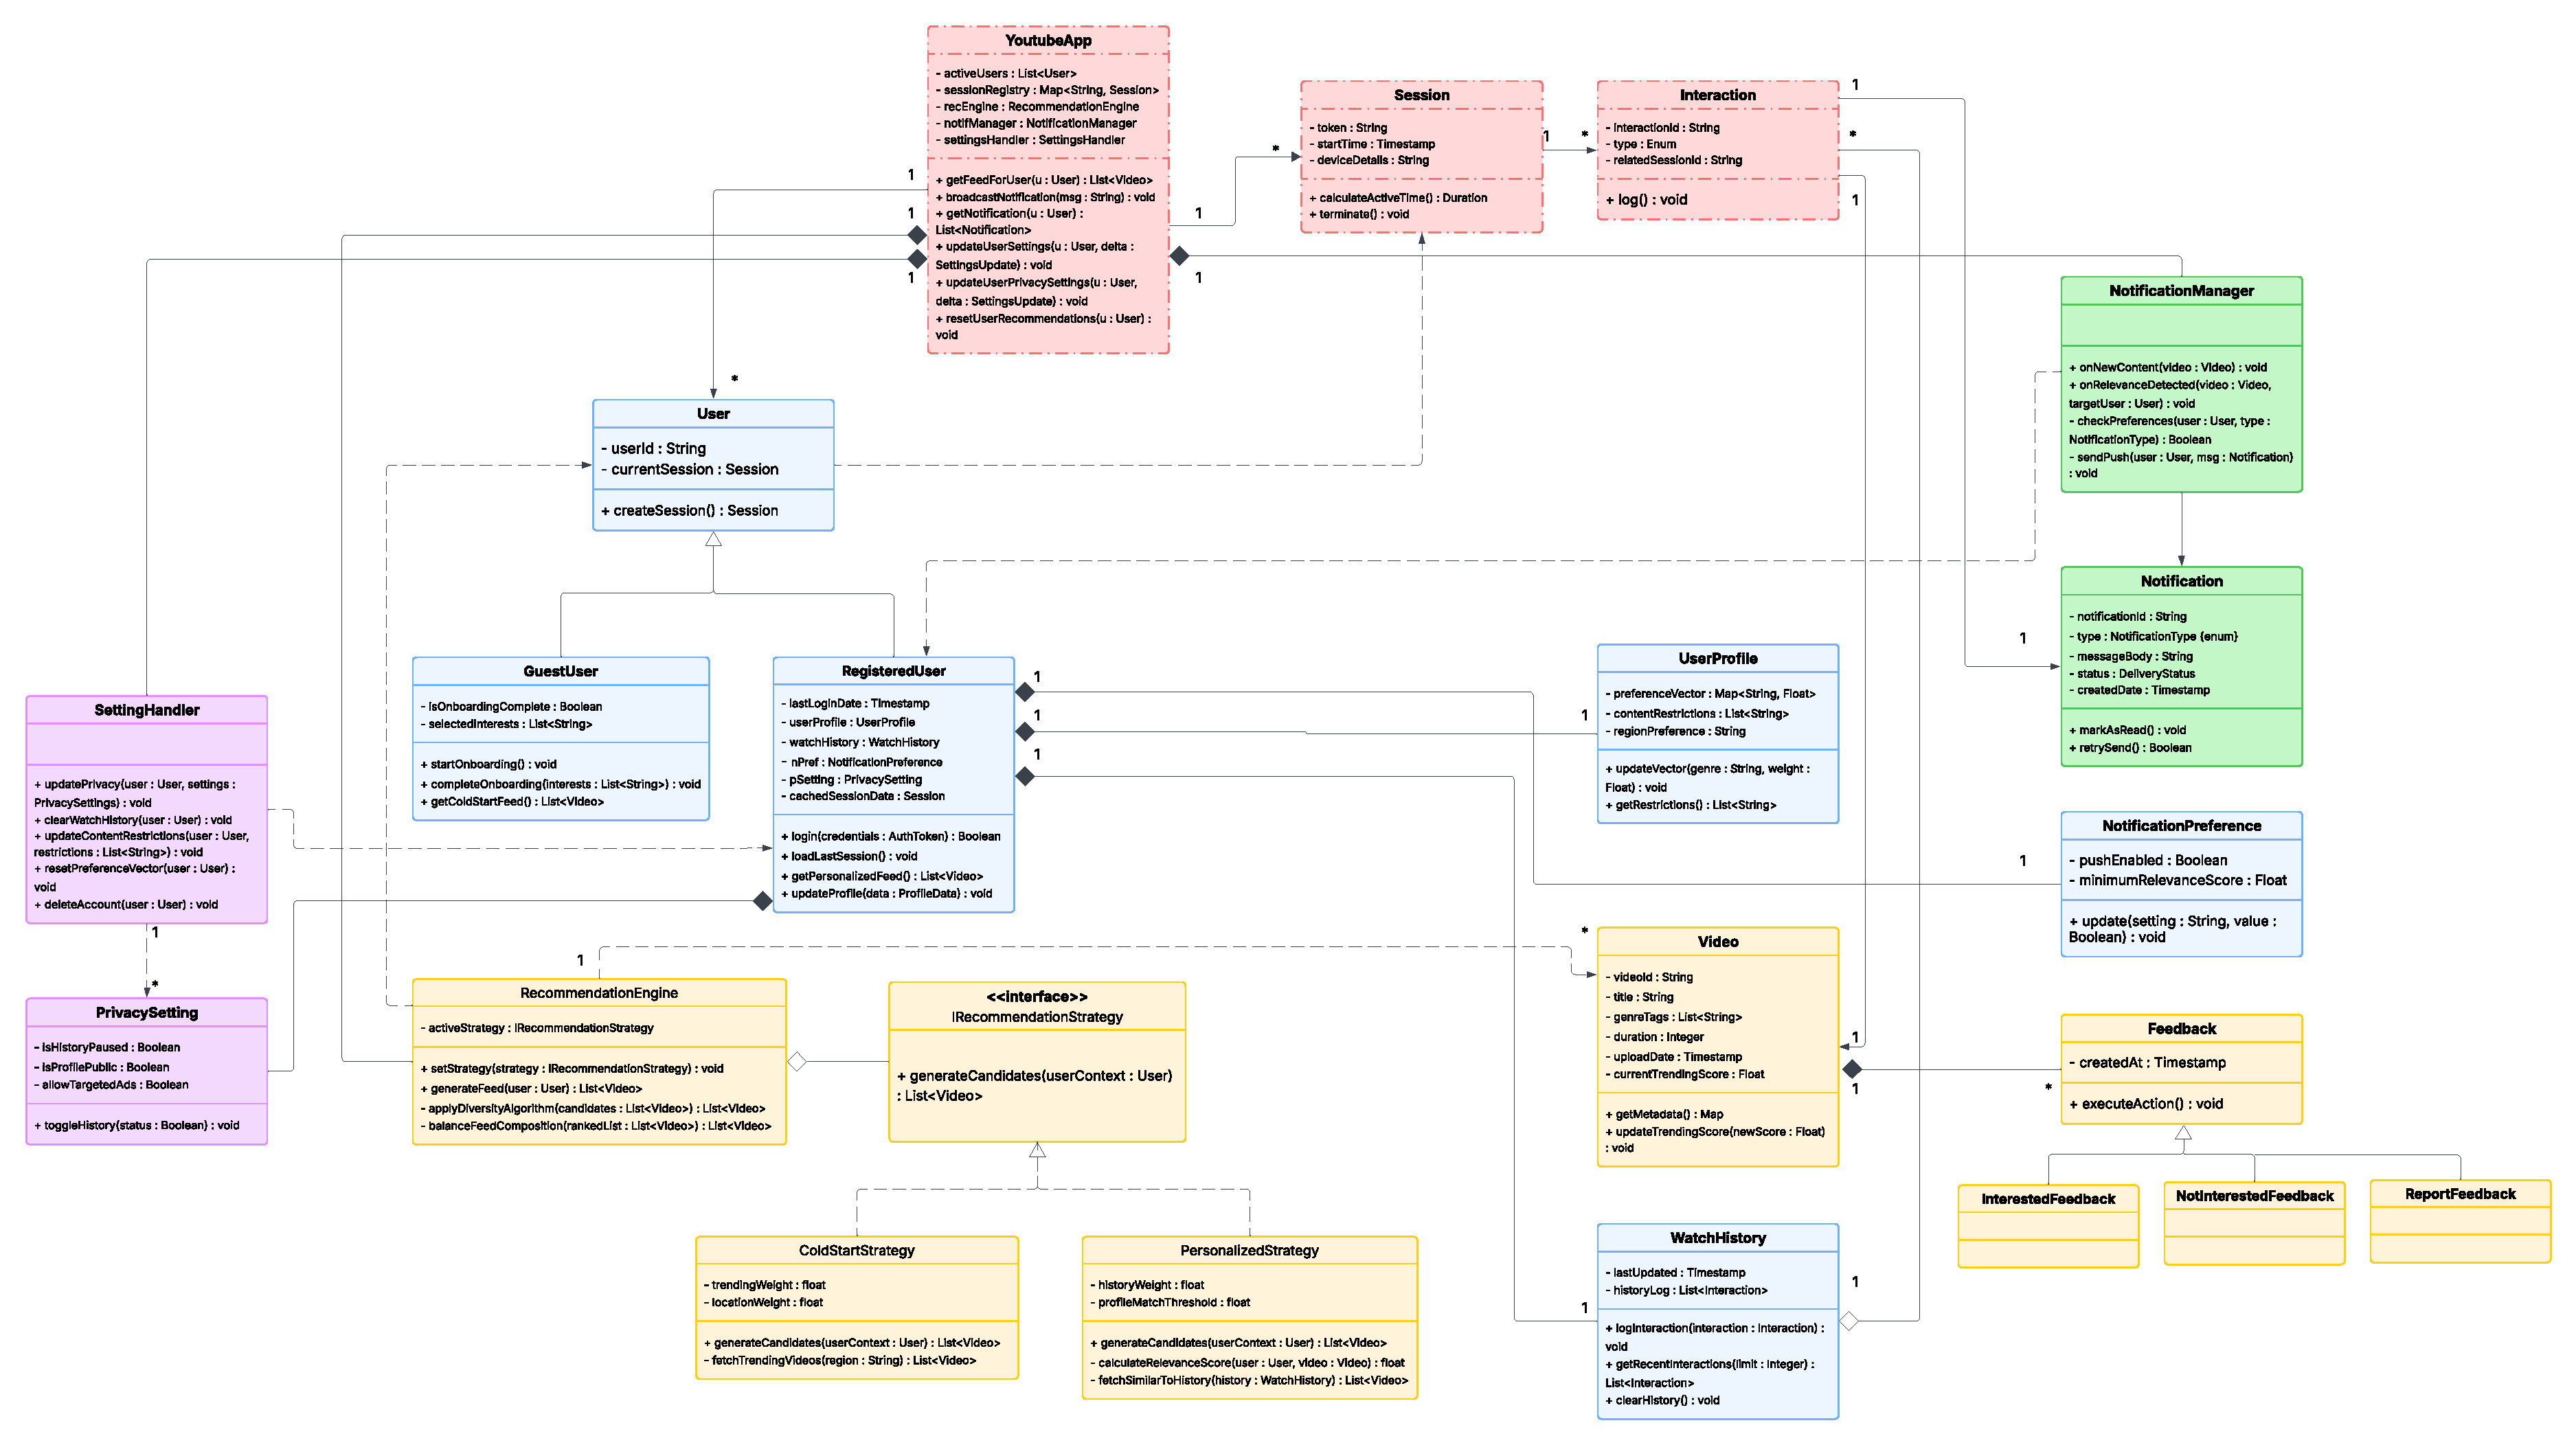
\includegraphics{Abhishek/class_v6.pdf}
    }
    \caption{Updated System Class Diagram.}
    \label{fig:class}
\end{figure}

% --- CHAPTER 5: MOCK UI ---
\chapter{Mock UI}
\textbf{Presented by: Monjur Hossain Khan (2105043)} \\
\section{Key UI Differences with current YouTube}

This redesign introduces several structural changes compared to the current YouTube web application:

\subsection{Tabbed Video Panel}
Current YouTube clutters the screen with separate areas for related videos and live chat. This mockup cleanly consolidates ``Suggestions,'' ``Transcripts,'' and ``Live Chat'' into a single tabbed sidebar, as seen in Figure \ref{fig:mockui_p2}.

\subsection{Subscription Collections}
Instead of an endless, unorganized list of subscribed channels, the sidebar now features ``Collections,'' allowing users to group subscriptions into custom folders like Design or Gaming, as shown in Figure \ref{fig:mockui_p12}.

\subsection{Explicit Feed Customization}
Users gain direct control over their algorithm. A new menu lets users add specific tags to build a custom feed and includes explicit filters to block excluded content, such as ``Shorts,'' referenced in Figure \ref{fig:mockui_p46}.

\subsection{Internal Mutual Sharing}
The Share menu moves beyond external links, adding a native social feature to ``Send to mutual subscribers'' directly within the platform, illustrated in Figure \ref{fig:mockui_p47}[cite: 1626, 1627].

\section*{Feedback Implementation}
Based on presentation feedback, we updated the Mock UI to improve visual accessibility and the overall user experience:

\begin{itemize}
    \item \textbf{Color Contrast \& Theming:} Brightened primary font colors to ensure clear legibility against the dark background.
    \item \textbf{Proportional Sizing \& Legibility:} Increased font sizes for titles to better balance with video thumbnails and improve readability.
\end{itemize}

\vspace{1cm}
% --- PAGE 1 ---
\begin{figure}[htbp]
  \centering
    \includegraphics[width=0.9\textwidth, page=1]{Shovon/YouTube_Mock_UI (Fix).pdf}
    \vspace{0.3cm}\\
    This mockup illustrates the redesigned Homefeed, featuring a cleaner sidebar and a grid of personalized video recommendations.
    \caption{Mock UI - Homefeed Layout}
    \label{fig:mockui_p1}
\end{figure}

% --- PAGE 2 ---
\begin{figure}[htbp]
  \centering
    \includegraphics[width=0.9\textwidth, page=2]{Shovon/YouTube_Mock_UI (Fix).pdf}
    \vspace{0.3cm}\\
    The video playback interface, showing the primary video player, title, channel information, and action buttons.
    \caption{Mock UI - Video Playback Interface}
    \label{fig:mockui_p2}
\end{figure}

% --- PAGE 3 ---
\begin{figure}[htbp]
  \centering
    \includegraphics[width=0.9\textwidth, page=3]{Shovon/YouTube_Mock_UI (Fix).pdf}
    \vspace{0.3cm}\\
    A continued view of the video playback screen, highlighting the collapsible sidebar and related video suggestions.
    \caption{Mock UI - Video Player and Sidebar}
    \label{fig:mockui_p3}
\end{figure}

% --- PAGE 4 ---
\begin{figure}[htbp]
  \centering
    \includegraphics[width=0.9\textwidth, page=4]{Shovon/YouTube_Mock_UI (Fix).pdf}
    \vspace{0.3cm}\\
    The redesigned comments section, featuring filter chips for Top, Newest, and Timed comments alongside the related videos column.
    \caption{Mock UI - Comments Section}
    \label{fig:mockui_p4}
\end{figure}

% --- PAGE 5 ---
\begin{figure}[htbp]
  \centering
    \includegraphics[width=0.9\textwidth, page=5]{Shovon/YouTube_Mock_UI (Fix).pdf}
    \vspace{0.3cm}\\
    This screen demonstrates the Live Chat integration next to the video description, allowing users to interact in real-time.
    \caption{Mock UI - Live Chat Interface}
    \label{fig:mockui_p5}
\end{figure}

% --- PAGE 6 ---
\begin{figure}[htbp]
  \centering
    \includegraphics[width=0.9\textwidth, page=6]{Shovon/YouTube_Mock_UI (Fix).pdf}
    \vspace{0.3cm}\\
    A blank state container for the video player module, showing the base layout for the video controls timeline.
    \caption{Mock UI - Video Player Container State}
    \label{fig:mockui_p6}
\end{figure}

% --- PAGE 7 ---
\begin{figure}[htbp]
  \centering
    \includegraphics[width=0.9\textwidth, page=7]{Shovon/YouTube_Mock_UI (Fix).pdf}
    \vspace{0.3cm}\\
    An expanded view of the Live Chat panel, displaying user messages, moderation badges, and the chat input field.
    \caption{Mock UI - Expanded Live Chat}
    \label{fig:mockui_p7}
\end{figure}

% --- PAGE 8 ---
\begin{figure}[htbp]
  \centering
    \includegraphics[width=0.9\textwidth, page=8]{Shovon/YouTube_Mock_UI (Fix).pdf}
    \vspace{0.3cm}\\
    The "Up Next" and suggested videos column, designed to keep users engaged with algorithmically relevant content.
    \caption{Mock UI - Suggested Videos Column}
    \label{fig:mockui_p8}
\end{figure}

% --- PAGE 9 ---
\begin{figure}[htbp]
  \centering
    \includegraphics[width=0.9\textwidth, page=9]{Shovon/YouTube_Mock_UI (Fix).pdf}
    \vspace{0.3cm}\\
    The trending and category discovery page, featuring larger thumbnails and dedicated sections for Music, Gaming, and Movies.
    \caption{Mock UI - Explore and Trending Feed}
    \label{fig:mockui_p9}
\end{figure}

% --- PAGE 10 ---
\begin{figure}[htbp]
  \centering
    \includegraphics[width=0.9\textwidth, page=10]{Shovon/YouTube_Mock_UI (Fix).pdf}
    \vspace{0.3cm}\\
    The subscriptions feed organized by a timeline view, allowing users to easily catch up on videos from the past 24 hours.
    \caption{Mock UI - Subscriptions Timeline}
    \label{fig:mockui_p10}
\end{figure}

% --- PAGE 11 ---
\begin{figure}[htbp]
  \centering
    \includegraphics[width=0.9\textwidth, page=11]{Shovon/YouTube_Mock_UI (Fix).pdf}
    \vspace{0.3cm}\\
    The subscriptions tab sorted by channel layout, showing recent uploads grouped by the specific content creator.
    \caption{Mock UI - Subscriptions by Channel}
    \label{fig:mockui_p11}
\end{figure}

% --- PAGE 12 ---
\begin{figure}[htbp]
  \centering
    \includegraphics[width=0.9\textwidth, page=12]{Shovon/YouTube_Mock_UI (Fix).pdf}
    \vspace{0.3cm}\\
    A specialized view of subscribed channels categorized by topic, such as Gaming and Tech, for easier navigation.
    \caption{Mock UI - Categorized Subscriptions}
    \label{fig:mockui_p12}
\end{figure}

% --- PAGE 13 ---
\begin{figure}[htbp]
  \centering
    \includegraphics[width=0.9\textwidth, page=13]{Shovon/YouTube_Mock_UI (Fix).pdf}
    \vspace{0.3cm}\\
    A curated Gaming collection feed showing algorithmically recommended gaming trailers, news, and gameplay videos.
    \caption{Mock UI - Gaming Collection Feed}
    \label{fig:mockui_p13}
\end{figure}

% --- PAGE 14 ---
\begin{figure}[htbp]
  \centering
    \includegraphics[width=0.9\textwidth, page=14]{Shovon/YouTube_Mock_UI (Fix).pdf}
    \vspace{0.3cm}\\
    The user's watch history screen, featuring a search bar specifically for finding previously viewed content.
    \caption{Mock UI - Watch History}
    \label{fig:mockui_p14}
\end{figure}

% --- PAGE 15 ---
\begin{figure}[htbp]
  \centering
    \includegraphics[width=0.9\textwidth, page=15]{Shovon/YouTube_Mock_UI (Fix).pdf}
    \vspace{0.3cm}\\
    An "In Case You Missed" recommendation block, designed to resurface high-value content from a user's favorite creators.
    \caption{Mock UI - Missed Content Recommendations}
    \label{fig:mockui_p15}
\end{figure}

% --- PAGE 16 ---
\begin{figure}[htbp]
  \centering
    \includegraphics[width=0.9\textwidth, page=16]{Shovon/YouTube_Mock_UI (Fix).pdf}
    \vspace{0.3cm}\\
    The layout for a Creator's Channel Page, featuring the channel banner, subscriber count, and main video showcase.
    \caption{Mock UI - Creator Channel Page (Home)}
    \label{fig:mockui_p16}
\end{figure}

% --- PAGE 17 ---
\begin{figure}[htbp]
  \centering
    \includegraphics[width=0.9\textwidth, page=17]{Shovon/YouTube_Mock_UI (Fix).pdf}
    \vspace{0.3cm}\\
    The Community Posts tab on a creator's channel, showing text updates and engagement metrics.
    \caption{Mock UI - Channel Community Posts}
    \label{fig:mockui_p17}
\end{figure}

% --- PAGE 18 ---
\begin{figure}[htbp]
  \centering
    \includegraphics[width=0.9\textwidth, page=18]{Shovon/YouTube_Mock_UI (Fix).pdf}
    \vspace{0.3cm}\\
    An expanded view of the Community Posts feed, demonstrating how long-form text and external links are handled.
    \caption{Mock UI - Expanded Community Feed}
    \label{fig:mockui_p18}
\end{figure}

% --- PAGE 19 ---
\begin{figure}[htbp]
  \centering
    \includegraphics[width=0.9\textwidth, page=19]{Shovon/YouTube_Mock_UI (Fix).pdf}
    \vspace{0.3cm}\\
    The "About" section of a creator's channel, displaying the channel description, view statistics, and external social links.
    \caption{Mock UI - Channel About Page}
    \label{fig:mockui_p19}
\end{figure}

% --- PAGE 20 ---
\begin{figure}[htbp]
  \centering
    \includegraphics[width=0.9\textwidth, page=20]{Shovon/YouTube_Mock_UI (Fix).pdf}
    \vspace{0.3cm}\\
    The global search results page, demonstrating how video results, upload dates, and view counts are structured.
    \caption{Mock UI - Search Results Interface}
    \label{fig:mockui_p20}
\end{figure}

% --- PAGE 21 ---
\begin{figure}[htbp]
  \centering
    \includegraphics[width=0.9\textwidth, page=21]{Shovon/YouTube_Mock_UI (Fix).pdf}
    \vspace{0.3cm}\\
    The detailed view of a Playlist, showcasing the total duration, video count, and options to play all or shuffle.
    \caption{Mock UI - Playlist Overview}
    \label{fig:mockui_p21}
\end{figure}

% --- PAGE 22 ---
\begin{figure}[htbp]
  \centering
    \includegraphics[width=0.9\textwidth, page=22]{Shovon/YouTube_Mock_UI (Fix).pdf}
    \vspace{0.3cm}\\
    An expanded view of the playlist contents, showing the ordered list of videos available for consecutive playback.
    \caption{Mock UI - Playlist Contents List}
    \label{fig:mockui_p22}
\end{figure}

% --- PAGE 23 ---
\begin{figure}[htbp]
  \centering
    \includegraphics[width=0.9\textwidth, page=23]{Shovon/YouTube_Mock_UI (Fix).pdf}
    \vspace{0.3cm}\\
    A mixed content feed demonstrating how videos, shorts, and text posts are visually balanced on the screen.
    \caption{Mock UI - Mixed Content Feed}
    \label{fig:mockui_p23}
\end{figure}

% --- PAGE 24 ---
\begin{figure}[htbp]
  \centering
    \includegraphics[width=0.9\textwidth, page=24]{Shovon/YouTube_Mock_UI (Fix).pdf}
    \vspace{0.3cm}\\
    The YouTube Shorts vertical video interface, highlighting the placement of engagement buttons like like, comment, and share.
    \caption{Mock UI - Shorts Player Interface}
    \label{fig:mockui_p24}
\end{figure}

% --- PAGE 25 ---
\begin{figure}[htbp]
  \centering
    \includegraphics[width=0.9\textwidth, page=25]{Shovon/YouTube_Mock_UI (Fix).pdf}
    \vspace{0.3cm}\\
    The expanded left-hand navigation menu layered alongside the "Send Feedback" modal window.
    \caption{Mock UI - Navigation Menu and Feedback}
    \label{fig:mockui_p25}
\end{figure}

% --- PAGE 26 ---
\begin{figure}[htbp]
  \centering
    \includegraphics[width=0.9\textwidth, page=26]{Shovon/YouTube_Mock_UI (Fix).pdf}
    \vspace{0.3cm}\\
    The main Account Settings dashboard where users can manage their channel status, membership, and Google account links.
    \caption{Mock UI - Account Settings Overview}
    \label{fig:mockui_p26}
\end{figure}

% --- PAGE 27 ---
\begin{figure}[htbp]
  \centering
    \includegraphics[width=0.9\textwidth, page=27]{Shovon/YouTube_Mock_UI (Fix).pdf}
    \vspace{0.3cm}\\
    The Notification Settings panel, allowing granular control over push alerts, subscription notifications, and email updates.
    \caption{Mock UI - Notification Settings}
    \label{fig:mockui_p27}
\end{figure}

% --- PAGE 28 ---
\begin{figure}[htbp]
  \centering
    \includegraphics[width=0.9\textwidth, page=28]{Shovon/YouTube_Mock_UI (Fix).pdf}
    \vspace{0.3cm}\\
    Playback and Performance settings, giving users control over video previews, subtitle defaults, and language preferences.
    \caption{Mock UI - Playback Performance Settings}
    \label{fig:mockui_p28}
\end{figure}

% --- PAGE 29 ---
\begin{figure}[htbp]
  \centering
    \includegraphics[width=0.9\textwidth, page=29]{Shovon/YouTube_Mock_UI (Fix).pdf}
    \vspace{0.3cm}\\
    The Privacy Settings dashboard, where users can toggle the visibility of their subscriptions, playlists, and manage ad preferences.
    \caption{Mock UI - Privacy Settings}
    \label{fig:mockui_p29}
\end{figure}

% --- PAGE 30 ---
\begin{figure}[htbp]
  \centering
    \includegraphics[width=0.9\textwidth, page=30]{Shovon/YouTube_Mock_UI (Fix).pdf}
    \vspace{0.3cm}\\
    The Download Settings page, configuring offline viewing quality preferences and storage management options.
    \caption{Mock UI - Download Settings}
    \label{fig:mockui_p30}
\end{figure}

% --- PAGE 31 ---
% \begin{figure}[htbp]
%   \centering
%     \includegraphics[width=0.9\textwidth, page=31]{Shovon/YouTube_Mock_UI (Fix).pdf}
%     \vspace{0.3cm}
%     The empty state placeholder for the "Watch Later" section before a user adds any videos.
%     \caption{Mock UI - Watch Later (Empty State)}
%     \label{fig:mockui_p31}
% \end{figure}

% --- PAGE 32 ---
\begin{figure}[htbp]
  \centering
    \includegraphics[width=0.9\textwidth, page=32]{Shovon/YouTube_Mock_UI (Fix).pdf}
    \vspace{0.3cm}\\
    Various states of the subscription dropdown menu, showing options to filter by posts, videos, live streams, or to unsubscribe.
    \caption{Mock UI - Subscription Dropdown Menus}
    \label{fig:mockui_p32}
\end{figure}

% --- PAGE 33 ---
% \begin{figure}[htbp]
%   \centering
%     \includegraphics[width=0.9\textwidth, page=33]{Shovon/YouTube_Mock_UI (Fix).pdf}
%     \vspace{0.3cm}
%     A collection of individual UI components for notification badges and unread counts.
%     \caption{Mock UI Components - Notification Badges}
%     \label{fig:mockui_p33}
% \end{figure}

% --- PAGE 34 ---
\begin{figure}[htbp]
  \centering
    \includegraphics[width=0.9\textwidth, page=34]{Shovon/YouTube_Mock_UI (Fix).pdf}
    \vspace{0.5cm}\\
    The notifications dropdown panel, displaying recent alerts for channel uploads and shared videos.
    \caption{Mock UI - Notifications Panel}
    \label{fig:mockui_p34}
\end{figure}

% --- PAGES 35, 36, 37, 39 (combined) ---
\begin{figure}[htbp]
  \centering
  \begin{minipage}[t]{0.45\textwidth}
    \centering
    \includegraphics[width=\textwidth, page=35]{Shovon/YouTube_Mock_UI (Fix).pdf}
    \caption{Mock UI - Video Context Menu}
    \label{fig:mockui_p35}
  \end{minipage}\hfill
  \begin{minipage}[t]{0.45\textwidth}
    \centering
    \includegraphics[width=\textwidth, page=36]{Shovon/YouTube_Mock_UI (Fix).pdf}
    \caption{Mock UI - Player Settings Menu}
    \label{fig:mockui_p36}
  \end{minipage}

  \vspace{0.5cm}

  \begin{minipage}[t]{0.45\textwidth}
    \centering
    \includegraphics[width=\textwidth, page=37]{Shovon/YouTube_Mock_UI (Fix).pdf}
    \caption{Mock UI - Advanced Player Controls}
    \label{fig:mockui_p37}
  \end{minipage}\hfill
  \begin{minipage}[t]{0.45\textwidth}
    \centering
    \includegraphics[width=\textwidth, page=39]{Shovon/YouTube_Mock_UI (Fix).pdf}
    \caption{Mock UI - Video Quality Selection}
    \label{fig:mockui_p39}
  \end{minipage}
\end{figure}

% % --- PAGE 40 ---
% \begin{figure}[htbp]
%   \centering
%     \includegraphics[width=0.9\textwidth, page=40]{Shovon/YouTube_Mock_UI (Fix).pdf}
%     \vspace{0.3cm}\\
%     UI component designs for interactive tags and filter chips used in the search and feed generation systems.
%     \caption{Mock UI Components - Tags and Filters}
%     \label{fig:mockui_p40}
% \end{figure}

% % --- PAGE 41 ---
% \begin{figure}[htbp]
%   \centering
%     \includegraphics[width=0.9\textwidth, page=41]{Shovon/YouTube_Mock_UI (Fix).pdf}
%     \vspace{0.3cm}\\
%     A sheet of social media and connected application icons used in the "About" and "Share" sections.
%     \caption{Mock UI Components - Social Icons}
%     \label{fig:mockui_p41}
% \end{figure}

% % --- PAGE 42 ---
% \begin{figure}[htbp]
%   \centering
%     \includegraphics[width=0.9\textwidth, page=42]{Shovon/YouTube_Mock_UI (Fix).pdf}
%     \vspace{0.3cm}\\
%     Various UI interaction elements, including checkboxes, radio buttons, and list item selectors.
%     \caption{Mock UI Components - Checkboxes}
%     \label{fig:mockui_p42}
% \end{figure}

% --- PAGES 43, 45, 46 (combined) ---
\begin{figure}[htbp]
  \centering
  \begin{minipage}[t]{0.45\textwidth}
    \centering
    \includegraphics[width=\textwidth, page=43]{Shovon/YouTube_Mock_UI (Fix).pdf}
    \caption{Mock UI Components - Tab Navigation}
    \label{fig:mockui_p43}
  \end{minipage}\hfill
  \begin{minipage}[t]{0.45\textwidth}
    \centering
    \includegraphics[width=\textwidth, page=45]{Shovon/YouTube_Mock_UI (Fix).pdf}
    \caption{Mock UI Components - Sidebar Tabs}
    \label{fig:mockui_p45}
  \end{minipage}

  \vspace{0.5cm}

  \begin{minipage}[t]{0.65\textwidth}
    \centering
    \includegraphics[width=\textwidth, page=46]{Shovon/YouTube_Mock_UI (Fix).pdf}
    \caption{Mock UI - Personalized Feed Settings}
    \label{fig:mockui_p46}
  \end{minipage}
\end{figure}

% --- PAGE 47 ---
\begin{figure}[htbp]
  \centering
    \includegraphics[width=0.9\textwidth, page=47]{Shovon/YouTube_Mock_UI (Fix).pdf}
    \vspace{0.3cm}\\
    The expanded Share modal, providing quick access to mutual subscribers, messaging apps, and a copyable video link.
    \caption{Mock UI - Share Menu Modal}
    \label{fig:mockui_p47}
\end{figure}


% --- CHAPTER 6: COLLABORATION DIAGRAM ---
\chapter{Collaboration Diagram}
\textbf{Presented by: Shams Hossain Simanto (2105048)} \\

\noindent
Based on the feedback received, the following improvements have been implemented in the revised version of the YouTube Recommendation and Personalization System documentation:

\begin{itemize}
    \item \textbf{Numbering corrections} – Previously, the function sequence numbering contained inconsistencies and formatting errors (repetitive decimal notations). These have been systematically corrected to ensure a clear and logical flow of operations across all sequence diagrams.

    \item \textbf{Enhanced flow representation} – The onboarding, login, and feed generation steps have been re-sequenced and relabeled for better clarity (explicit calls to \texttt{applyDiversityAlgo()} and \texttt{balanceFeedComposition()}).

    \item \textbf{Performance tracking} – The \texttt{updatePerformanceReport()} method, previously absent, has been included to support system monitoring and evaluation.
\end{itemize}

\vspace{1cm}
% \begin{figure}[htbp]
%   \centering
%   \framebox{\parbox{0.8\textwidth}{\centering
%     \vspace{3cm}
%     \textbf{PDF Placeholder} \\
%     \small\textit{Insert Collaboration Diagram PDF Here.}
%     \vspace{3cm}
%   }}
%   \caption{System Collaboration Diagram.}
%   \label{fig:collab}
% \end{figure}

\begin{figure}[htbp]
    \centering
    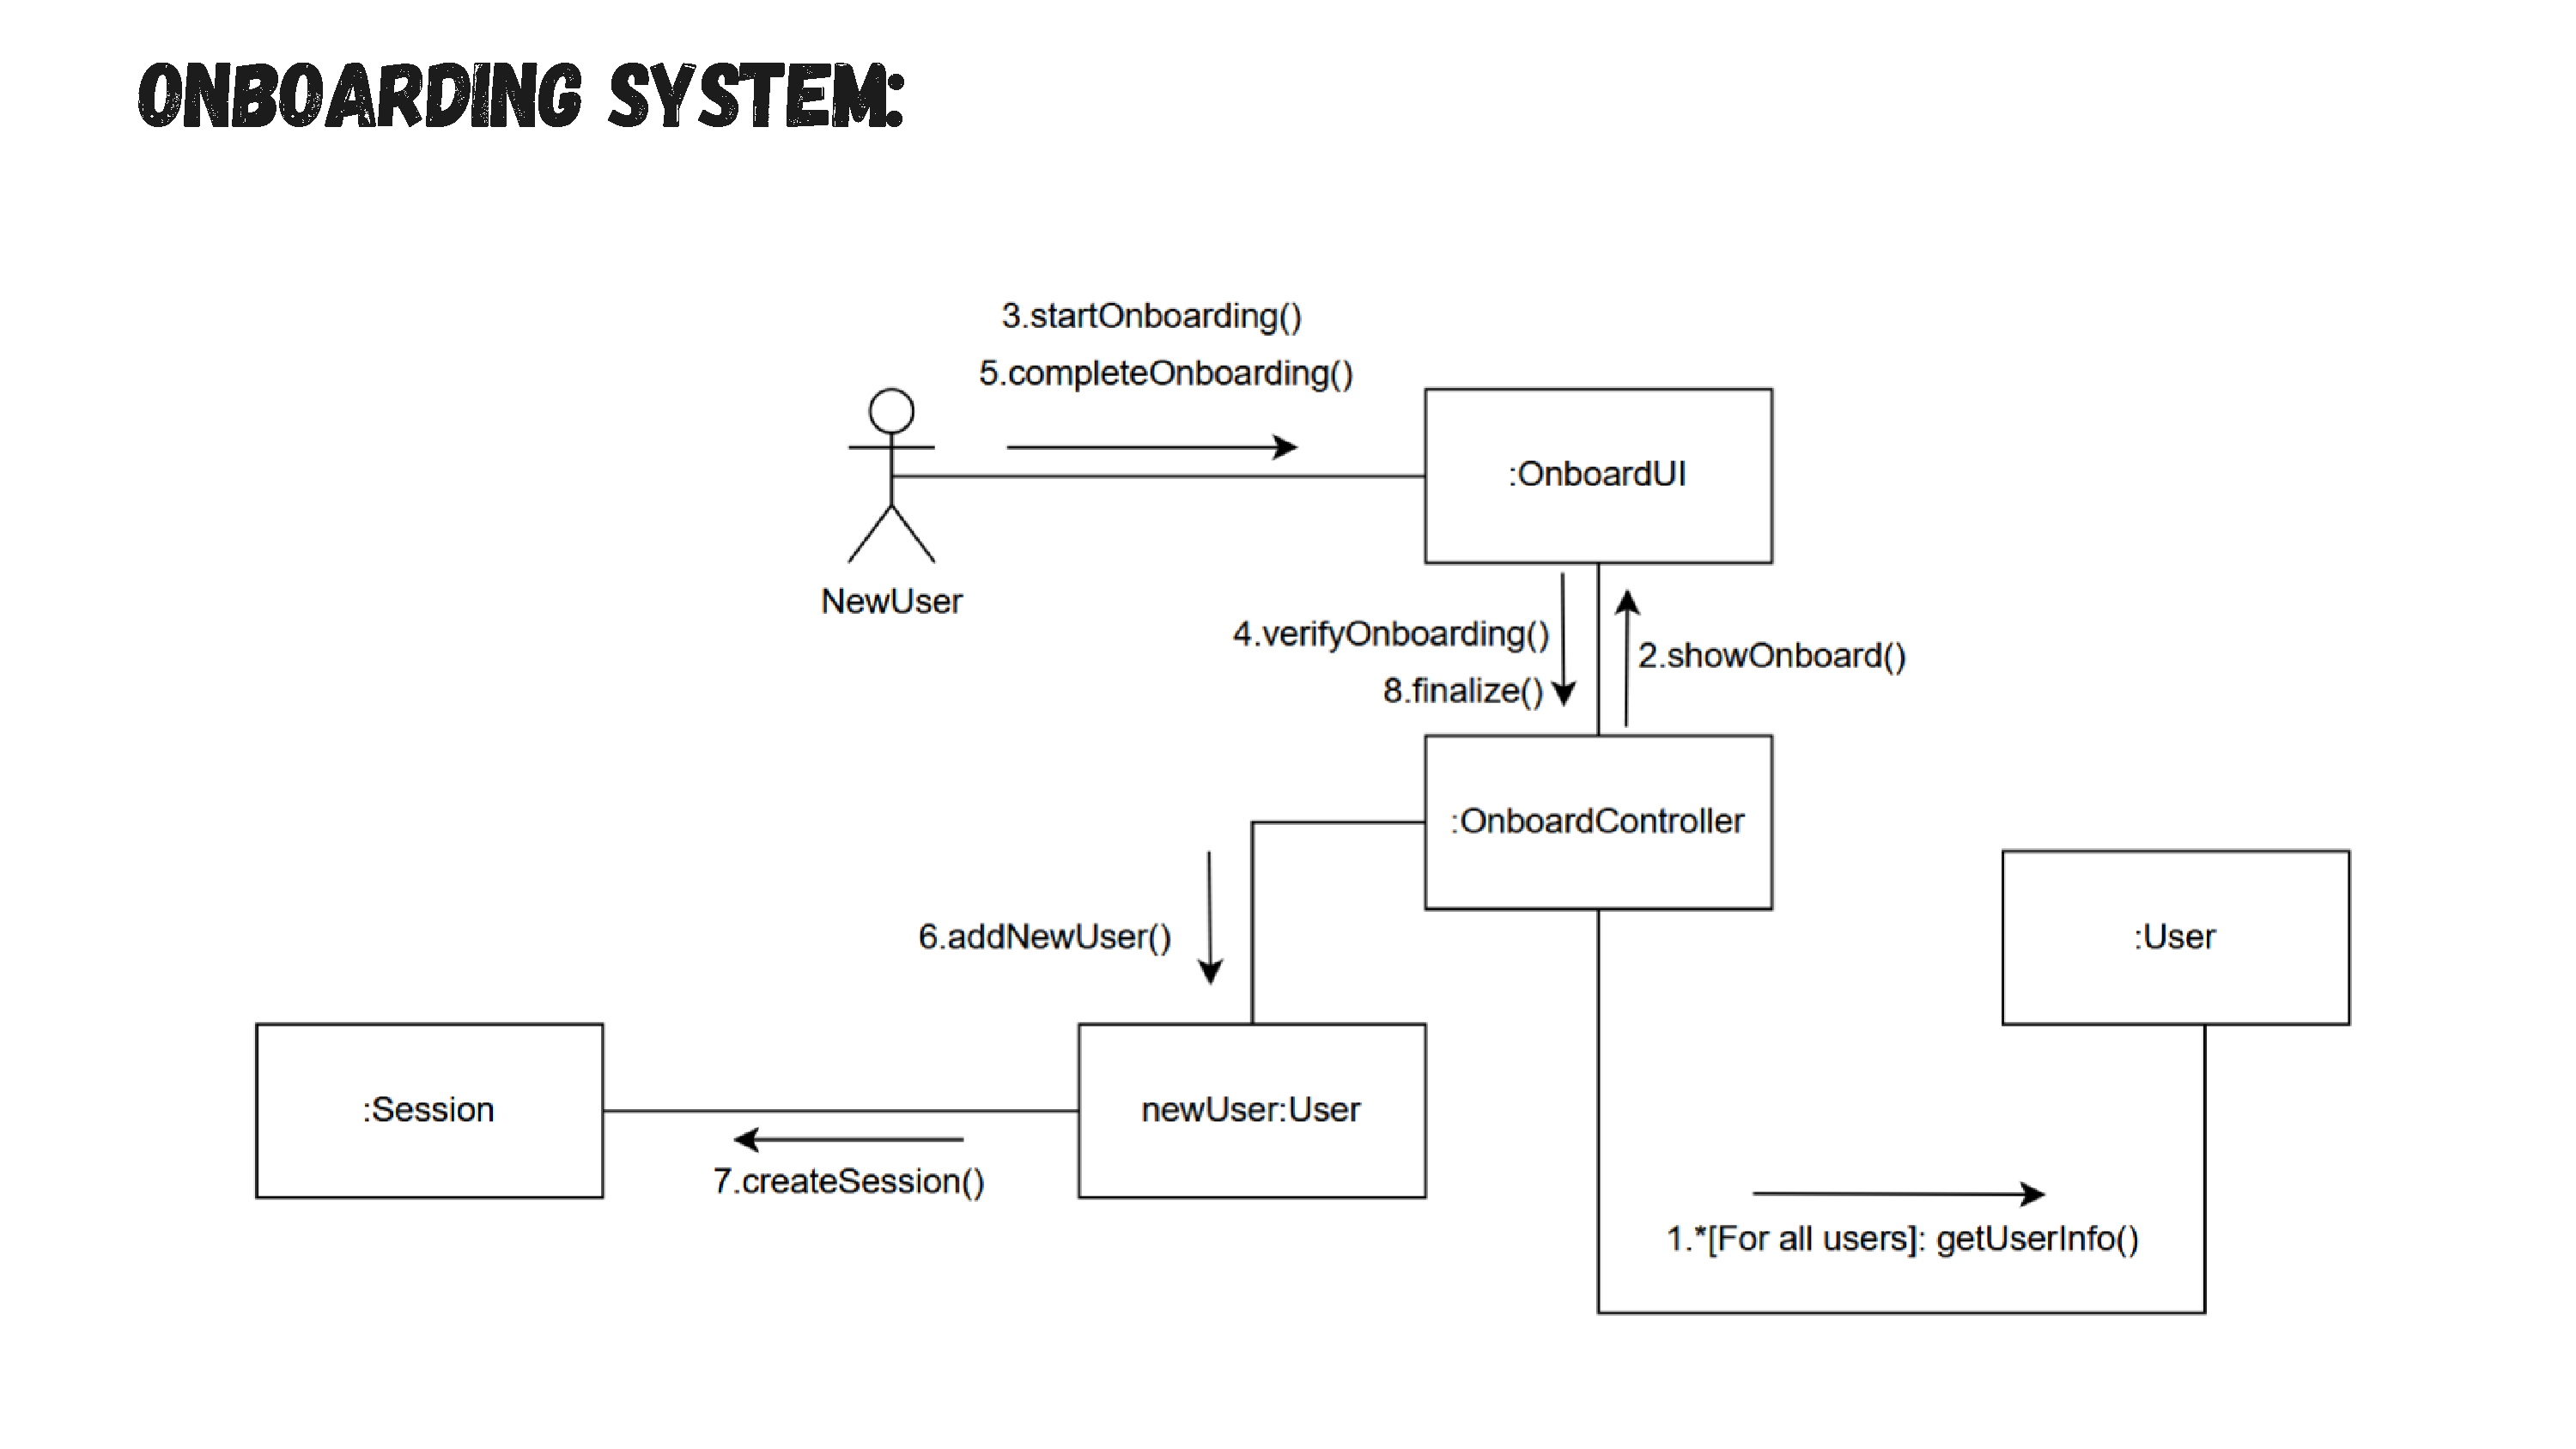
\includegraphics[width=\textwidth, height=0.85\textheight, keepaspectratio]{Simanto/Collab.pdf}
    \caption{Collaboration Diagram For Onboarding System}
\end{figure}

\begin{figure}[htbp]
    \centering
    \includegraphics[width=\textwidth, height=0.85\textheight, keepaspectratio, page=2]{Simanto/Collab.pdf}
    \caption{Collaboration Diagram For Login System}
\end{figure}

\begin{figure}[htbp]
    \centering
    \includegraphics[width=\textwidth, height=0.85\textheight, keepaspectratio, page=3]{Simanto/Collab.pdf}
    \caption{Collaboration Diagram For Homefeed Interaction For New User}
\end{figure}

\begin{figure}[htbp]
    \centering
    \includegraphics[width=\textwidth, height=0.85\textheight, keepaspectratio, page=4]{Simanto/Collab.pdf}
    \caption{Collaboration Diagram For Homefeed Interaction For Returning User}
\end{figure}

\begin{figure}[htbp]
    \centering
    \includegraphics[width=\textwidth, height=0.85\textheight, keepaspectratio, page=5]{Simanto/Collab.pdf}
    \caption{Collaboration Diagram For Video Interaction For User}
\end{figure}

\begin{figure}[htbp]
    \centering
    \includegraphics[width=\textwidth, height=0.85\textheight, keepaspectratio, page=6]{Simanto/Collab.pdf}
    \caption{Sequence Diagram For Notification System}
\end{figure}


\begin{figure}[htbp]
    \centering
    \includegraphics[width=\textwidth, height=0.85\textheight, keepaspectratio, page=7]{Simanto/Collab.pdf}
    \caption{Sequence Diagram For Preference And Personalized Control}
\end{figure}


\begin{figure}[htbp]
    \centering
    \includegraphics[width=\textwidth, height=0.85\textheight, keepaspectratio, page=8]{Simanto/Collab.pdf}
    \caption{Sequence Diagram For Analysis And Tracking}
\end{figure}



% --- CHAPTER 7: SEQUENCE DIAGRAM ---
\chapter{Sequence Diagram}
\textbf{Presented by: Amit Saha (2105049)} \\

\section*{Feedback Implementation}
No updates were needed for the sequence diagrams based on the presentation. Here are the diagrams.

\vspace{1cm}

\begin{figure}[htbp]
    \centering
    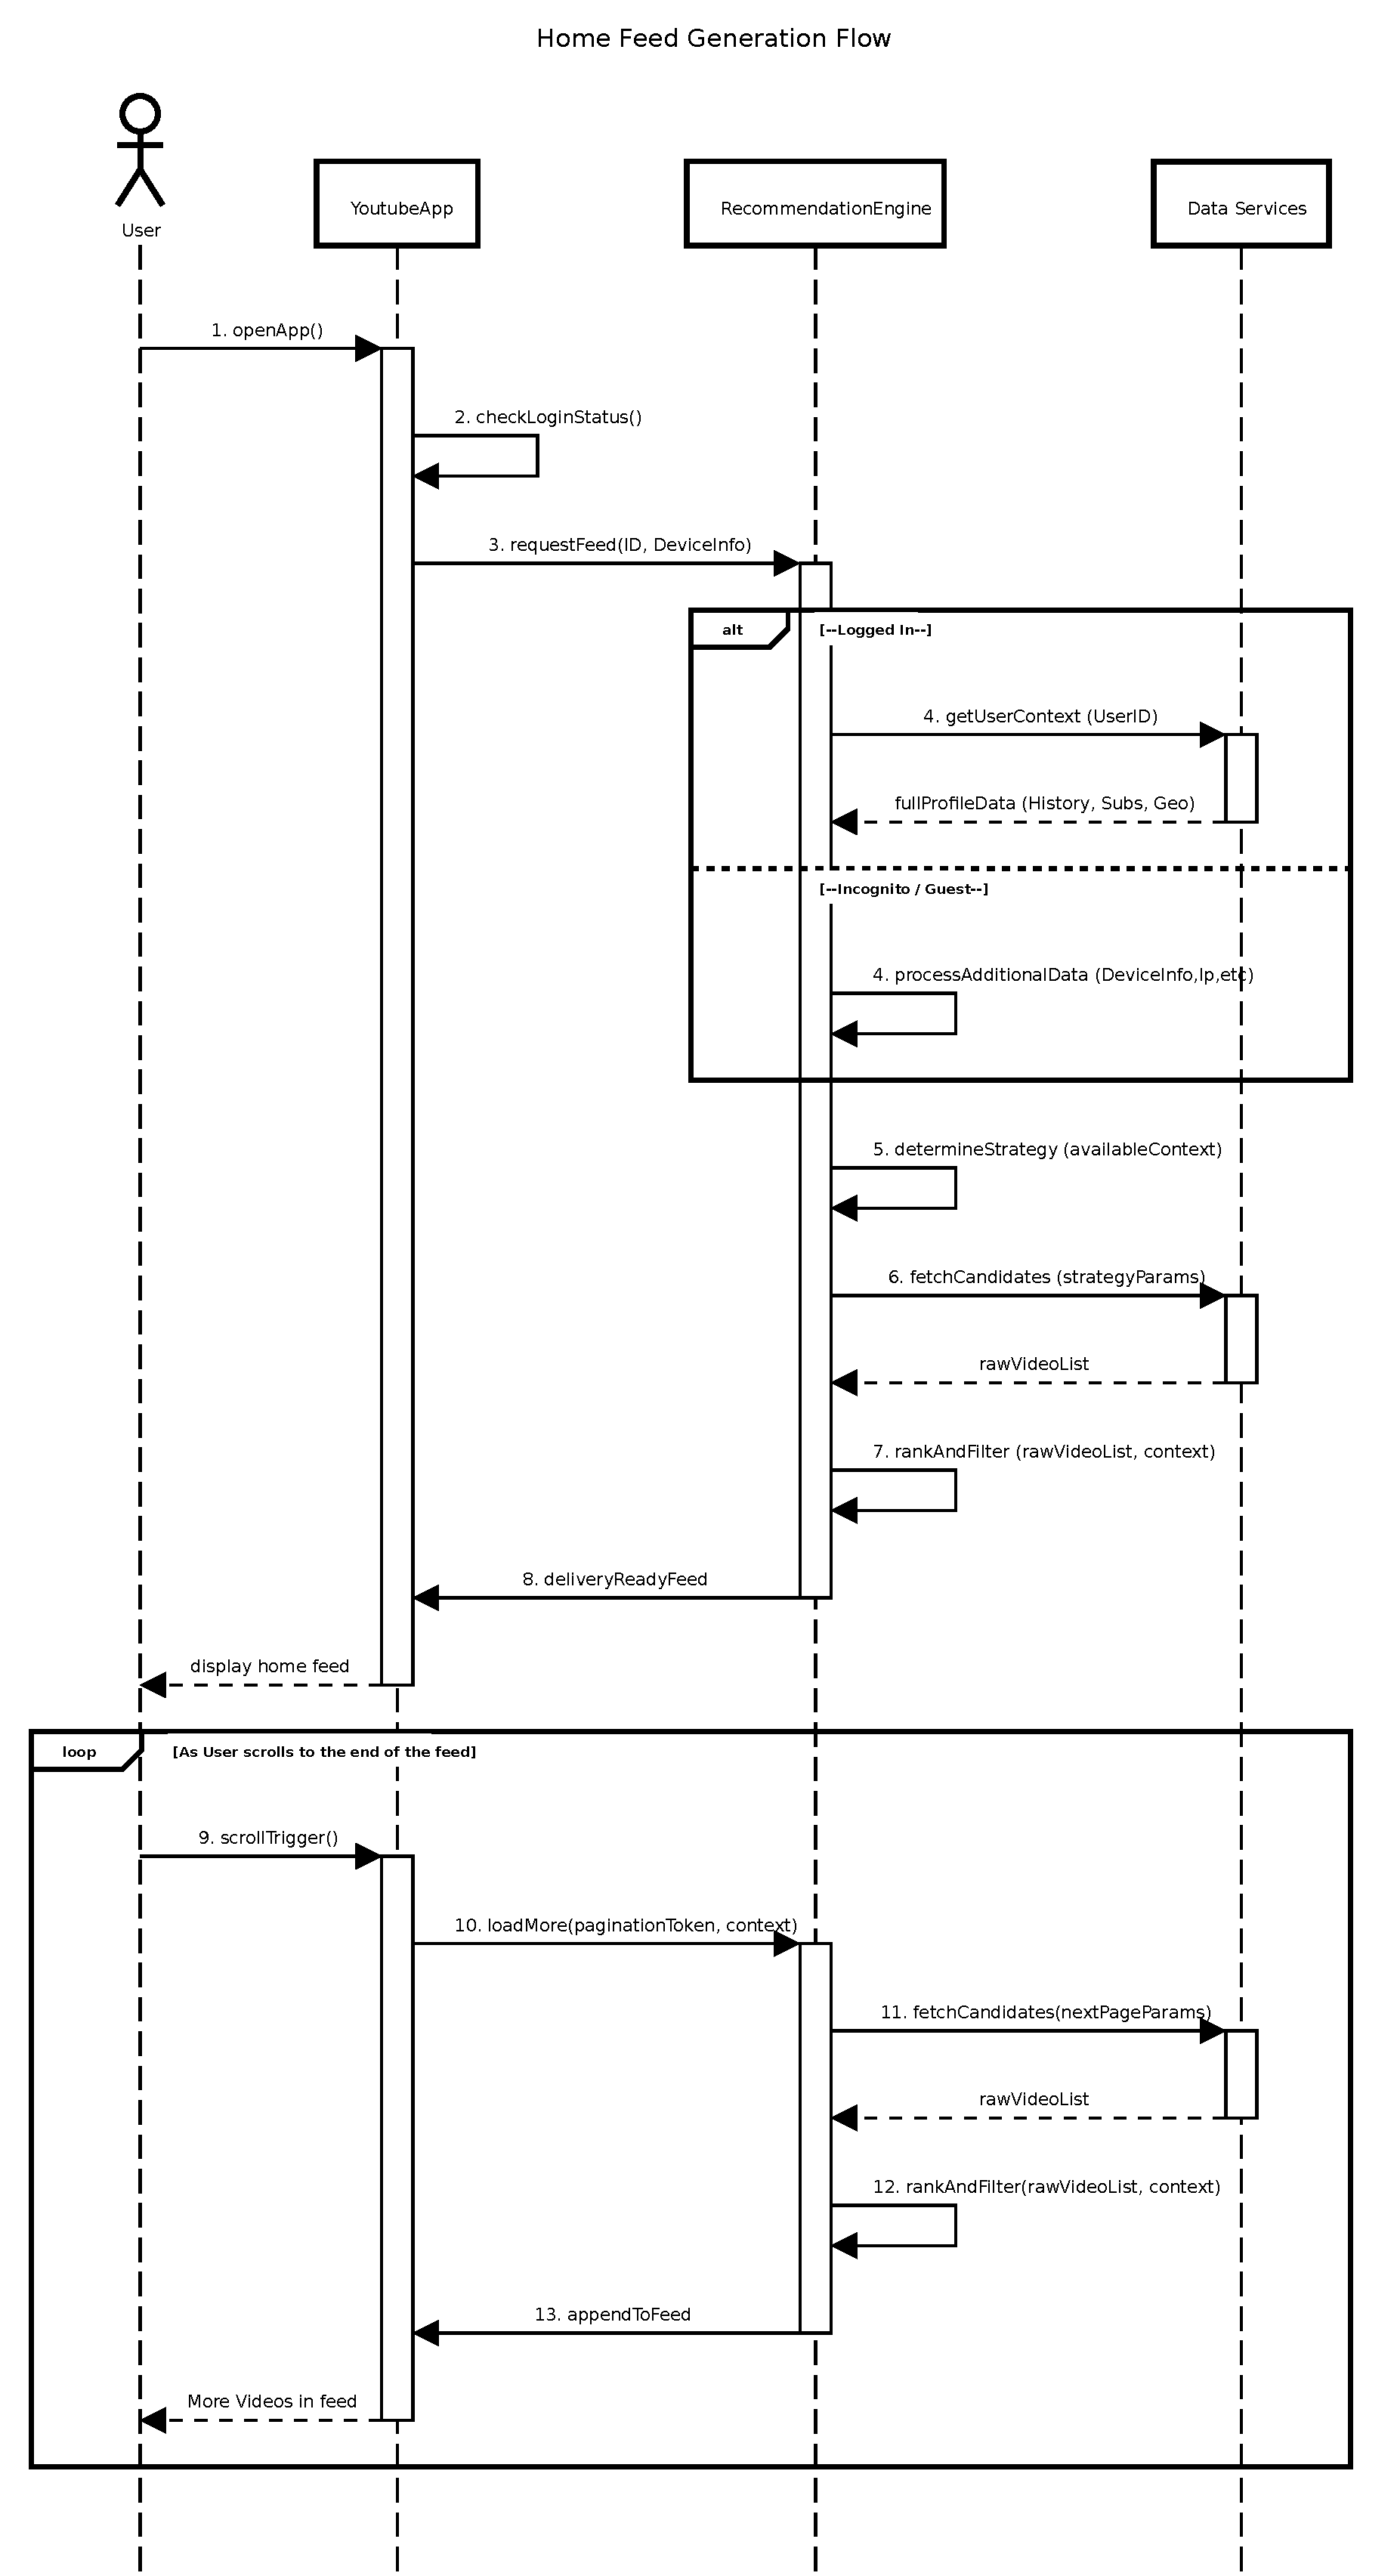
\includegraphics[width=\textwidth, height=0.85\textheight, keepaspectratio]{amit/sequence/homefeed_222.pdf}
    \caption{Sequence Diagram for Homefeed Generation}
\end{figure}

\begin{figure}[htbp]
    \centering
    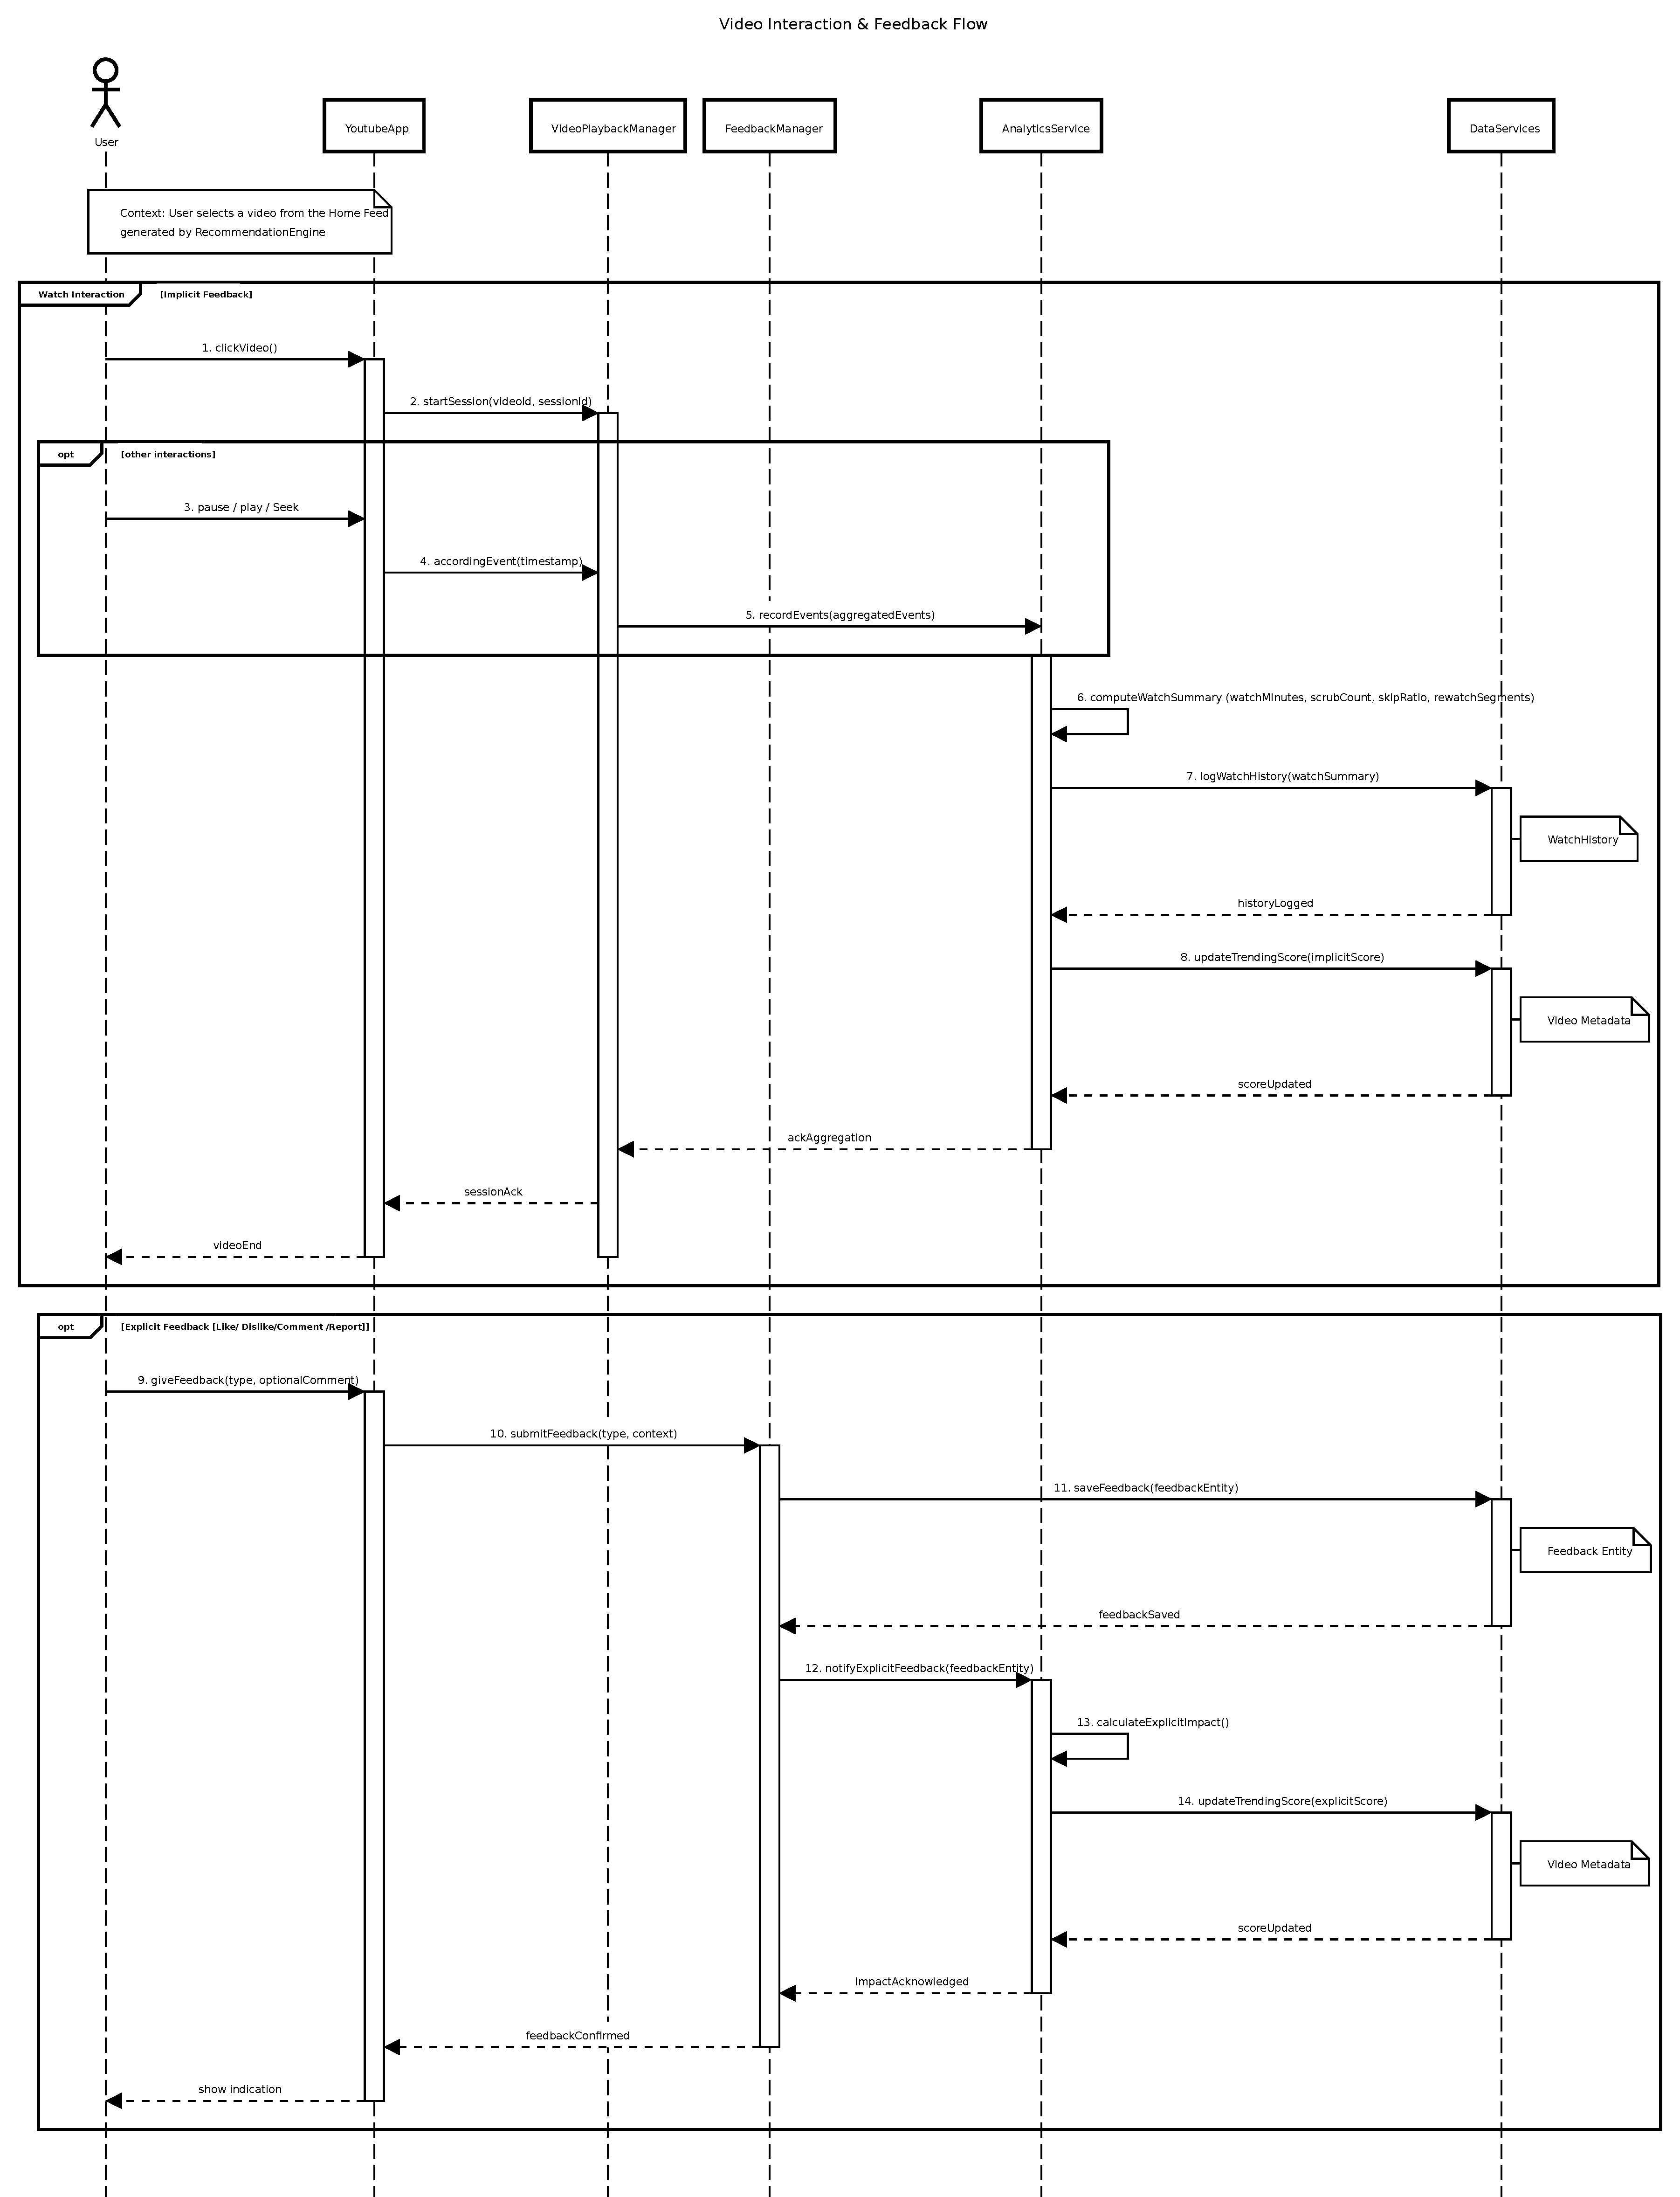
\includegraphics[width=\textwidth, height=0.85\textheight, keepaspectratio]{amit/sequence/videoplay_final.pdf}
    \caption{Sequence Diagram for Video Interaction and Feedback Flow}
\end{figure}

\begin{figure}[htbp]
    \centering
    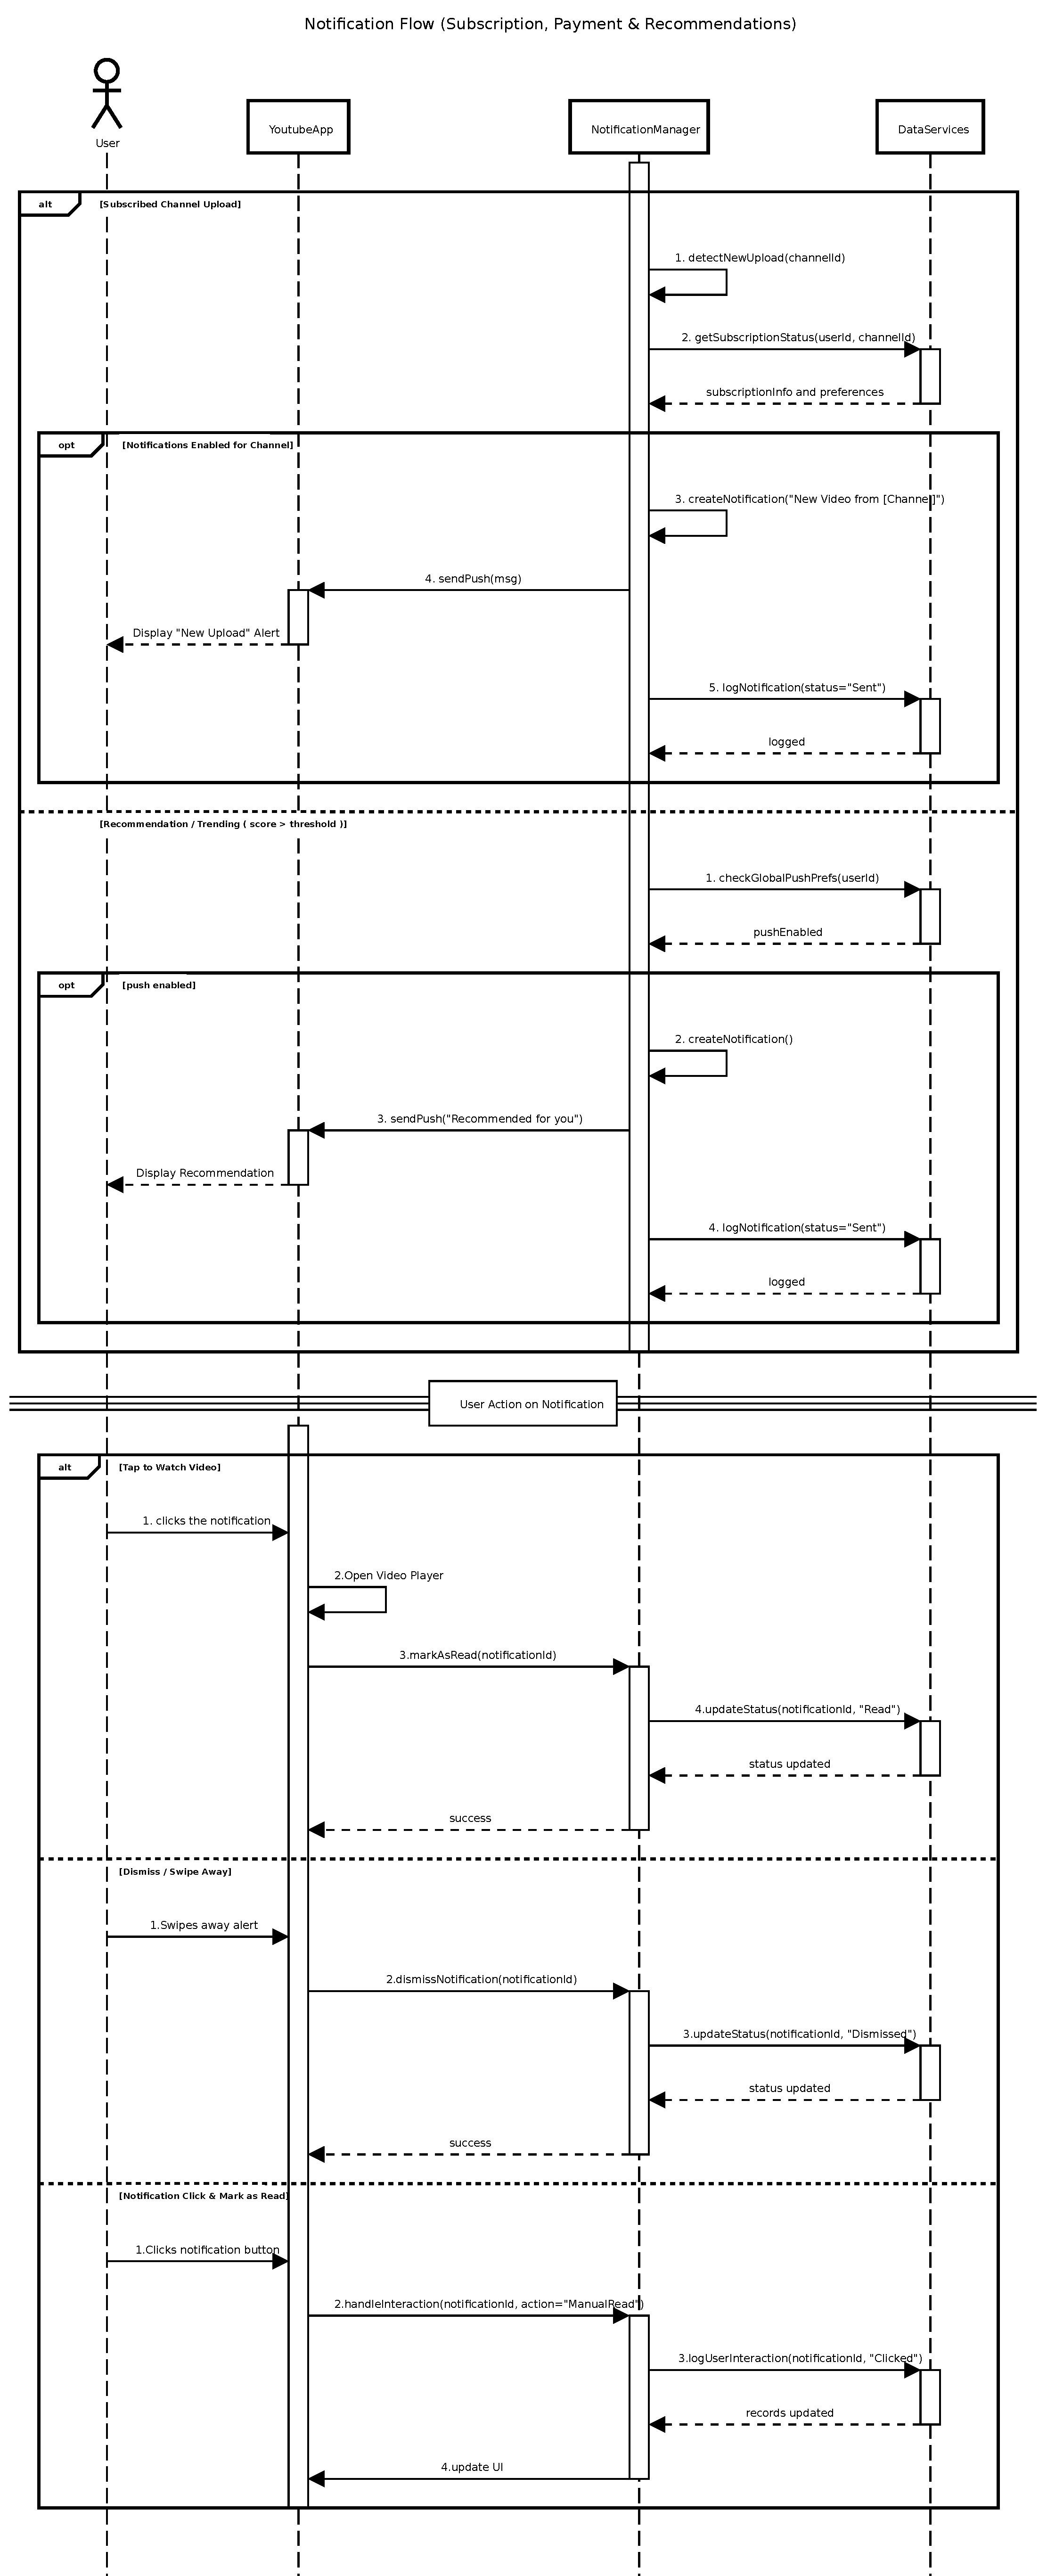
\includegraphics[width=\textwidth, height=0.85\textheight, keepaspectratio]{amit/sequence/notification_222.pdf}
    \caption{Sequence Diagram for Notification Flow}
\end{figure}

\begin{figure}[htbp]
    \centering
    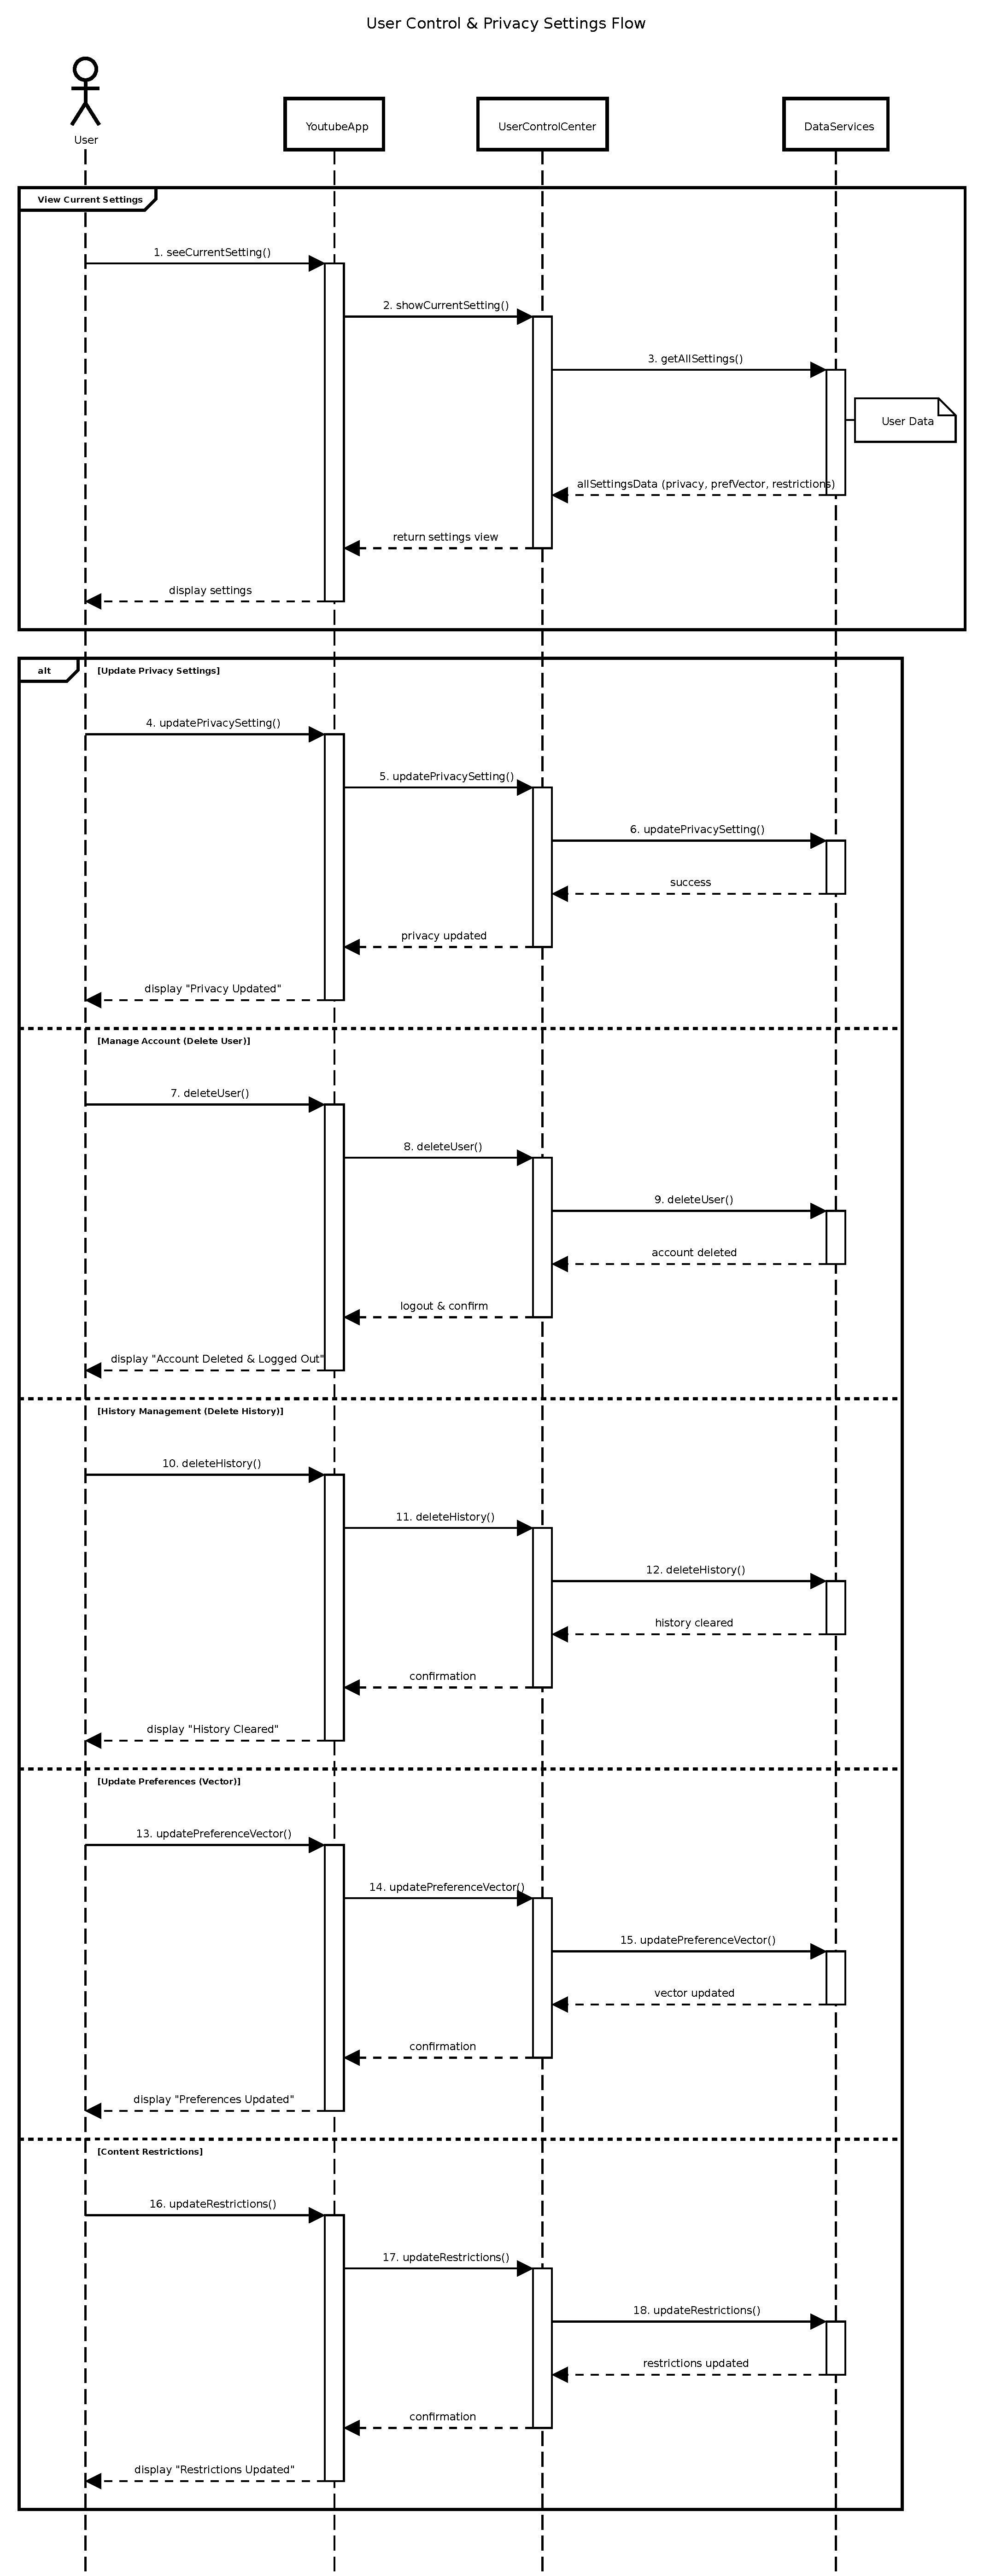
\includegraphics[width=\textwidth, height=0.85\textheight, keepaspectratio]{amit/sequence/settings_final.pdf}
    \caption{Sequence Diagram for User Control and privacy settings flow}
\end{figure}



% --- CHAPTER 8: STATE DIAGRAM ---
\chapter{State Diagram}
\textbf{Presented by: Amit Saha (2105049)} \\

\section*{Feedback Implementation}
Two updates were given for the state diagrams, 
\\1. for 8.1 (user state diagram) logged in user never got to browse video only guest could do, it was a bug, fixed now.
\\2. for 8.5 ( settiings sate diagram) there was a minor error, there was save and exit then it went to idle state but it was suggested that the only save then go to idle state, fixed now.\\
Here are the diagrams.

\vspace{1cm}

\begin{figure}[htbp]
    \centering
    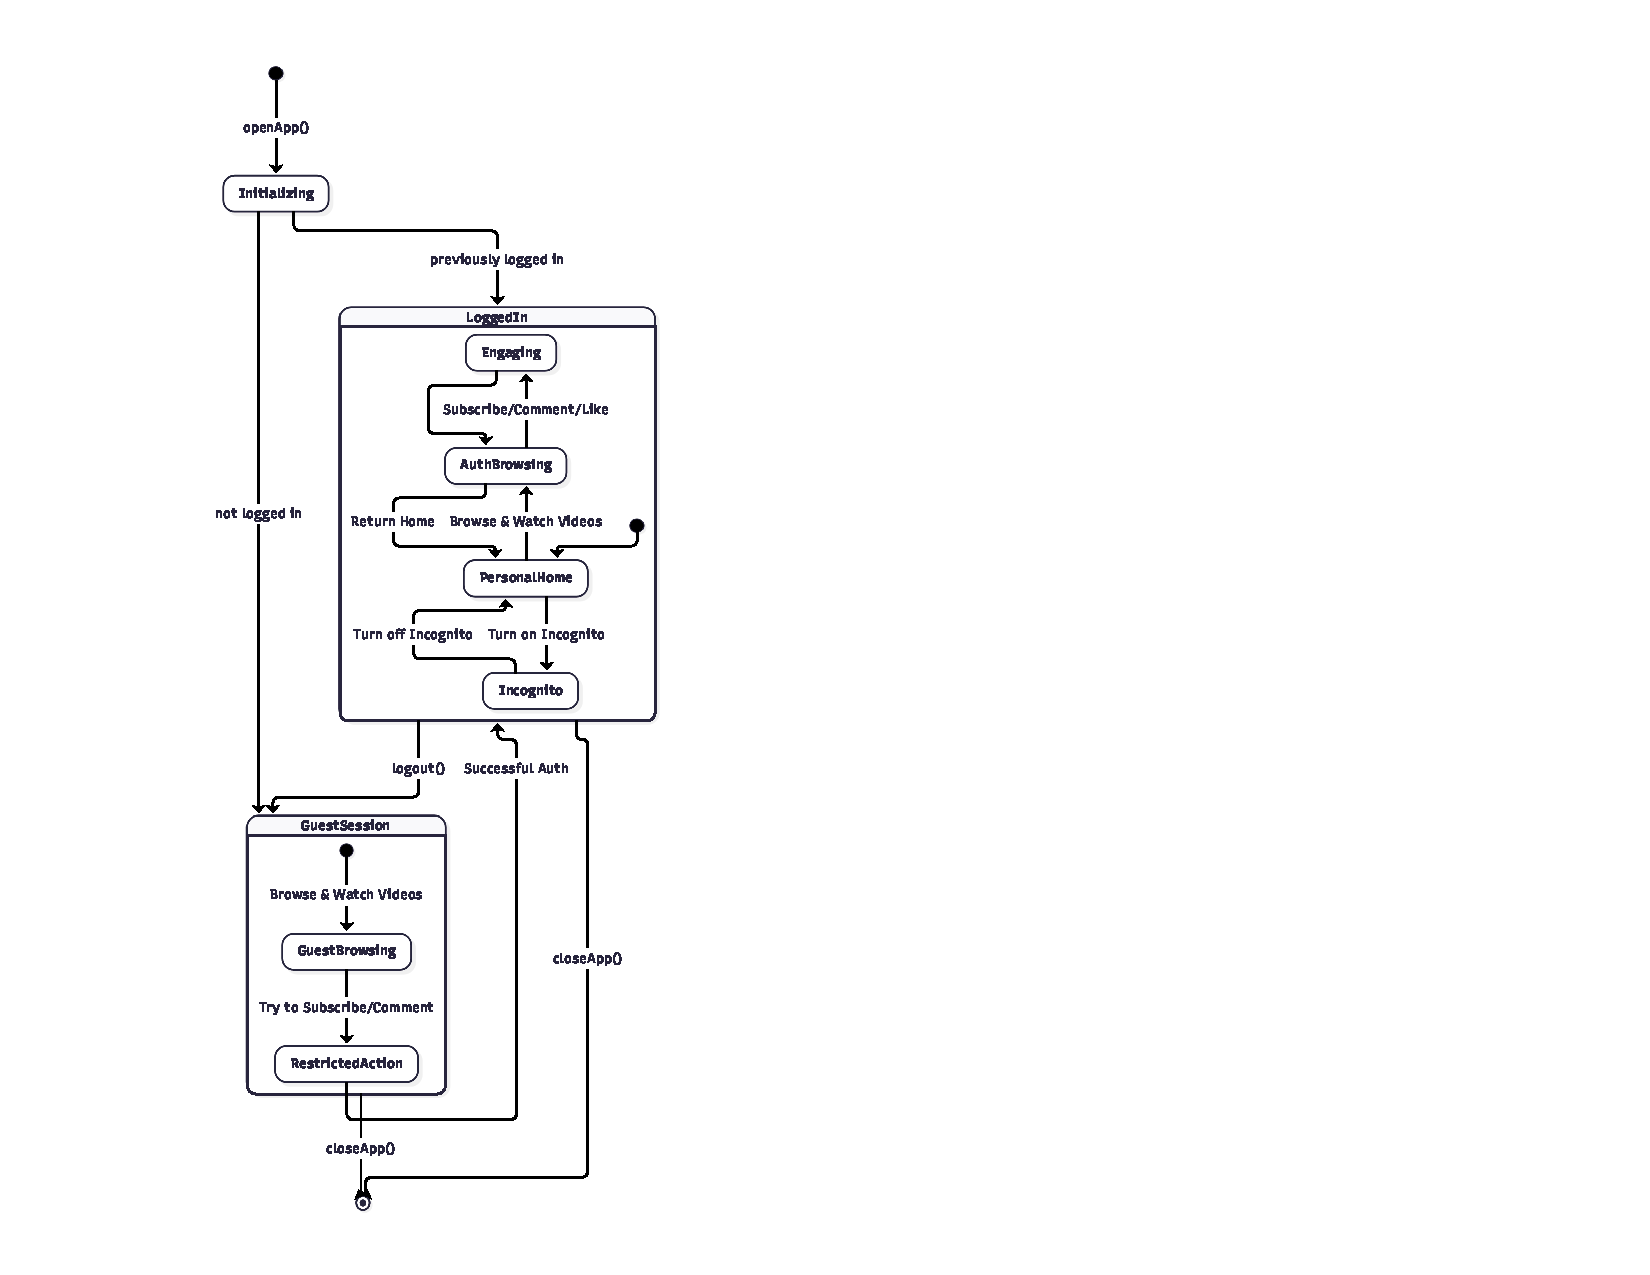
\includegraphics[width=\textwidth, height=\textheight, keepaspectratio]{amit/state/user_state_(fixed).pdf}
    \caption{Fixed state diagram for User}
\end{figure}

\begin{figure}[htbp]
    \centering
    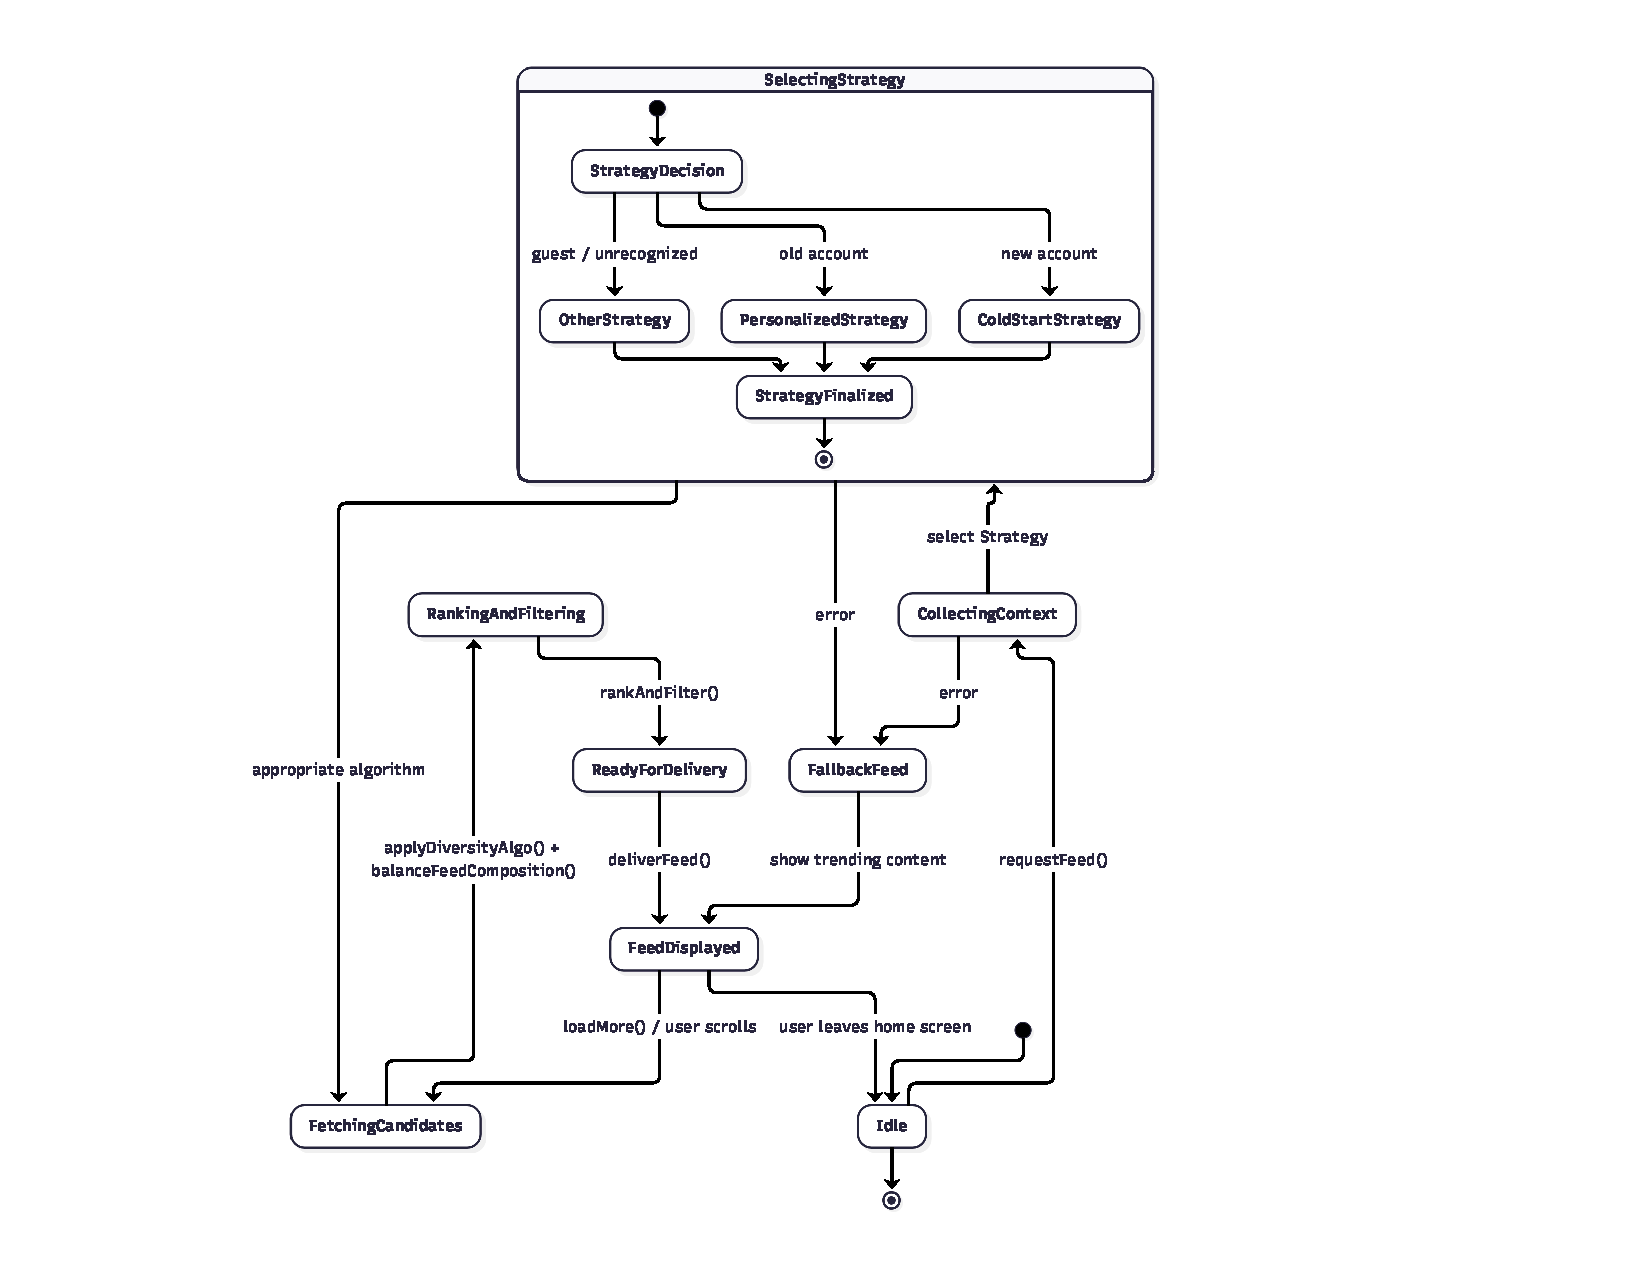
\includegraphics[width=\textwidth, height=\textheight, keepaspectratio]{amit/state/homefeed_state_222.pdf}
    \caption{State diagram for Homefeed }
\end{figure}

\begin{figure}[htbp]
    \centering
    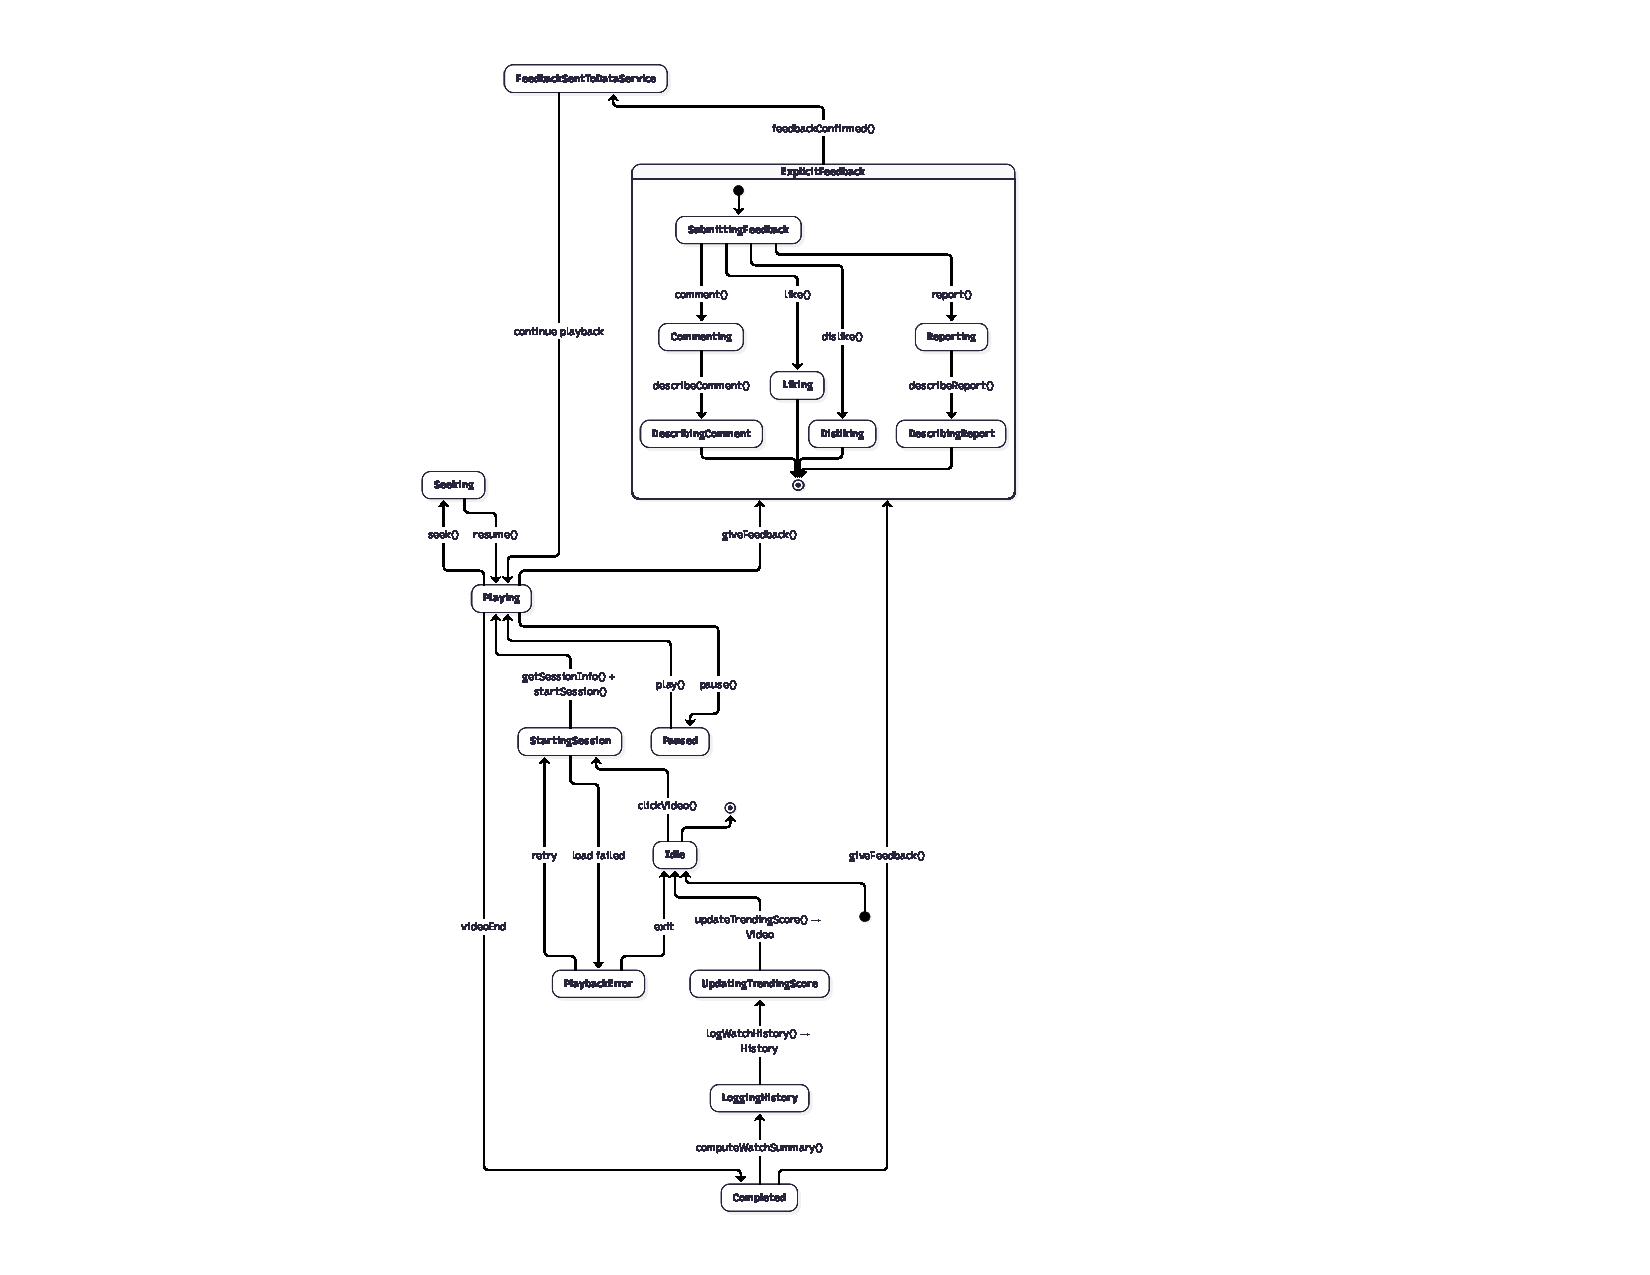
\includegraphics[width=\textwidth, height=\textheight, keepaspectratio]{amit/state/video_playback.pdf}
    \caption{State diagram for video playback and feedback}
\end{figure}

\begin{figure}[htbp]
    \centering
    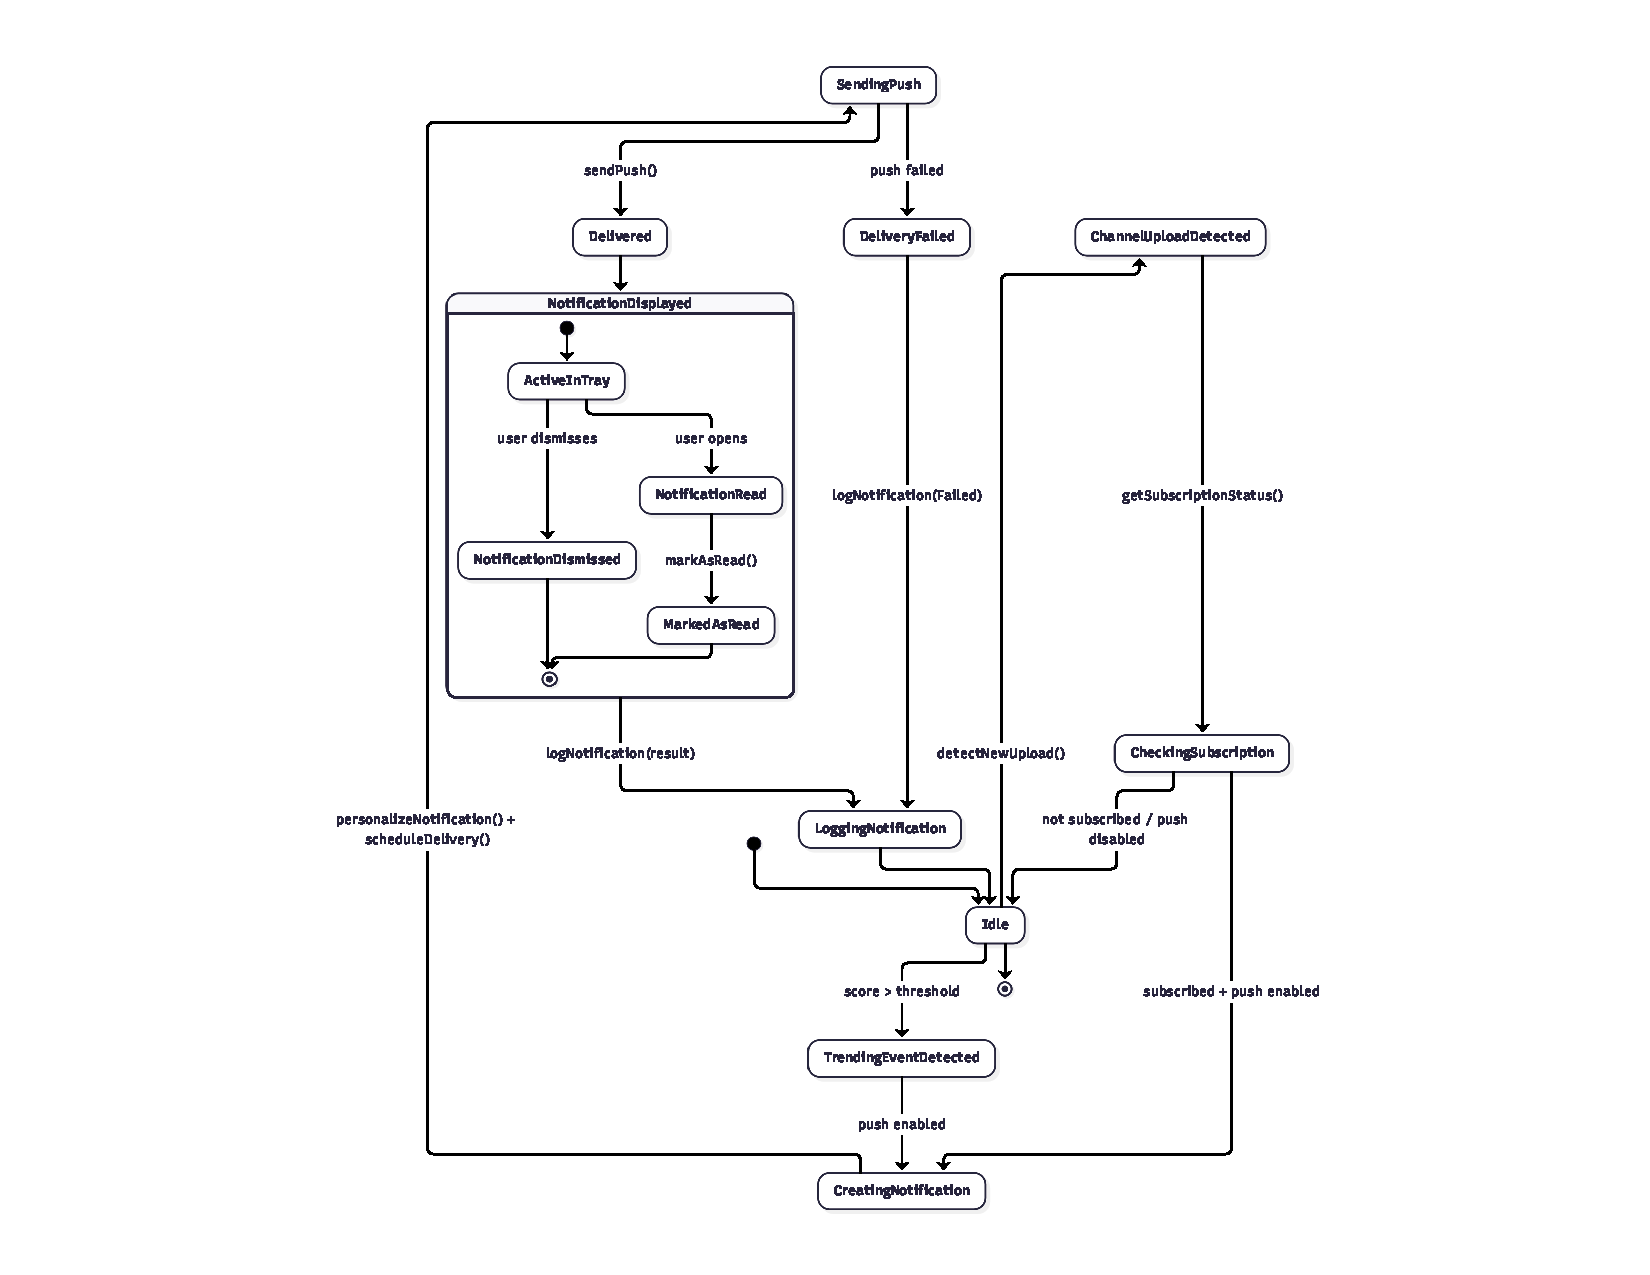
\includegraphics[width=\textwidth, height=\textheight, keepaspectratio]{amit/state/notification_state_2222.pdf}
    \caption{State diagram for notification}
\end{figure}

\begin{figure}[htbp]
    \centering
    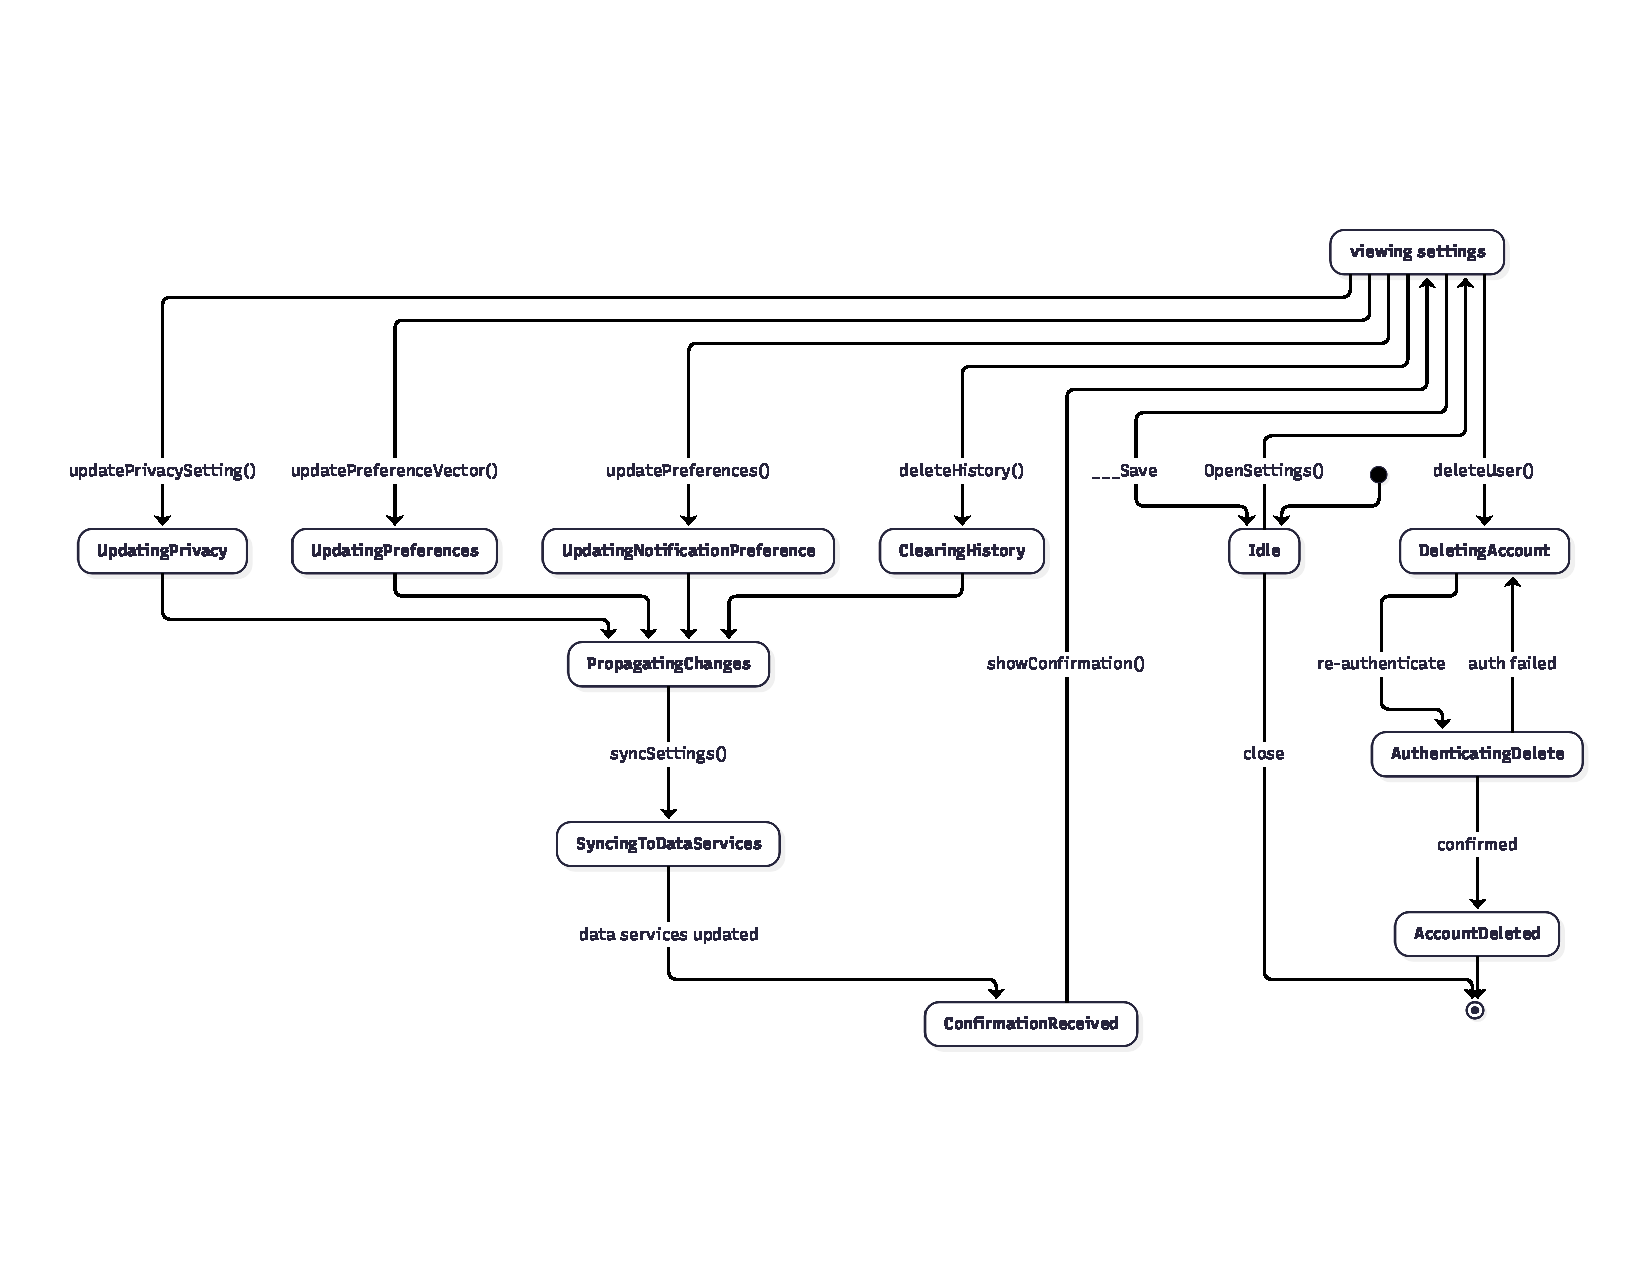
\includegraphics[width=\textwidth, height=\textheight, keepaspectratio]{amit/state/settings_state_(fixed).pdf}
    \caption{Fixed State diagram for settings update}
\end{figure}


% --- CHAPTER 9: API DOCUMENTATION ---
\chapter{API Documentation}
\textbf{Presented by: Md Abrar Jahin (2105055)} \\

\section*{Feedback Implementation}
Based on the provided feedback, the following changes were made in the API documentation:\\

\begin{itemize}
    \item \textbf{PlaylistItems Refactoring:} The standalone \texttt{/playlistItems} resource was removed. Playlist item management is now nested under the parent playlist resource as \\ \texttt{/playlists/\{playlistId\}/items} and \texttt{/playlists/\{playlistId\}/items/\{itemId\}},\\ enforcing proper REST resource hierarchy.

    \item \textbf{Video Schema Cleanup:} Video duration was added to the \texttt{Video} snippet object under the \texttt{GET /videos} API hierarchy as \texttt{durationSeconds}. Redundant \texttt{likeCount} and \texttt{dislikeCount} fields were removed from \texttt{Video.statistics} and kept exclusively under\\ \texttt{GET /videos/\{videoId\}/stats}.
\end{itemize}

The full API Documentation is provided in the following pages.
\newpage

{

\begin{figure}[htbp]
    \centering
    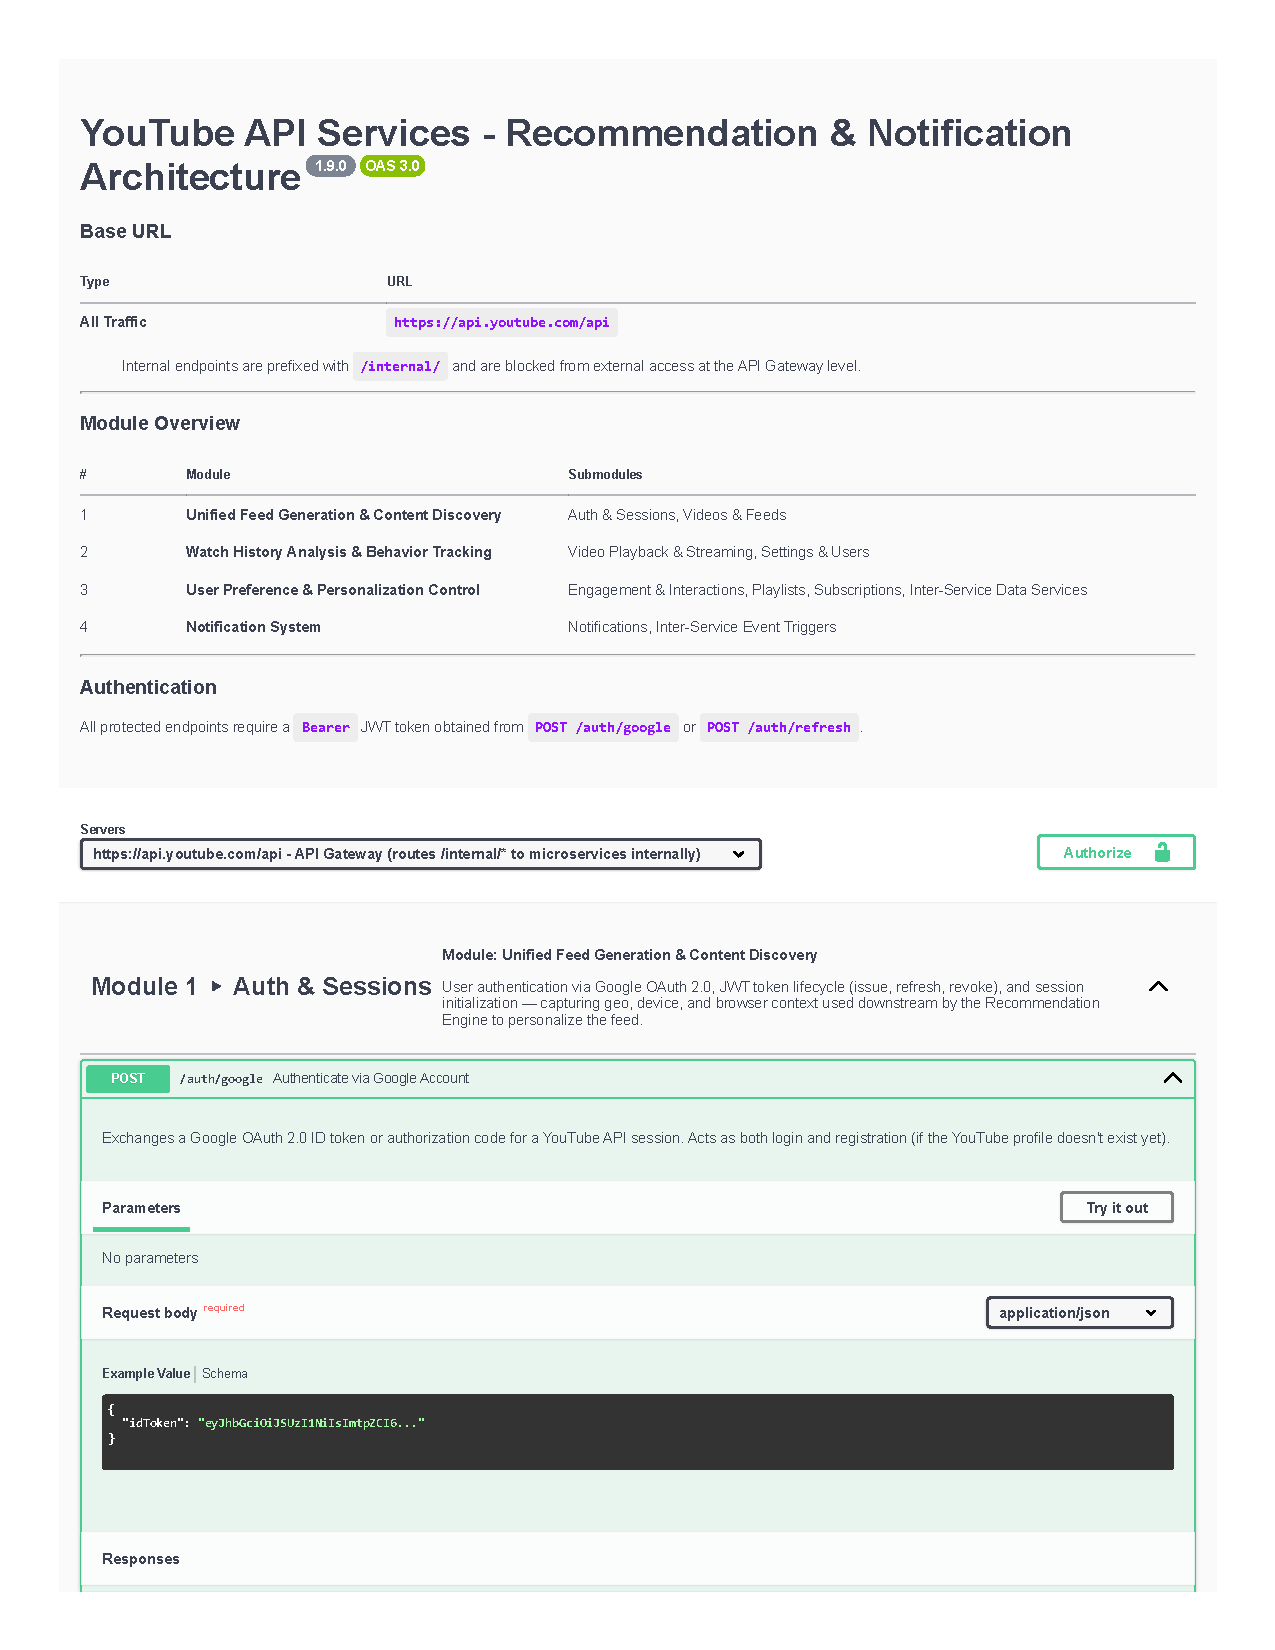
\includegraphics[width=\textwidth, height=\textheight, keepaspectratio, page=1]{abrar/API_Documentation.pdf}
\end{figure}

\begin{figure}[htbp]
    \centering
    \includegraphics[width=\textwidth, height=\textheight, keepaspectratio, page=2]{abrar/API_Documentation.pdf}
\end{figure}

\begin{figure}[htbp]
    \centering
    \includegraphics[width=\textwidth, height=\textheight, keepaspectratio, page=3]{abrar/API_Documentation.pdf}
\end{figure}

\begin{figure}[htbp]
    \centering
    \includegraphics[width=\textwidth, height=\textheight, keepaspectratio, page=4]{abrar/API_Documentation.pdf}
\end{figure}

\begin{figure}[htbp]
    \centering
    \includegraphics[width=\textwidth, height=\textheight, keepaspectratio, page=5]{abrar/API_Documentation.pdf}
\end{figure}

\begin{figure}[htbp]
    \centering
    \includegraphics[width=\textwidth, height=\textheight, keepaspectratio, page=6]{abrar/API_Documentation.pdf}
\end{figure}

\begin{figure}[htbp]
    \centering
    \includegraphics[width=\textwidth, height=\textheight, keepaspectratio, page=7]{abrar/API_Documentation.pdf}
\end{figure}

\begin{figure}[htbp]
    \centering
    \includegraphics[width=\textwidth, height=\textheight, keepaspectratio, page=8]{abrar/API_Documentation.pdf}
\end{figure}

\begin{figure}[htbp]
    \centering
    \includegraphics[width=\textwidth, height=\textheight, keepaspectratio, page=9]{abrar/API_Documentation.pdf}
\end{figure}

\begin{figure}[htbp]
    \centering
    \includegraphics[width=\textwidth, height=\textheight, keepaspectratio, page=10]{abrar/API_Documentation.pdf}
\end{figure}

\begin{figure}[htbp]
    \centering
    \includegraphics[width=\textwidth, height=\textheight, keepaspectratio, page=11]{abrar/API_Documentation.pdf}
\end{figure}

\begin{figure}[htbp]
    \centering
    \includegraphics[width=\textwidth, height=\textheight, keepaspectratio, page=12]{abrar/API_Documentation.pdf}
\end{figure}

\begin{figure}[htbp]
    \centering
    \includegraphics[width=\textwidth, height=\textheight, keepaspectratio, page=13]{abrar/API_Documentation.pdf}
\end{figure}

\begin{figure}[htbp]
    \centering
    \includegraphics[width=\textwidth, height=\textheight, keepaspectratio, page=14]{abrar/API_Documentation.pdf}
\end{figure}

\begin{figure}[htbp]
    \centering
    \includegraphics[width=\textwidth, height=\textheight, keepaspectratio, page=15]{abrar/API_Documentation.pdf}
\end{figure}

\begin{figure}[htbp]
    \centering
    \includegraphics[width=\textwidth, height=\textheight, keepaspectratio, page=16]{abrar/API_Documentation.pdf}
\end{figure}

\begin{figure}[htbp]
    \centering
    \includegraphics[width=\textwidth, height=\textheight, keepaspectratio, page=17]{abrar/API_Documentation.pdf}
\end{figure}

\begin{figure}[htbp]
    \centering
    \includegraphics[width=\textwidth, height=\textheight, keepaspectratio, page=18]{abrar/API_Documentation.pdf}
\end{figure}

\begin{figure}[htbp]
    \centering
    \includegraphics[width=\textwidth, height=\textheight, keepaspectratio, page=19]{abrar/API_Documentation.pdf}
\end{figure}

\begin{figure}[htbp]
    \centering
    \includegraphics[width=\textwidth, height=\textheight, keepaspectratio, page=20]{abrar/API_Documentation.pdf}
\end{figure}

\begin{figure}[htbp]
    \centering
    \includegraphics[width=\textwidth, height=\textheight, keepaspectratio, page=21]{abrar/API_Documentation.pdf}
\end{figure}

\begin{figure}[htbp]
    \centering
    \includegraphics[width=\textwidth, height=\textheight, keepaspectratio, page=22]{abrar/API_Documentation.pdf}
\end{figure}

\begin{figure}[htbp]
    \centering
    \includegraphics[width=\textwidth, height=\textheight, keepaspectratio, page=23]{abrar/API_Documentation.pdf}
\end{figure}

\begin{figure}[htbp]
    \centering
    \includegraphics[width=\textwidth, height=\textheight, keepaspectratio, page=24]{abrar/API_Documentation.pdf}
\end{figure}

\begin{figure}[htbp]
    \centering
    \includegraphics[width=\textwidth, height=\textheight, keepaspectratio, page=25]{abrar/API_Documentation.pdf}
\end{figure}

\begin{figure}[htbp]
    \centering
    \includegraphics[width=\textwidth, height=\textheight, keepaspectratio, page=26]{abrar/API_Documentation.pdf}
\end{figure}

\begin{figure}[htbp]
    \centering
    \includegraphics[width=\textwidth, height=\textheight, keepaspectratio, page=27]{abrar/API_Documentation.pdf}
\end{figure}

\begin{figure}[htbp]
    \centering
    \includegraphics[width=\textwidth, height=\textheight, keepaspectratio, page=28]{abrar/API_Documentation.pdf}
\end{figure}

\begin{figure}[htbp]
    \centering
    \includegraphics[width=\textwidth, height=\textheight, keepaspectratio, page=29]{abrar/API_Documentation.pdf}
\end{figure}

\begin{figure}[htbp]
    \centering
    \includegraphics[width=\textwidth, height=\textheight, keepaspectratio, page=30]{abrar/API_Documentation.pdf}
\end{figure}

\begin{figure}[htbp]
    \centering
    \includegraphics[width=\textwidth, height=\textheight, keepaspectratio, page=31]{abrar/API_Documentation.pdf}
\end{figure}

\begin{figure}[htbp]
    \centering
    \includegraphics[width=\textwidth, height=\textheight, keepaspectratio, page=32]{abrar/API_Documentation.pdf}
\end{figure}

\begin{figure}[htbp]
    \centering
    \includegraphics[width=\textwidth, height=\textheight, keepaspectratio, page=33]{abrar/API_Documentation.pdf}
\end{figure}

\begin{figure}[htbp]
    \centering
    \includegraphics[width=\textwidth, height=\textheight, keepaspectratio, page=34]{abrar/API_Documentation.pdf}
\end{figure}

\begin{figure}[htbp]
    \centering
    \includegraphics[width=\textwidth, height=\textheight, keepaspectratio, page=35]{abrar/API_Documentation.pdf}
\end{figure}

\begin{figure}[htbp]
    \centering
    \includegraphics[width=\textwidth, height=\textheight, keepaspectratio, page=36]{abrar/API_Documentation.pdf}
\end{figure}

\begin{figure}[htbp]
    \centering
    \includegraphics[width=\textwidth, height=\textheight, keepaspectratio, page=37]{abrar/API_Documentation.pdf}
\end{figure}

\begin{figure}[htbp]
    \centering
    \includegraphics[width=\textwidth, height=\textheight, keepaspectratio, page=38]{abrar/API_Documentation.pdf}
\end{figure}
}

% --- CHAPTER 10: FEATURE IMPLEMENTATION ---
\chapter{Feature Implementation}

\section{Feature Overview}
\textbf{Name:} Homefeed, Content Discovery (Video Playback), and Recommendation Engine. \\
\textbf{Description:} A highly personalized content delivery system that transitions seamlessly from a Cold Start strategy (for Guest Users) to a vector-based Personalized Feed (for Registered Users) using a 4-Bucket balancing algorithm.

\section{Project Links}
\begin{itemize}
    \item \textbf{GitHub Repository:} \url{https://github.com/Abhishek12105021/CSE-326-ISD-Sessional}
    \item \textbf{Deployed Project:} \url{https://youtube-clone-frontend-olive.vercel.app}
\end{itemize}

\section{Application Screenshots}

\begin{figure}[H]
  \centering
    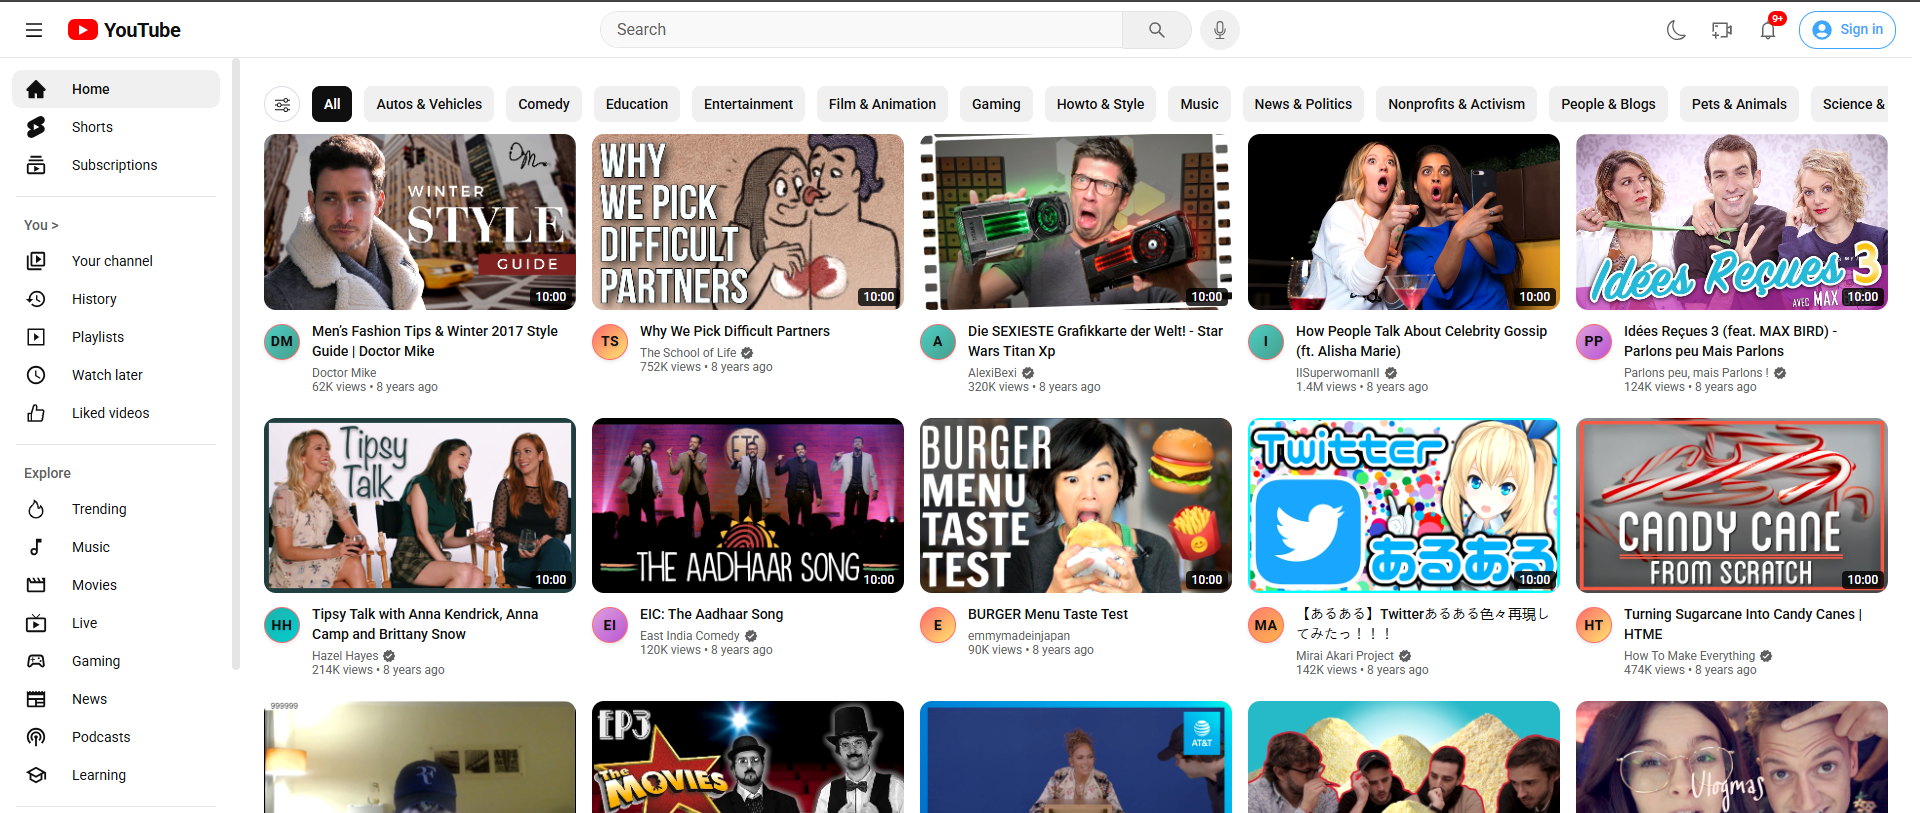
\includegraphics[width=0.9\textwidth]{img-App/Home-Guest.png}
    \vspace{0.3cm}\\
    The guest user homefeed displaying globally trending videos across multiple categories with the tag-based filter bar at the top, powered by the Cold Start exploration strategy.
    \caption{Guest User Homefeed}
    \label{fig:app_home_guest}
\end{figure}

\begin{figure}[H]
  \centering
    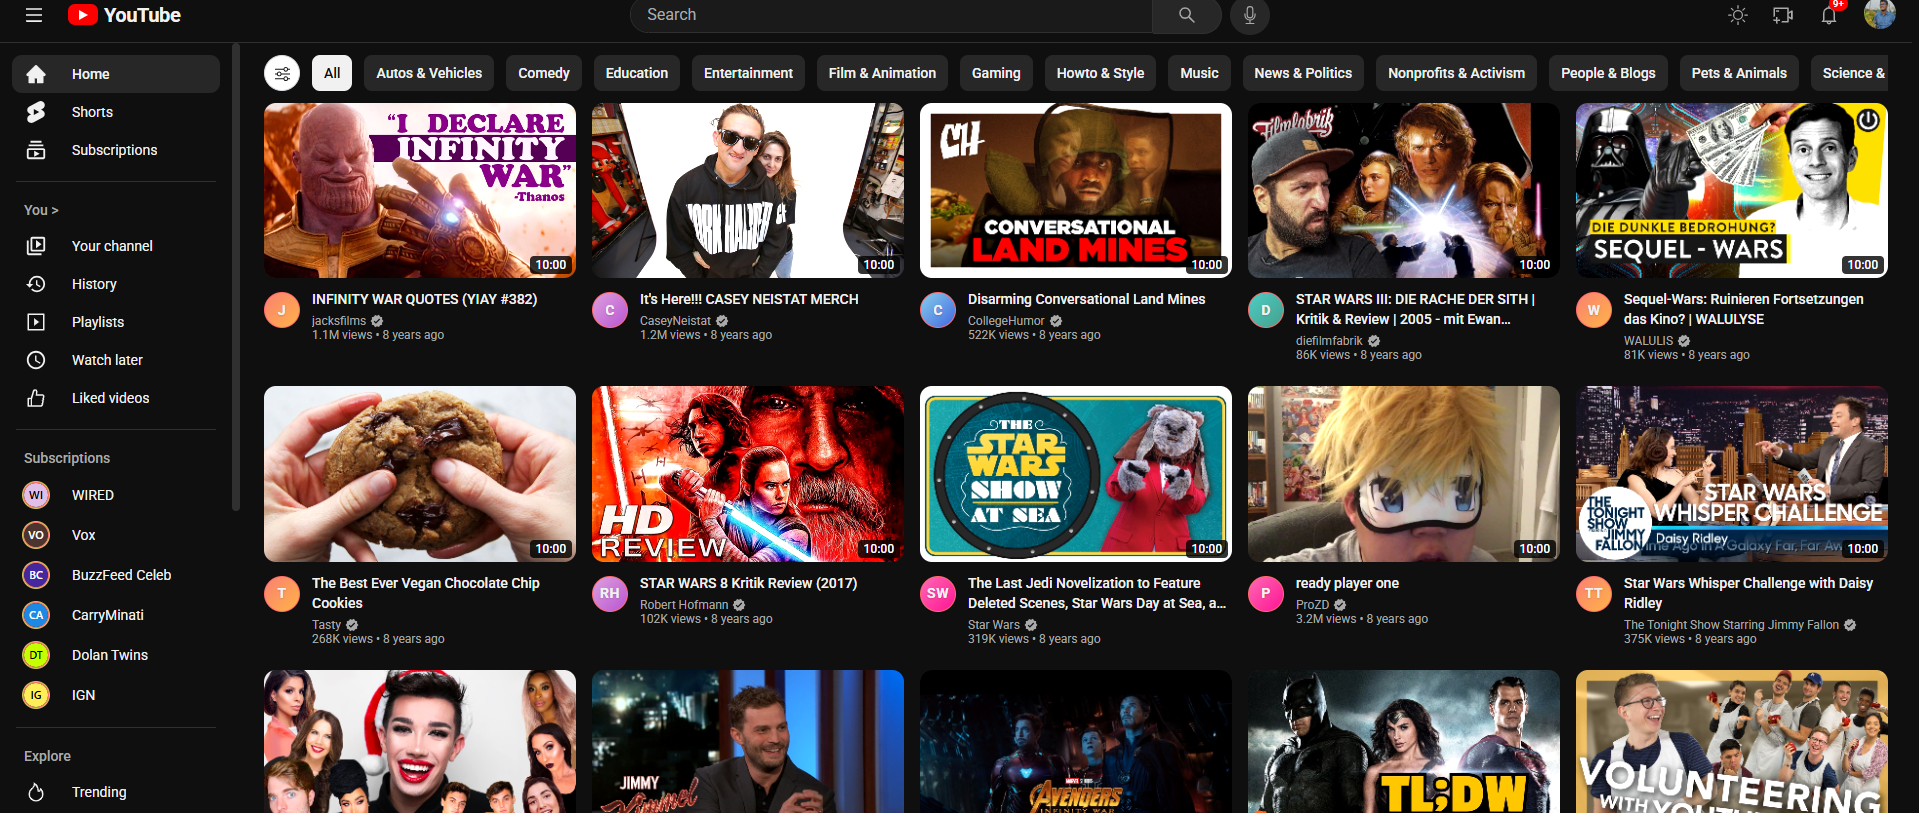
\includegraphics[width=0.9\textwidth]{img-App/Home-Personalized.png}
    \vspace{0.3cm}\\
    The personalized homefeed for a signed-in user in dark mode, showing semantically recommended videos generated by the 4-Bucket Recommendation Strategy based on the user's watch history and taste vector.
    \caption{Personalized Homefeed (Signed-In User)}
    \label{fig:app_home_personalized}
\end{figure}

\begin{figure}[H]
  \centering
    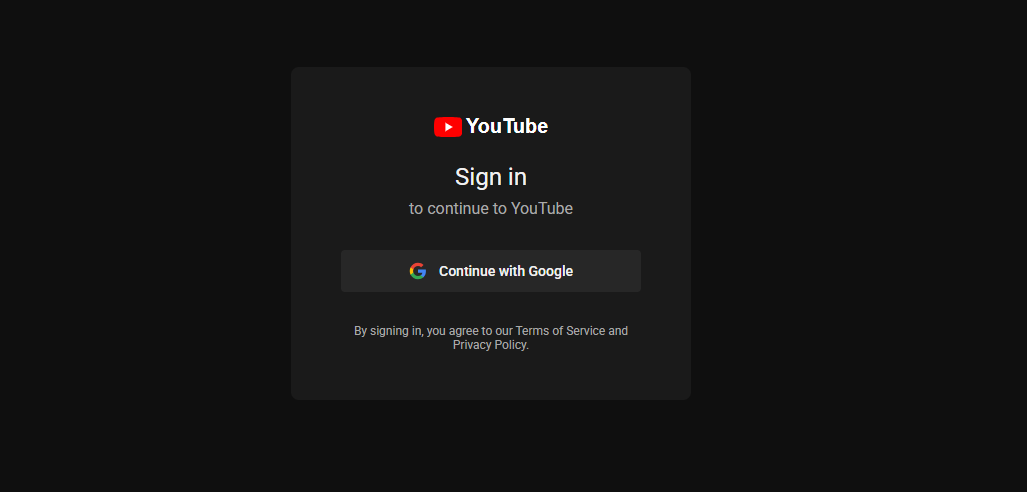
\includegraphics[width=0.9\textwidth]{img-App/SignIn.png}
    \vspace{0.3cm}\\
    The sign-in page prompting users to authenticate via Google OAuth, with links to the Terms of Service and Privacy Policy.
    \caption{Sign In Page}
    \label{fig:app_signin}
\end{figure}

\begin{figure}[H]
  \centering
    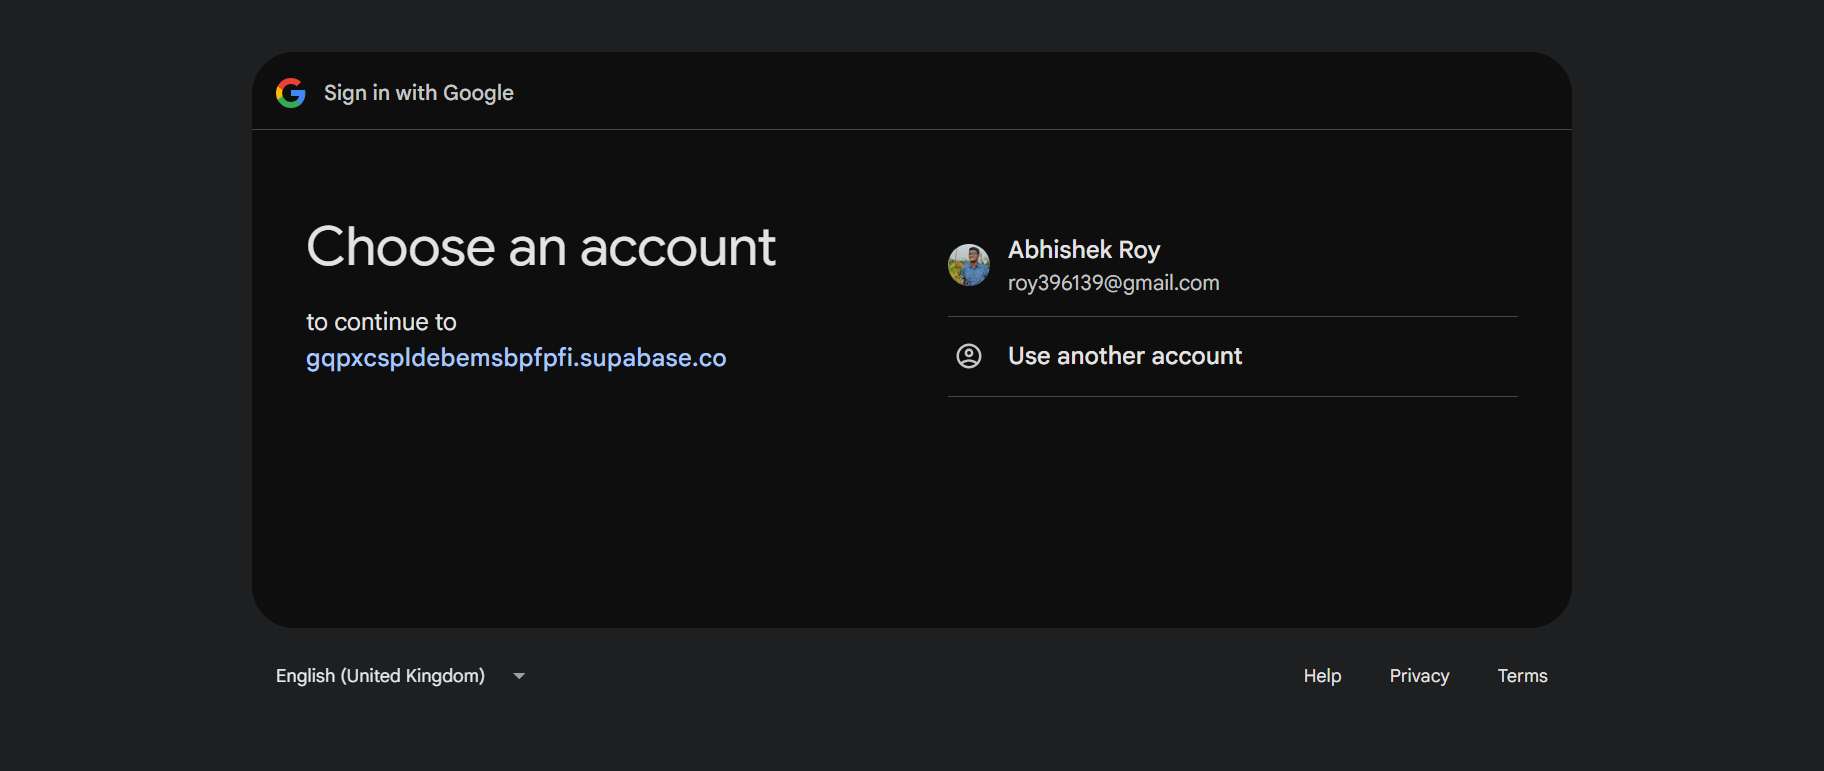
\includegraphics[width=0.9\textwidth]{img-App/SignIn-Google.png}
    \vspace{0.3cm}\\
    The Google OAuth account selection screen, redirecting users to the Supabase authentication endpoint to complete the sign-in flow.
    \caption{Google OAuth Account Selection}
    \label{fig:app_signin_google}
\end{figure}

\begin{figure}[H]
  \centering
    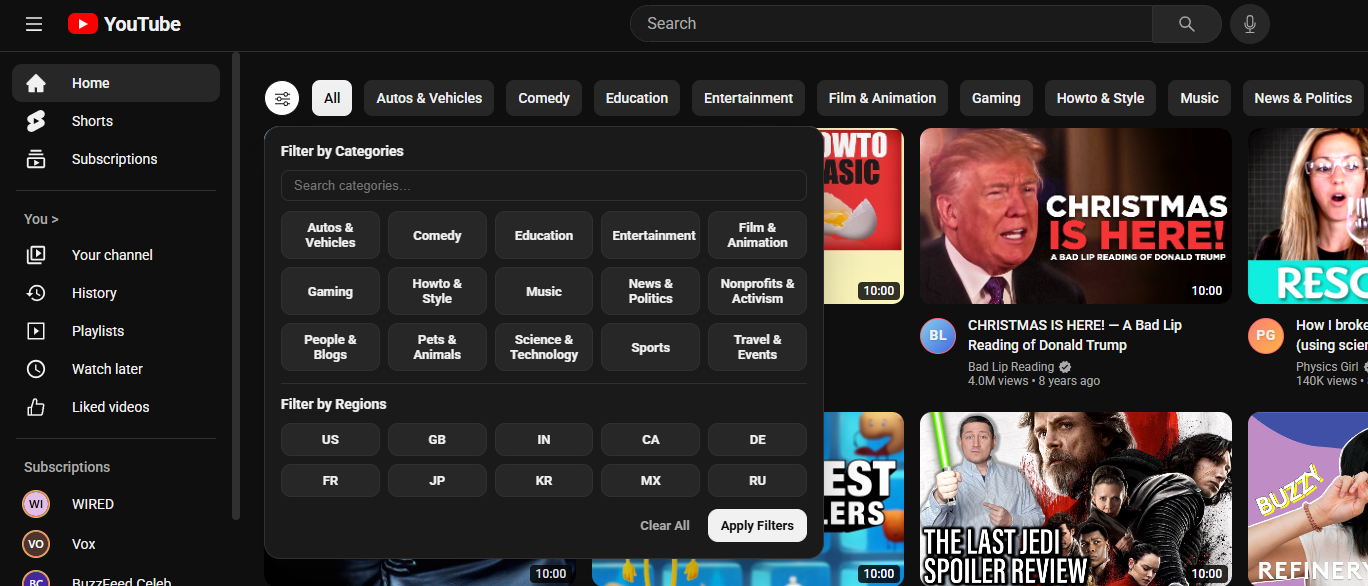
\includegraphics[width=0.9\textwidth]{img-App/Filter.png}
    \vspace{0.3cm}\\
    The expanded filter panel on the homefeed, displaying category-based and region-based filtering options allowing users to refine their content discovery.
    \caption{Homefeed Filter Panel}
    \label{fig:app_filter}
\end{figure}

\begin{figure}[H]
  \centering
    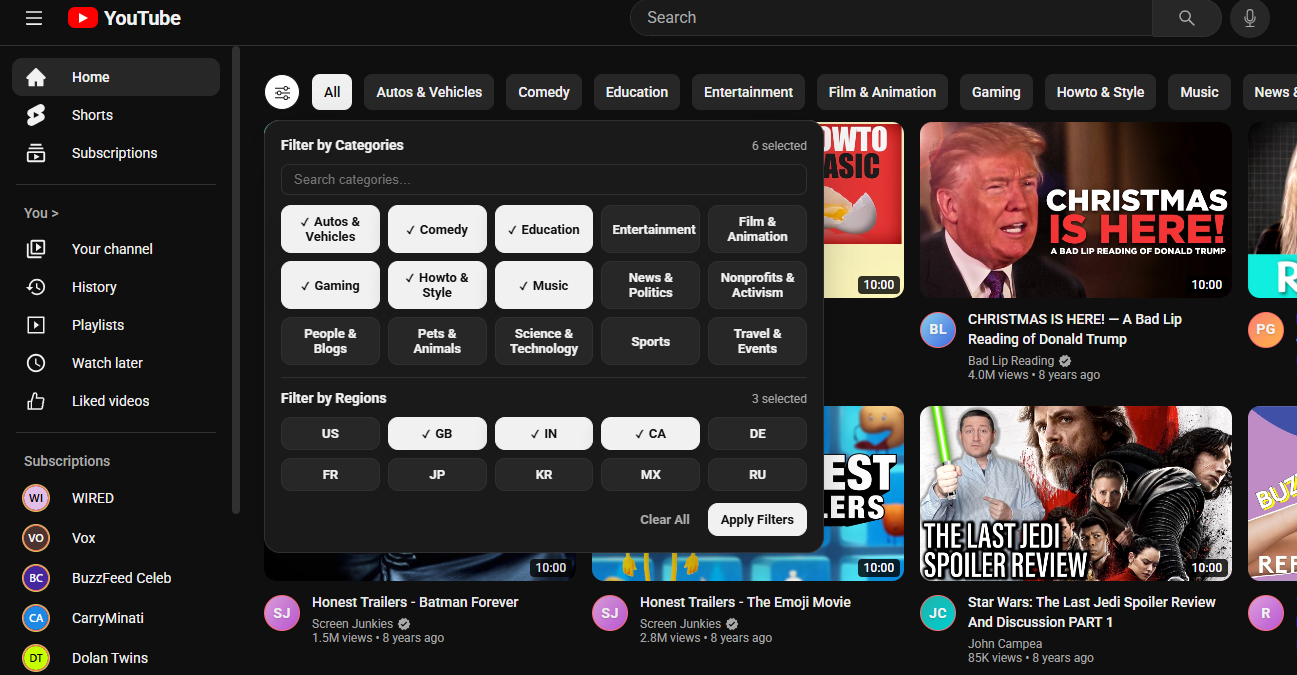
\includegraphics[width=0.9\textwidth]{img-App/Filter-Select.png}
    \vspace{0.3cm}\\
    The filter panel with multiple categories and regions actively selected, demonstrating the multi-select functionality before applying the filters.
    \caption{Filter Panel with Active Selections}
    \label{fig:app_filter_select}
\end{figure}

\begin{figure}[H]
  \centering
    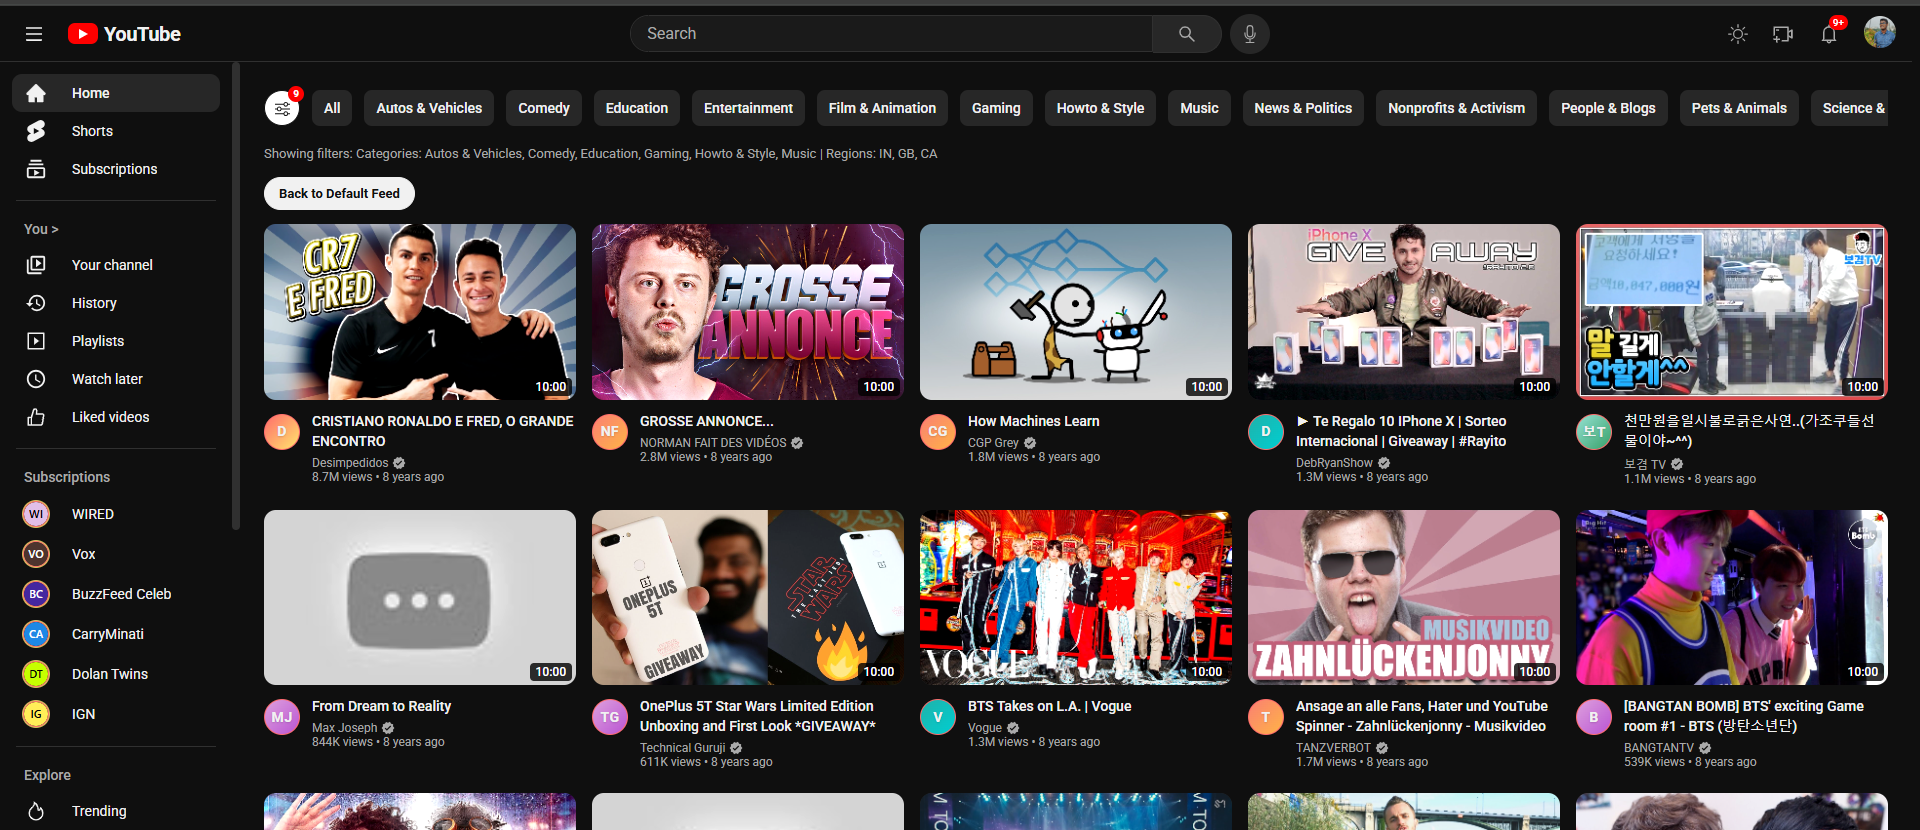
\includegraphics[width=0.9\textwidth]{img-App/Filter-Apply.png}
    \vspace{0.3cm}\\
    The homefeed after applying category and region filters, showing a curated grid of videos matching the selected criteria with a ``Back to Default Feed'' option to reset.
    \caption{Filtered Homefeed Results}
    \label{fig:app_filter_apply}
\end{figure}

\begin{figure}[H]
  \centering
    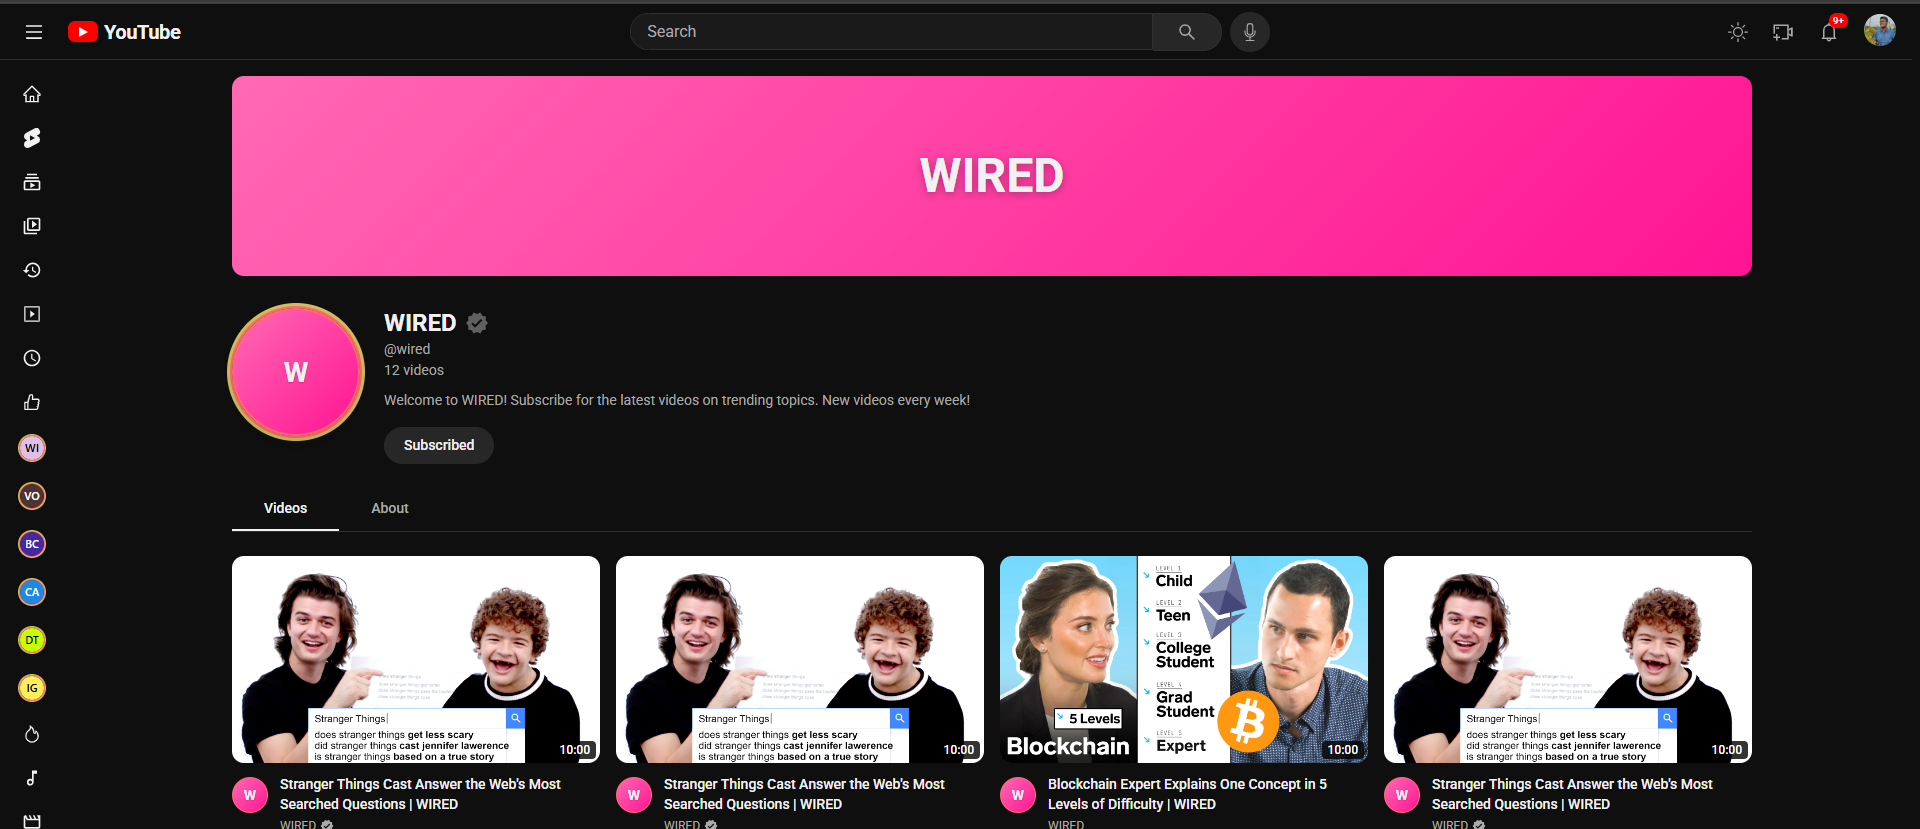
\includegraphics[width=0.9\textwidth]{img-App/Channel.png}
    \vspace{0.3cm}\\
    A channel page displaying the channel banner, profile avatar, subscriber count, and a grid of uploaded videos with the Subscribe button and navigation tabs.
    \caption{Channel Page}
    \label{fig:app_channel}
\end{figure}

\begin{figure}[H]
  \centering
    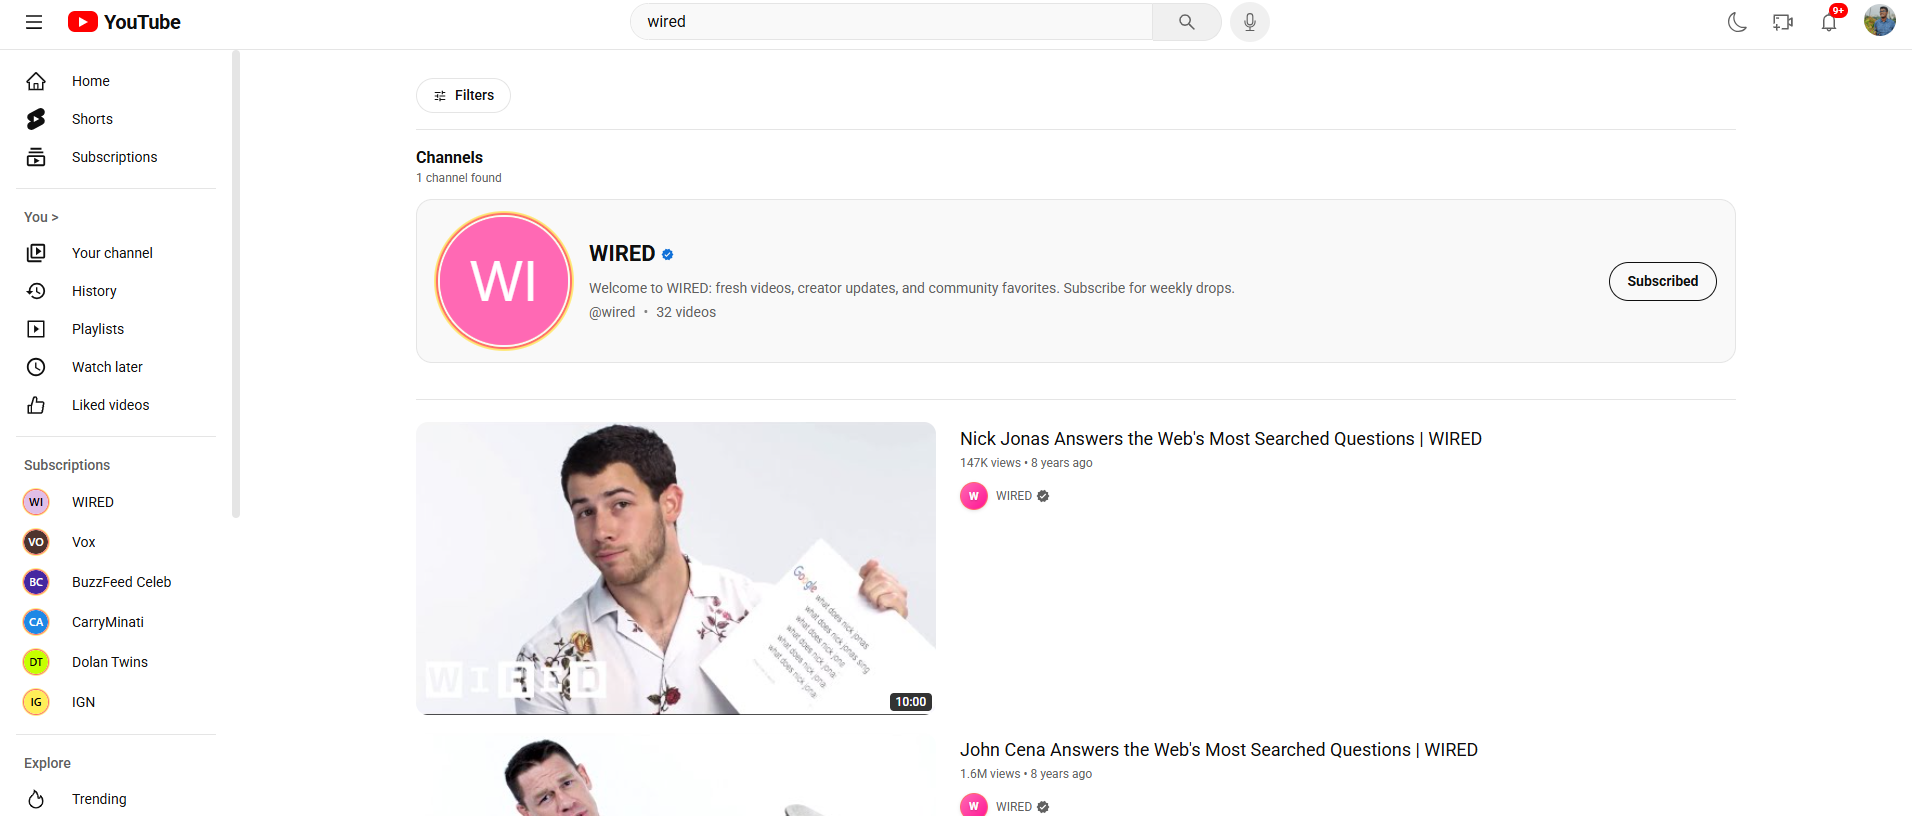
\includegraphics[width=0.9\textwidth]{img-App/Search-Channel.png}
    \vspace{0.3cm}\\
    Search results for a channel query in light mode, showing the matched channel card with subscription status and its associated video listings below.
    \caption{Search Results -- Channel Match}
    \label{fig:app_search_channel}
\end{figure}

\begin{figure}[H]
  \centering
    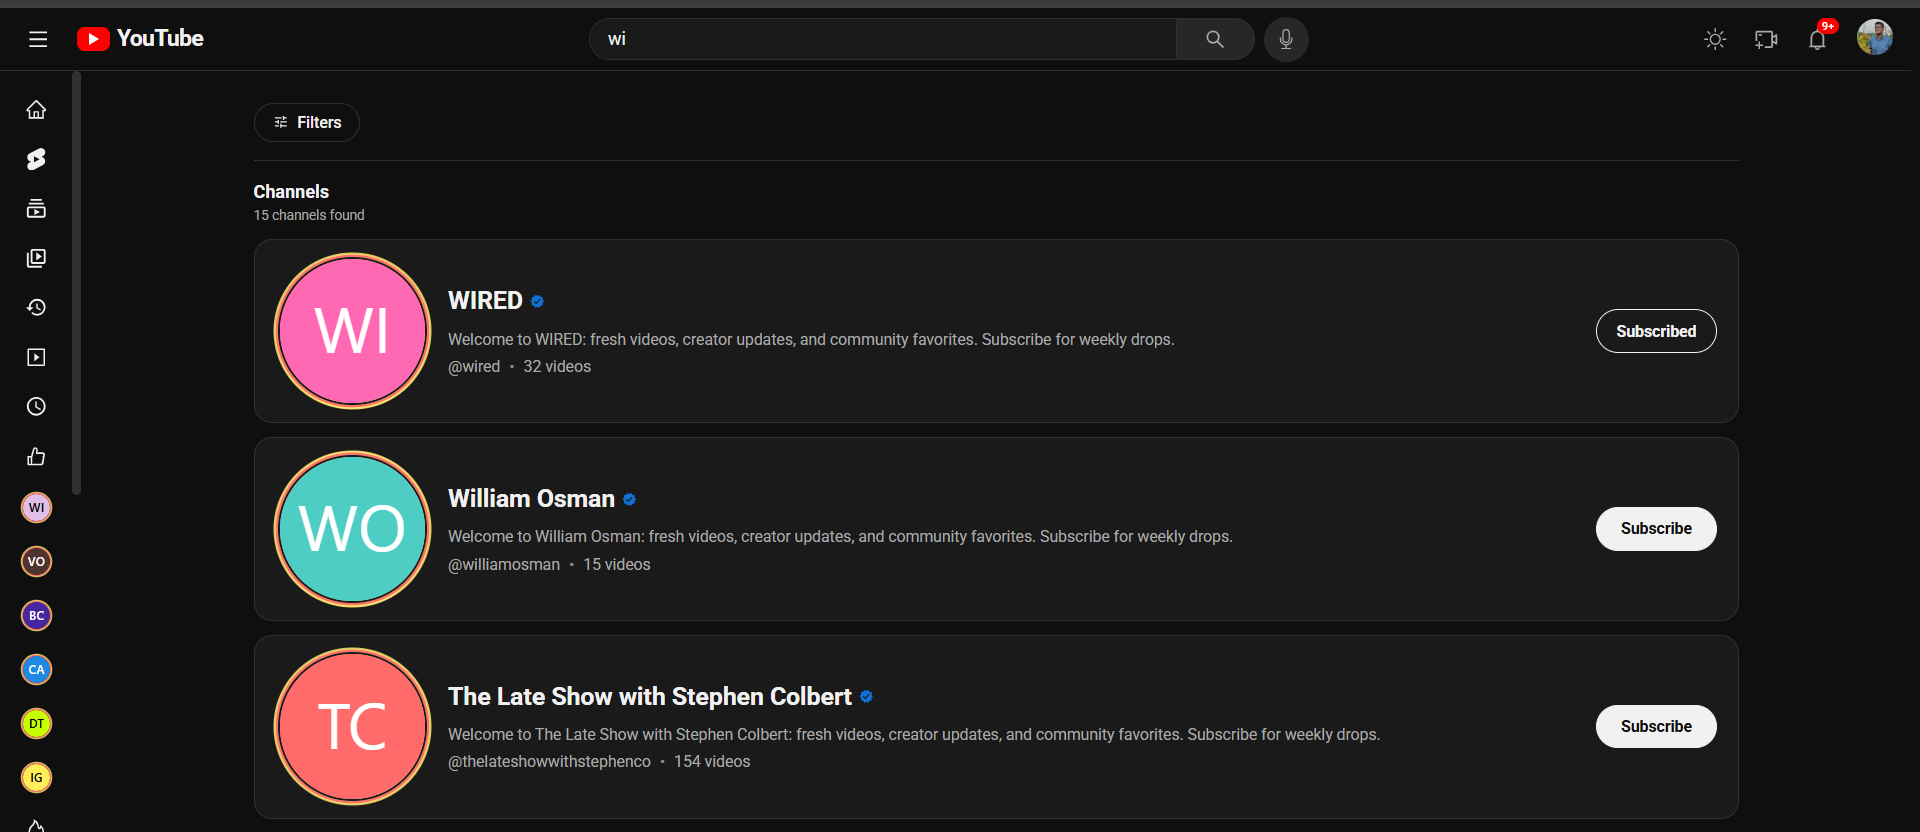
\includegraphics[width=0.9\textwidth]{img-App/Search-keyword-channel.png}
    \vspace{0.3cm}\\
    Keyword-based search results displaying multiple matching channels ranked by relevance, each showing their description, video count, and subscription status.
    \caption{Search Results -- Keyword Channel Matches}
    \label{fig:app_search_keyword_channel}
\end{figure}

\begin{figure}[H]
  \centering
    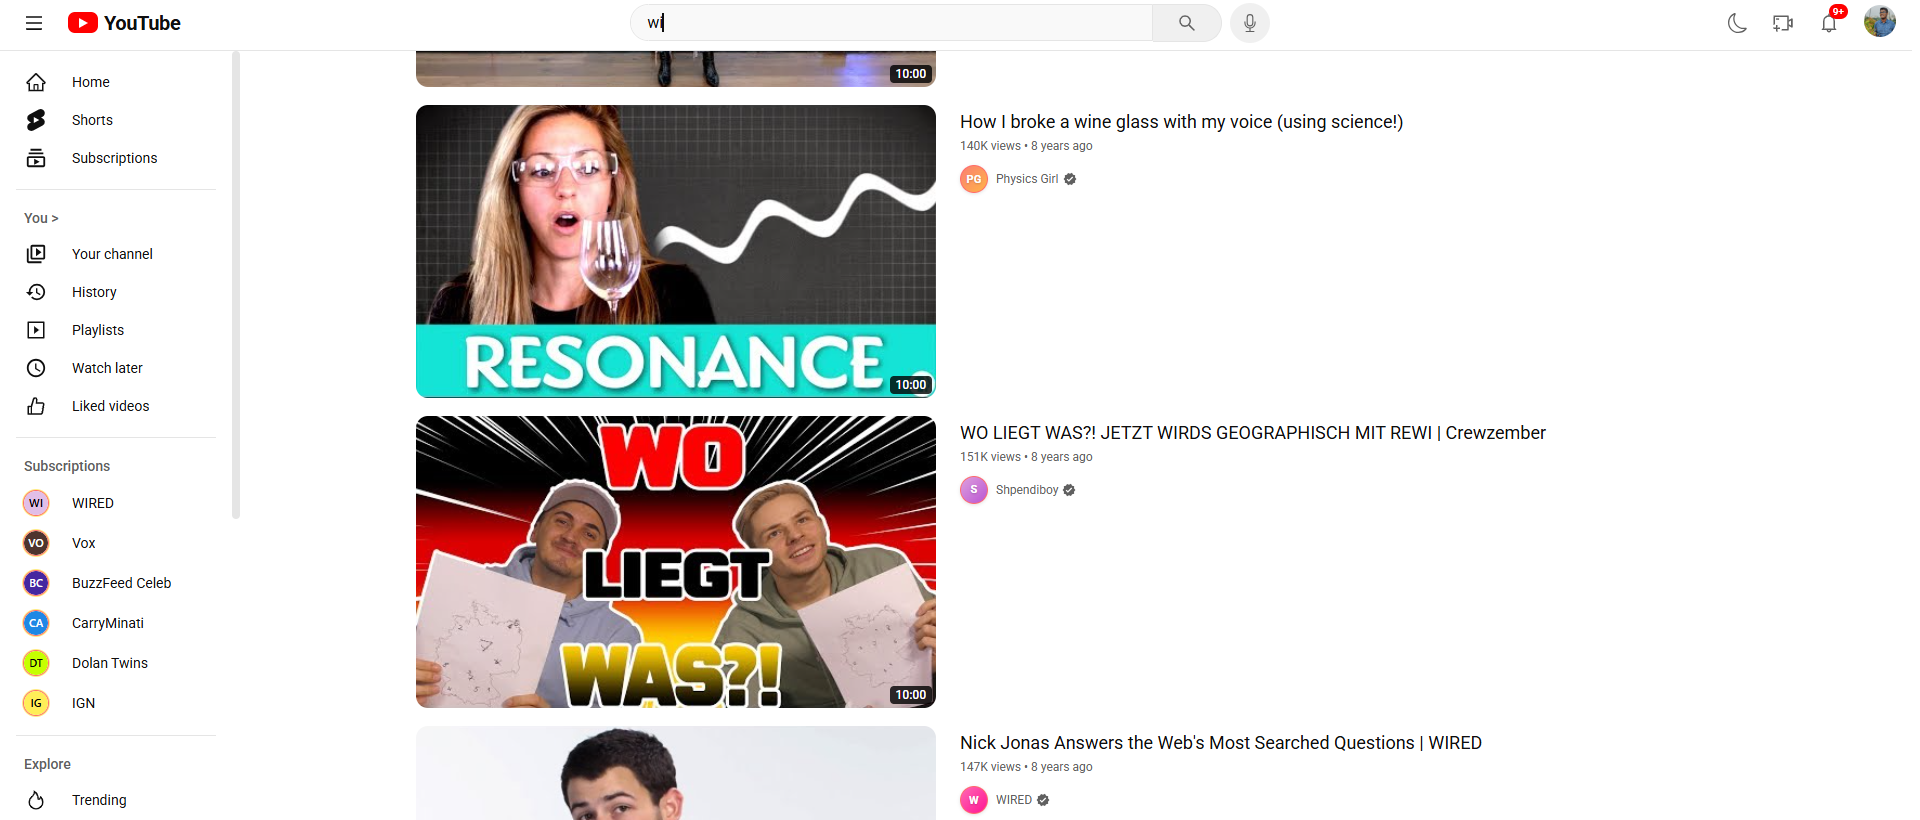
\includegraphics[width=0.9\textwidth]{img-App/Search-keyword-vid.png}
    \vspace{0.3cm}\\
    Keyword-based search results displaying matching videos in a list layout with thumbnails, view counts, channel avatars, and upload dates, ranked using semantic and lexicographic matching.
    \caption{Search Results -- Keyword Video Matches}
    \label{fig:app_search_keyword_vid}
\end{figure}

\begin{figure}[H]
  \centering
    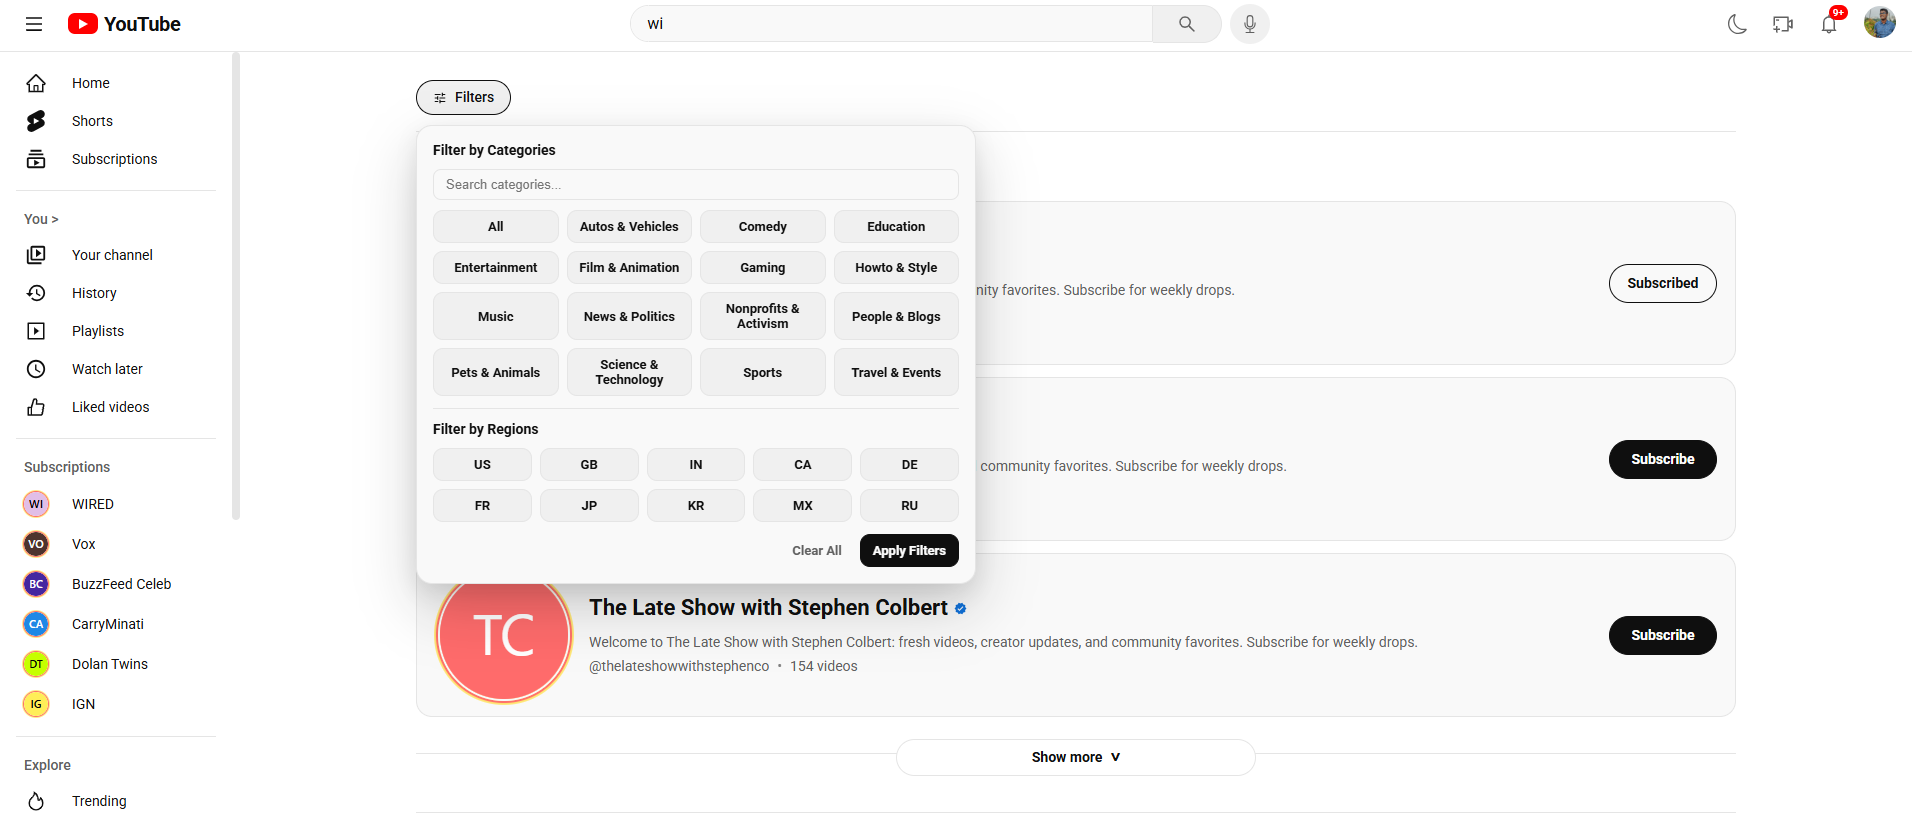
\includegraphics[width=0.9\textwidth]{img-App/Search-Filter.png}
    \vspace{0.3cm}\\
    The search page with the filter dropdown overlay in light mode, allowing users to refine search results by category and region filters.
    \caption{Search Page with Filter Overlay}
    \label{fig:app_search_filter}
\end{figure}

\begin{figure}[H]
  \centering
    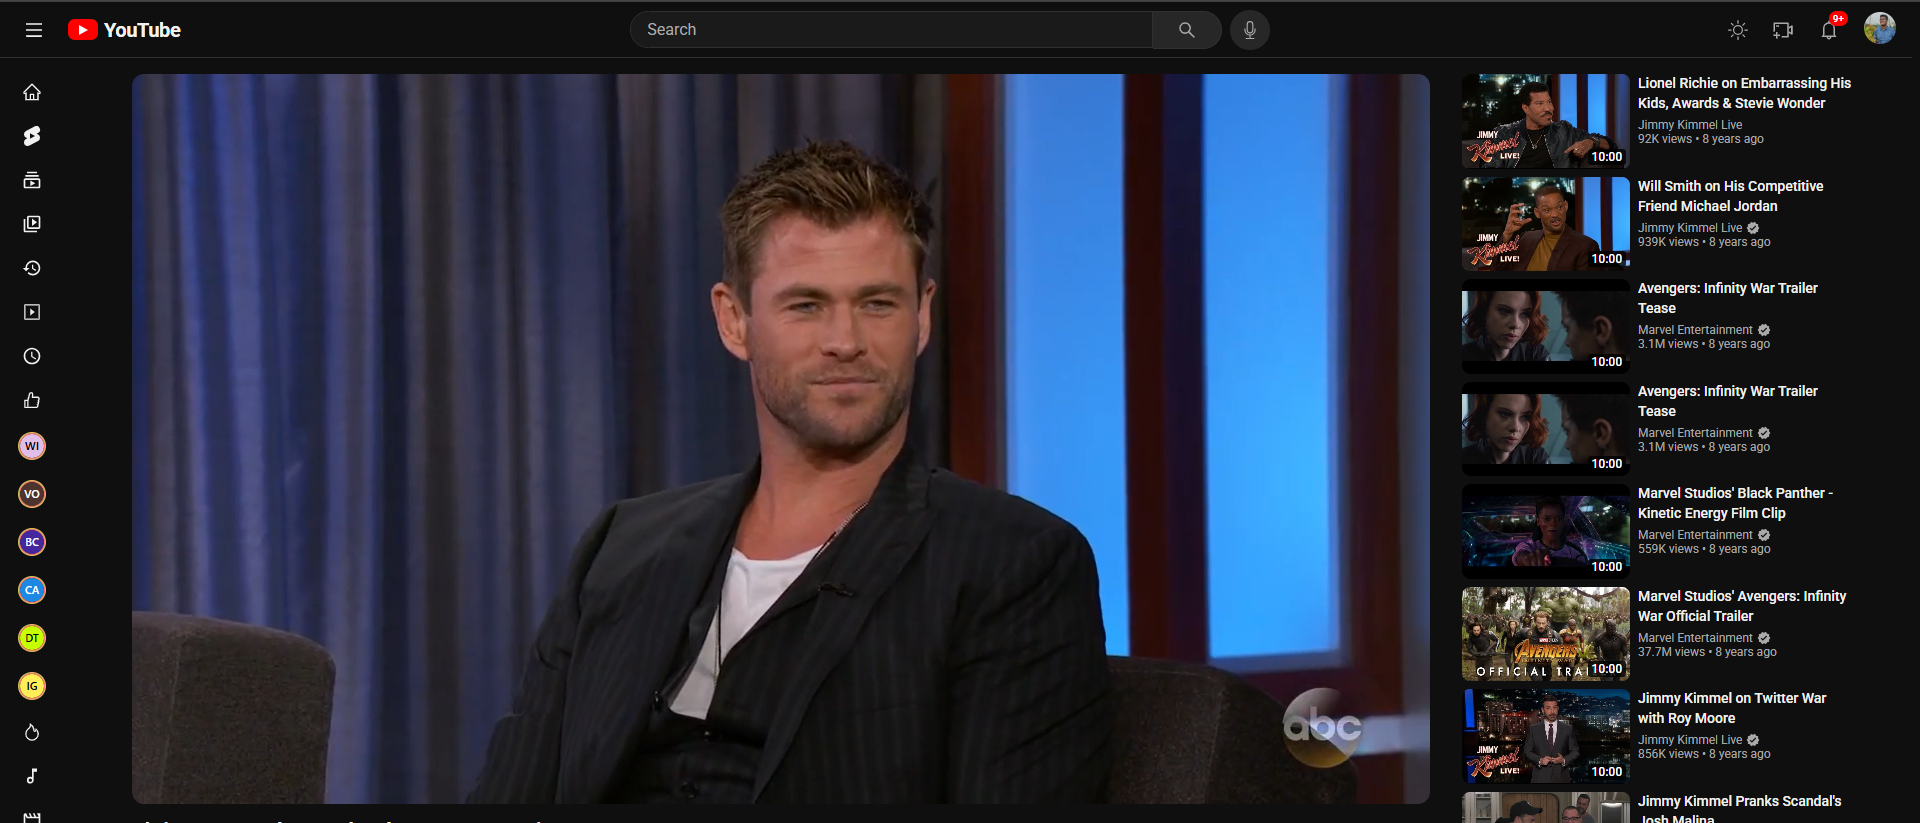
\includegraphics[width=0.9\textwidth]{img-App/VideoPlayer.png}
    \vspace{0.3cm}\\
    The video playback interface in dark mode, showing the primary video player alongside a sidebar of semantically recommended videos for continued viewing.
    \caption{Video Player Interface}
    \label{fig:app_videoplayer}
\end{figure}

\begin{figure}[H]
  \centering
    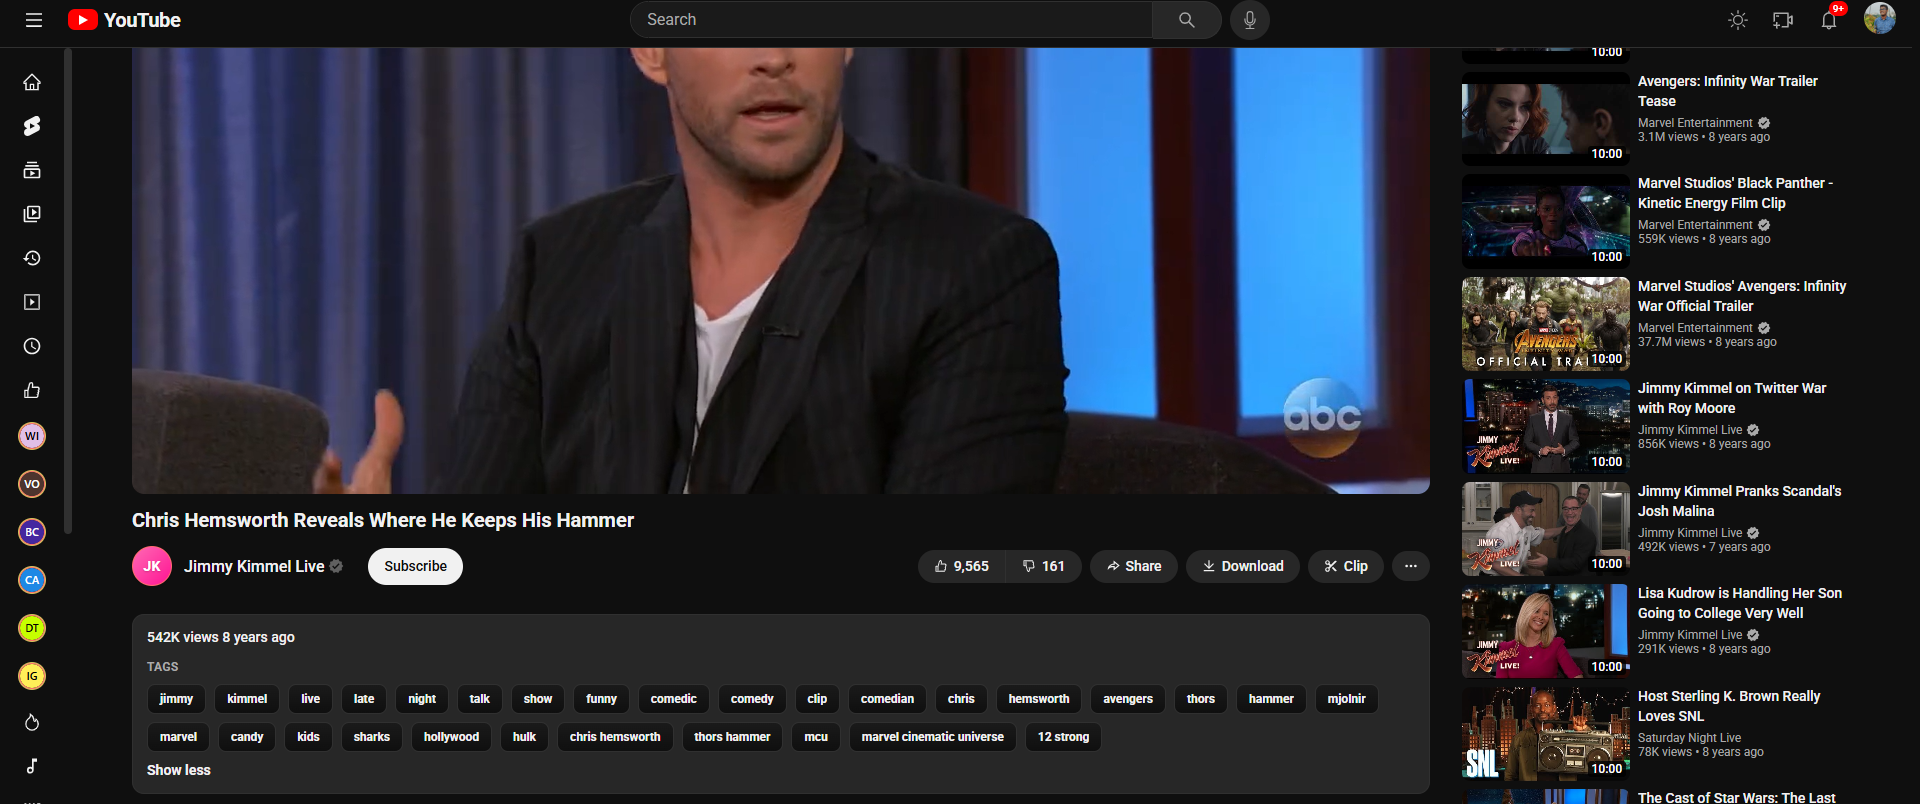
\includegraphics[width=0.9\textwidth]{img-App/VideoPlayer-Desc.png}
    \vspace{0.3cm}\\
    The video player with the description section expanded, displaying the video title, view count, action buttons (like, share, download, clip), channel info with subscribe button, and auto-generated tags.
    \caption{Video Player with Expanded Description}
    \label{fig:app_videoplayer_desc}
\end{figure}

\section{System Architecture Overview}
Our system follows a \textbf{layered monolithic architecture} with a single React client, a single FastAPI backend service, and a managed Supabase data platform.

\subsection{Tech Stack}
\begin{itemize}
    \item \textbf{Frontend:} React 18 + Vite SPA with React Router for navigation, Context API for auth/theme state, and a dedicated service layer for backend communication. Supabase JS SDK handles OAuth and session management on the client side.
    \item \textbf{Backend:} Python FastAPI application exposing REST endpoints for feed generation, watch events, search, recommendations, channel data, and auth/profile operations. Internally modular with separate layers for API routes, core recommendation logic, schemas, and utilities---deployed as a single service.
    \item \textbf{Database \& Search:} PostgreSQL hosted on \textbf{Supabase} with the \texttt{pgvector} extension (HNSW index) for persistent semantic retrieval, supplemented by an in-memory \textbf{FAISS} index bootstrapped at startup for low-latency nearest-neighbor queries.
\end{itemize}

\subsection{Layered Organization}
\begin{enumerate}
    \item \textbf{Presentation Layer} --- React pages/components render UI and trigger API calls.
    \item \textbf{API Layer} --- FastAPI route modules handle validation, auth dependencies, and orchestration.
    \item \textbf{Domain Layer} --- Recommendation strategies, embedding logic, and ranking rules.
    \item \textbf{Data Access Layer} --- Supabase REST/RPC interaction for videos, history, likes, subscriptions, and profiles.
    \item \textbf{Data Layer} --- Supabase PostgreSQL with pgvector for relational + vector storage.
\end{enumerate}

\subsection{Authentication \& User Modes}
The platform supports two interaction modes:
\begin{itemize}
    \item \textbf{Authenticated users:} Supabase OAuth/JWT identity with server-tracked watch history, likes/dislikes, and region preferences.
    \item \textbf{Guest users:} \texttt{localStorage}-driven session and history on the frontend, with dedicated guest endpoints for feed and watch continuity.
\end{itemize}

\subsection{Request Flow}
\begin{enumerate}
    \item User action in React UI (feed load, search, watch, like, etc.).
    \item Frontend service layer calls the corresponding FastAPI endpoint.
    \item FastAPI route invokes recommendation/search/business modules.
    \item Data is fetched from Supabase (REST/RPC) and/or the FAISS in-memory index.
    \item Backend returns the transformed payload to the frontend for rendering.
\end{enumerate}

\section{Implementation Details: Data Curation \& Recommendation Logic}

\subsection{Dataset Aggregation \& Curation}
We curated a dataset of $\sim$24,500 unique videos across 10 regions from YouTube Trending CSVs. Each country's data was processed through a multi-step pipeline:

\begin{enumerate}
    \item \textbf{Deduplication \& Trending Frequency:} Videos appearing multiple times in a country's trending list were deduplicated (keeping the most recent snapshot), and the number of trending appearances was recorded as \texttt{trending\_frequency}.

    \item \textbf{Embed Verification:} A custom browser-based tool (\texttt{verifier.html}) tested every video ID by attempting to instantiate a YouTube IFrame embed with 4 concurrent workers and a 2.5\,s timeout. Videos that fired the \texttt{onReady} event were marked embeddable; those that returned an \texttt{onError} or timed out (geo-blocked, age-gated, or permission-restricted) were discarded.

    \item \textbf{Category Mapping:} Numerical \texttt{category\_id} values were replaced with human-readable category names (e.g., 10 $\rightarrow$ ``Music'') to provide semantic grounding for downstream embeddings.

    \item \textbf{Velocity Score:} To rank virality beyond raw view counts, we engineered a composite score that rewards engagement and positive sentiment:
    $$\text{Velocity} = \text{Trend Freq} \times \log_{10}(\text{Views} + 1) \times \underbrace{\frac{\text{Likes} + \text{Comments}}{\text{Views}}}_{\text{Engagement Rate}} \times \underbrace{\frac{\text{Likes}}{\text{Likes} + \text{Dislikes}}}_{\text{Sentiment Bias}}$$
    The raw score is Min-Max normalized to $[0, 100]$ \textit{per country} to ensure cross-region parity.

    \item \textbf{Mega-String Construction:} For each video, a structured text blob was assembled as:
    \begin{center}
    \texttt{Title: <title> | Category: <name> | Tags: <cleaned tags>}
    \end{center}
    This mega-string serves as the input to the \texttt{BAAI/bge-m3} embedding model, combining title semantics, category context, and tag keywords into a single representation.
\end{enumerate}

\subsection{Embeddings \& Semantic Search}
Numerical category IDs were replaced with semantic Category Names to anchor recommendations. We used the HuggingFace \texttt{BAAI/bge-m3} model to encode titles, tags, and categories into 1024-dimensional vector embeddings offline, enabling multilingual semantic matching beyond keyword overlap. For real-time search queries, an ONNX-quantized (int8) variant of the same model is used on the backend to embed user queries with lower latency.

At startup, the backend loads $\sim$5,000 sampled video embeddings into a \textbf{FAISS IndexFlatIP} index for sub-10\,ms cosine similarity search. Persistent storage remains in Supabase PostgreSQL with \texttt{pgvector} (HNSW index), while FAISS serves as the in-memory serving layer.

\subsection{Taste Vector Construction}
A user's \textbf{Taste Vector} is a weighted average of their watched and liked video embeddings:
\begin{itemize}
    \item \textbf{Time decay:} $w_{\text{decay}} = e^{-\Delta t\,/\,\tau}$, where $\tau = 14$ days.
    \item \textbf{Watch duration boost:} $w_{\text{dur}} = \sqrt{\text{duration} / \text{max\_duration}}$.
    \item \textbf{Like multiplier:} Liked videos receive $2\times$ weight over watches.
    \item The final taste vector is the L2-normalized weighted mean of all contributing embeddings.
\end{itemize}
After the initial build, subsequent watch/like events update the taste vector incrementally via \textbf{Exponential Moving Average} ($\alpha = 0.15$), avoiding any database round-trip.

\subsection{3-Phase Personalization Strategy}
Feed generation follows a three-phase approach that progressively increases semantic personalization as the user accumulates interactions.

\subsubsection{Phase 1: Cold Start (0 interactions)}
For brand-new users with no history, the feed is purely trending-based:
\begin{itemize}
    \item 50\% Global Trending (sorted by velocity score).
    \item 50\% Local Trending (user's region).
\end{itemize}

\subsubsection{Phase 2: Warm-Up (1--4 interactions)}
As the user begins interacting, semantic signals are gradually introduced:
\begin{itemize}
    \item \textbf{1--2 interactions:} 20\% Semantic (FAISS) + 50\% Global Trending + 30\% Local Trending.
    \item \textbf{3--4 interactions:} 40\% Semantic (FAISS) + 35\% Global Trending + 25\% Local Trending.
\end{itemize}

\subsubsection{Phase 3: Fully Personalized (5+ interactions)}
The system transitions to a \textbf{4-Bucket} strategy with adaptive allocation:

\begin{center}
\renewcommand{\arraystretch}{1.2}
\begin{tabular}{l c c c}
    \toprule
    \textbf{Bucket} & \textbf{5--9} & \textbf{10--19} & \textbf{20+} \\
    \midrule
    Semantic / Same Region  & 60\% & 70\% & 75\% \\
    Semantic / Foreign Mix   & 20\% & 15\% & 15\% \\
    Trending / User Region   & 10\% & 10\% & 7\%  \\
    Trending / Global        & 10\% & 5\%  & 3\%  \\
    \bottomrule
\end{tabular}
\end{center}

For the foreign-mix bucket, users with fewer than 10 interactions get randomly sampled foreign regions, while users with 10+ interactions use a \textbf{country-affinity score} (mean cosine similarity of the taste vector against each country's video pool) to weight foreign region selection.

\subsection{Hybrid Search \& Context-Aware Recommendations}
\begin{itemize}
    \item \textbf{Search:} Queries are embedded via \texttt{bge-m3}, then FAISS retrieves candidates which are re-ranked using a hybrid score: 70\% semantic similarity + 20\% keyword match + 10\% category boost.
    \item \textbf{Context-aware recommendations} (``Up Next''): Given the currently playing video's embedding, FAISS retrieves similar videos, re-ranked with shared-keyword and same/related-category affinity bonuses.
\end{itemize}

\section{Deployment Details}
\begin{itemize}
    \item \textbf{Frontend Hosting:} Vercel (\url{https://youtube-clone-frontend-olive.vercel.app})
    \item \textbf{Backend Hosting:} Modal (\url{https://nawrizaturjo03--youtube-clone-backend-web.modal.run})
    \item \textbf{Database:} Supabase (\url{https://supabase.com/dashboard/project/gqpxcspldebemsbpfpfi})
\end{itemize}

\pagebreak

\section{Feature Implementation Contribution Summary}
\begin{table}[h]
    \centering
    \renewcommand{\arraystretch}{1.3}
    \begin{tabularx}{\textwidth}{l X}
        \toprule
        \textbf{Member} & \textbf{Specific Implementation Contributions} \\
        \midrule
        \textbf{Nawriz Ahmed Turjo (2105032)} & Frontend and API Integration, Filtering Implementation, FAISS Optimization and Hosting \\
        \textbf{Abhishek Roy (2105033)} & Dataset curation, Database Hosting and Population, Frontend and UI-UX, Recommendation Engine \\
        \textbf{Monjur Hossain Khan (2105043)} & Base Frontend UI, Authentication, Database Creation, Hosting \\
        \textbf{Shams Hossain Simanto (2105048)} & Backend, API Creation, Recommendation Engine \\
        \textbf{Amit Saha (2105049)} & CI/CD Pipeline, API Unit Test Integration \\
        \textbf{Md. Abrar Jahin (2105055)} & Backend, API Creation, Recommendation Engine, Model Quantization \\
        \bottomrule
    \end{tabularx}
\end{table}

\end{document}